\documentclass[useAMS,usenatbib]{mn2e}

%%%%% AUTHORS - PLACE YOUR OWN MACROS HERE %%%%%
\newcommand{\conj}[1]{\overline{#1}}
\newcounter{NameOfTheNewCounter}
\setcounter{NameOfTheNewCounter}{1}
\newtheorem{theorem}{Theorem}[NameOfTheNewCounter]
\newtheorem{lemma}[theorem]{Lemma}
\newtheorem{proposition}[theorem]{Proposition}
\newtheorem{corollary}[theorem]{Corollary}
\newtheorem{definition}[theorem]{Definition}
\usepackage{graphicx}
%\usepackage[sc]{mathpazo}
\usepackage{amsmath}
\usepackage{multirow}
\usepackage{graphicx}
\usepackage{caption}
\usepackage[T1]{fontenc}
\usepackage[utf8]{inputenc}
\def\lp{\frac 1 {l_{0}}}
\def\kp{\frac 1 {m_{0}}}
\newcommand{\Gcal}{\bmath{\mathcal{G}}}
\newcommand{\Rcal}{\bmath{\mathcal{R}}}
\newcommand{\Mcal}{\bmath{\mathcal{M}}}
\newcommand{\Fcal}{\bmath{\mathcal{F}}}
\newcommand{\GG}{\bmath{G}}

\newcommand{\aaps}{A\&AS}
\newcommand{\aap}{A\&A}
\newcommand{\mnras}{MNRAS}
\newcommand{\nat}{Nature}
\newcommand{\physrep}{Phys. Rep.}

\newcommand{\ee}{\mathrm{e}}
\newcommand{\ii}{\mathrm{i}}

%%%%%%%%%%%%%%%%%%%%%%%%%%%%%%%%%%%%%%%%%%%%%%%%

\title[Correlator Windowing Functions For Cheaper Surveys]{Signals Correlation Algorithms For Cheaper Surveys: Using Windowing Functions. 
}
\author[M. T. Atemkeng , O. M. Smirnov, C. Tasse, G. Foster and J. Jonas]{M. T. Atemkeng$^{1}$, O. M. Smirnov$^{12}$\thanks{E-mail: m.atemkeng@gmail.com}, 
 C. Tasse$^{123}$, G. Foster$^{12}$, J. Jonas$^{12}$ \\
$^1$Department of Physics and Electronics, Rhodes University, PO Box 94, Grahamstown, 6140, South Africa\\
$^2$SKA South Africa, 3rd Floor, The Park, Park Road, Pinelands, 7405, South Africa\\
$^3$GEPI, Observatoire de Paris, CNRS, Universite Paris Diderot, 5 place Jules Janssen, 92190 Meudon, France}
\begin{document}

\date{in original form 2014 Mai 11}

\pagerange{\pageref{firstpage}--\pageref{lastpage}} \pubyear{2013}

\maketitle

\label{firstpage}

\begin{abstract}
This paper investigates the use of baseline dependent windowing functions in interferometry data to minimize the loss of 
signal amplitude (smearing) when the correlated data is averaged over wide bandwidth and long time. In radio interferometry smearing is 
reduced when a cross-correlator averages the correlated data over narrower bandwidth and shorter integration times. Unfortunately, this 
leads to a huge amount of data to manage and it is becoming a bottleneck for further data processing such as calibration and 
imaging.  With future generation surveys, it is important to investigate the reduction of the output data rate. Therefore, the focus of 
this paper is on the use of baselines dependent windowing functions to keep smearing down at an acceptable extent and at the same time 
significantly suppress signals 
from out field of view sources, while the nominal sensitivity is conserved. 
\end{abstract}
\begin{keywords}
Instrumentation: interferometers, Methods: data analysis, Methods: numerical, Techniques: interferometric
\end{keywords}

\section[]{Introduction}

A radio interferometer measures complex quantities called \emph{visibilities}, which, following the van Cittert-Zernike 
relation \citep{tms}, correspond to Fourier modes of the sky brightness distribution, corrupted by various instrumental 
and atmospheric effects. One particular effect, known as \emph{time} and \emph{bandwidth smearing} (or averaging) occurs 
when the visibilities are averaged over a time and frequency bin of non-zero extent. This unavoidably happens in the correlator 
(since the correlator output is, by definition, an average measurement over some interval), but also if data is further 
averaged post-correlation (both for purposes of compression, and to reduce computational cost).

The effect of smearing is mainly a decrease in the amplitude of off-axis sources. This is easy to understand: the visibility contribution of a point source of flux $S$ located in the direction given by the unit vector $\bmath{\sigma}$ is given by

\begin{equation}
V = S \exp \big \{  \frac{2\pi i}{\lambda} \bmath{u}\cdot(\bmath{\sigma}-\bmath{\sigma}_0) \big \},
\end{equation}

where $\bmath{u}$ is the baseline vector, and $\bmath{\sigma}_0$ is the phase centre (or fringe stopping centre) of the observation.
The complex phase term above rotates as a function of frequency (due to the inverse scaling with $\lambda$) and time (due to
the fact that $\bmath{u}$ changes with time, at least in an Earth- or orbit-based interferometer). 
Taking a vector average over a time/frequency bin then results  in a net loss of amplitude. The effect increases 
with baseline length and distance from phase centre. Besides reducing apparent source flux, smearing also distorts the PSF, since different baselines (and thus different Fourier modes) are attenuated differently.

In the era of big interferometers, where computation (and thus data size) becomes one of the main cost drivers, it is 
in principle desirable to average the data down as much as possible, without compromising the science goals. There are natural limits to this: firstly, we still need to critically sample the $uv$-plane, secondly, we need to retain sufficient spectral resolution, thirdly, we don't want to average (at least pre-calibration) beyond the natural variation of the calibration parameters, and fourthly, we want to keep smearing at acceptable levels in order not to lose too much signal. In this work, we concentrate specifically on the smearing problem. Here, we can identify two regimes:

\begin{itemize}
\item In a compact interferometer, the maximum usable field of view (FoV) corresponds to the primary beam (PB) of the antennas; in
most cases (but surveys especially) we want the effective FoV to reach this limit. This imposes an upper limit on the size of a 
time/frequency bin: it must be small enough to keep amplitude loss acceptably low across the entire PB FoV. 
\item In VLBI, smearing is a lot more severe, so the effective FoV is determined by the smallest time/frequency bin size that a
correlator can support, and is normally much smaller than the PB. Modern VLBI correlators overcome this by employing a technique 
called multiple phase centre correlation, where the signal is correlated relative to multiple phase centres simultaneously, thus
effectively ``tiling'' the PB by multiple FoVs. This has a computational cost that scales linearly with the number of phase centres.
\end{itemize}

On the other hand, smearing also has a useful side effect. In interferometry, anything outside the desired FoV is unwanted 
signal. However, the PB pattern of any real-life antenna features sidelobes and backlobes 
that extend across the entire sky, albeit at a relatively faint level. The faintness makes sidelobes useless for imaging any 
but the brightest sources: the scientifically usable FoV is that given by the main lobe. However, the 
sum total signal from all the sources in the PB sidelobes, modulated by their PSF sidelobes, contributes an unwanted global 
background called the \emph{far sidelobe confusion noise} (FSCN). This imposes a fundamental sensitivity limit; in older 
telescopes and surveys this was well below the achievable thermal noise and therefore not a worry, but modern and future 
observatories are capable of reaching this limit \citep{Smirnov-FSCN}. Even in observations well above the FSCN, 
individual extremely bright radio sources such as Cyg A or Cas A can contribute confusing signal from even the most distant 
sidelobe: the LOFAR telescope \citep{LOFAR} has to deal with the so-called ``A-team'' sources on a routine basis. Since 
smearing suppresses distant sources, this somewhat alleviates both the FSCN and A-team problems.

When considering a short sequence of visibilities measured by one baseline, we can think of averaging as a convolution of the 
true visibility by a boxcar function corresponding to the $uv$-extent of the averaging bin, followed by sampling at the 
centre of each bin. Convolution in the visibility plane corresponds to multiplication of the image by a \emph{tapering function} 
that is the Fourier transform (FT) of the convolution kernel; the FT of a boxcar is a Jinc-type taper. If
we consider the entire $uv$-plane, averaging is only a pseudo-convolution, since the different $uv$-bins (and thus
their boxcars) will have different sizes and shapes as determined by baseline length and orientation. Still, we can 
qualitatively view smearing  as some kind of cumulative effect of an ensemble of image-plane tapers corresponding to all the 
different boxcars\footnote{For completeness, we should note that  this ``smearing taper'' is not the only tapering effect 
at work in interferometric imaging. Firstly, antennas have a non-zero 
physical extent: a measured visibility is already convolved by the aperture illumination functions (AIFs) of each pair of 
antennas. The resulting image-plane taper is exactly what the PB is. Secondly, most imaging software employs 
convolutional gridding followed by an FFT, which produces an additional taper that suppresses aliasing of sources from 
outside the imaged region.}. 

What if we were to employ weighted averaging instead of simple averaging (whether in the correlator, or in post-processing)? 
This would correspond to a  pseudo-convolution of the $uv$-plane by some ensemble of \emph{windowing functions} (WFs), 
different from boxcars, which would obviously yield different image-plane tapers, and thus result in different 
smearing response. Filter theory suggests that a WF can be tuned to achieve some desired tapering response. 
An optimal taper would be one that was maximal across the desired FoV, and minimal outside it. In this work, 
we apply filter theory to derive a set of correlator WFs (CWFs) that approximate this more optimal smearing 
behaviour. The trade-off is an increase in thermal noise, since minimum noise can only be achieved with 
unweighted averaging. We show that this effect can be partially mitigated through the use of \emph{extended WFs}. 

{\bf Cite Offringa and LOFAR.}

In the era of the Square Kilometre Array (SKA) and its pathfinders, where dealing with the huge data volumes is one of
the main challenges, use of CWFs potentially offers additional leverage in optimizing radio observations. 
Decreased smearing across the FoV allows for more agressive data averaging, thus reducing storage and compute costs. 
The trade-off is a loss of sensitivity, which pushes up observational time requirements. However, sinc

 N and A-team signal 
could, conceivably, make up for the loss in nominal sensitivity. In the VLBI regime, use of CWFs potentially offers an increase in 
effective FoV at a given correlator dump rate, or equivalently, the ability to tile the PB FoV with fewer phase centres, allowing
for smaller correlators.

\section{Overview and problem statement}

\newcommand{\VV}{\mathcal{V}}
\newcommand{\WW}{\mathcal{W}}
\newcommand{\II}{\mathcal{I}}
\newcommand{\IID}{\mathcal{I}^\mathrm{D}}
\newcommand{\IIDI}{\mathcal{I}^\mathrm{DI}}
\newcommand{\EE}{\mathcal{E}}
\newcommand{\FF}{\mathcal{F}}
\newcommand{\HH}{\mathcal{H}}
\newcommand{\TT}{\mathcal{T}}
\newcommand{\uu}{\bmath{u}}

The following formalism deals with visibilities both as functions (i.e. entire distributions on the $uv$-plane), 
and single visibilities (i.e. values of those functions at a specific point). To avoid confusion between functions in
functional notation and their values, we will use $\VV$ or 
$\VV(u,v)$ to denote functions, and $V$ to denote individual visibilities. Likewise, $\II(l,m)$ denotes a function 
on the $lm$-plane i.e. an image. The symbol $\delta$ always denotes a function, that is a delta-function.

Depending on whether we want to consider polarization or not, $\VV$ can be taken to represent either 
scalar (complex) visibilities, or $2\times2$ complex visibility matrices  as per the radio interferometer 
measurement equation (RIME) formalism \citep{smirnov2011revisiting}. Likewise, $\II$ can be treated as a scalar 
(total intensity) image, or a $2\times2$ brightness matrix distribution. The derivations below 
are valid in either case.

We shall use the symbols $\mathbf{u}=(u,v)$ or $\mathbf{u}=(u,v,w)$ to represent baseline coordinates in units of wavelength, and 
$\mathbf{u}^\mathrm{m}$ for units of metres, with $\mathbf{u} = \mathbf{u}^\mathrm{m}/\lambda = \mathbf{u}^\mathrm{m}\nu/c$

\subsection{Visibility and relation with the sky}
\label{sec:visSky}
An interferometer array measures the quantity $\VV(u,v,w)$, known as the visibility function.
Here, the coordinates $u,v$ and $w$ are vector components in units of wavelength, describing the distance between 
two antennas $p$ and $q$, called the \emph{baseline}. The $w$ axis is oriented towards the \emph{phase centre} of the observation,
while $u$ points East and $v$ North. Given a sky distribution $\II(l,m)$, where $l,m$ are the direction cosines,
the nominal observed visibility is given by the van 
Cittert-Zernike theorem \citep{thompson1999fundamentals} as
\begin{equation}
\VV^\mathrm{nom}(u,v) =\iint\limits_{lm} \frac{\II(l,m)}{\sqrt{1-l^2 - m^2}}\,\ee^{-2\pi\ii\phi (u,v,w)}dldm, \label{eq:visSky:nom}
\end{equation} 
where $\phi(u,v,w)=ul+vm+w(n-1)$, and $n=\sqrt{1-l^2 - m^2}$ (the $n-1$ term comes about when fringe 
stopping is in effect, i.e. when 
the correlator introduces a compensating delay to ensure $\phi=0$ at the centre of the field, otherwise the term is simply $n$). 

Given a pair of antennas $p$ and $q$ forming a baseline $\bmath{u}_{pq}=(u_{pq},v_{pq},w_{pq})$, 
and taking into account the \emph{primary beam} patterns $\EE_p(l,m)$ and $\EE_q(l,m)$ that define the directional sensitivity of 
the antennas, this becomes 
\begin{equation}
\VV_{pq}(u,v)=\iint\limits_{lm} \frac{\EE_p \II \EE_q^H}{\sqrt{1-l^2 - m^2}}\,\ee^{-2\pi\ii\phi (u,v,w)}dldm. \label{eq:visSky}
\end{equation} 
Assuming a small field of view ($n\to 1$) and/or a coplanar array ($w=0$), this becomes a 2D Fourier transform (FT):
\begin{equation}
\VV_{pq}(u,v)=\iint\limits_{lm} \EE_p \II \EE_q^H\,\ee^{-2\pi\ii(ul+vm)}dldm. \label{eq:visSky:2D}
\end{equation} 


The effect of the primary beam can alternatively be expressed in terms of a convolution with its FT, the \emph{aperture 
illumination function} (AIF) $\mathcal{A}_p(u,v)$. In functional form:
\begin{equation}
\VV_{pq} = \mathcal{A}_p \circ \VV^\mathrm{nom}_{pq} \circ \mathcal{A}_q^H.\label{eq:visSky:conv}
\end{equation} 



\subsection{Imaging, averaging and convolution}

\label{sec:AvgCon}
Earth rotation causes the baseline to rotate in time, which we can denote by
$\bmath{u}^\mathrm{m}_{pq}=\bmath{u}^\mathrm{m}_{pq}(t)$. The baseline in units of wavelength 
can be treated as a function of frequency and time:
\begin{equation}
\label{eq:uvtf}
\bmath{u}_{pq}(t,\nu) = \bmath{u}^\mathrm{m}_{pq}(t)\nu/c.
\end{equation} 
This, in turn, allows us to express the visibility in eq.~(\ref{eq:visSky:2D}) as 
a continuous function of $t,\nu$:
\begin{equation}
\VV_{pq}(t,\nu)=\iint\limits_{lm} \EE_p \II \EE_q^H\,\ee^{-2\pi\ii(u_{pq}(t)l+v_{pq}(t)m)}dldm. \label{eq:visSky:2Dtf}
\end{equation} 

Synthesis imaging recovers a so-called ``dirty image'' as the inverse Fourier transform of some measured  
visibility distribution $\VV^\mathrm{(m)}$. This is sampled by a number of baselines $pq$ and time/frequency points 
$t_k,\nu_l$. Designating each such sample by the index $pqkl$, we can express the imaging process as
\begin{equation}
\label{eq:imaging}
\II = \FF^H\{ \WW\cdot \VV^\mathrm{(m)} \}  
\end{equation}
where $\WW$ is the (weighted) sampling function -- a ``bed-of-nails'' function that is non-zero at points where we 
are sampling a visibility, and zero elsewhere. 
Since the Fourier transform is linear, this can be represented by a sum of  ``single-nail'' functions $\WW_{pqkl}$:
\begin{equation}
\WW = \sum_{pqkl} \WW_{pqkl} = \sum_{pqkl} W_{pqkl} \delta_{pqkl},
\end{equation}
where $\delta_{pqkl}$ is a delta-function shifted to the $uv$-point being sampled:
\begin{equation}
\delta_{pqkl}(\bmath{u}) = \delta(\bmath{u}-\bmath{u}_{pq}(t_k,\nu_l))
\end{equation}
and $W_{pqkl}$ is the 
associated weight. The Fourier transform being linear, we can rewrite eq.~(\ref{eq:imaging}) as 
\begin{equation}
\label{eq:imaging2}
\II = \sum_{pqkl} W_{pqkl} \mathcal{F}^{-1}[ \VV^\mathrm{(m)}_{pqkl} ],
\end{equation}
where 
\begin{equation}
\label{eq:imaging2a}
\VV^\mathrm{(m)}_{pqkl} = \delta_{pqkl} V^\mathrm{(m)}_{pqkl}
\end{equation}
i.e. is a visibility distribution corresponding to the single visibility sample $pqkl$. We can rewrite eq.~(\ref{eq:imaging})
again as
\begin{equation}
\label{eq:imaging3}
\IID =  \sum_{pqkl} W_{pqkl} \IID_{pqkl},~~
\IID_{pqkl} =  \FF^H\{ \VV^\mathrm{(m)}_{pqkl} \},
\end{equation}
which shows that the dirty image $\IID$ is a weighted sum of dirty images corresponding to the individual visibility 
samples $pqkl$ (each of which is essentially a single fringe pattern).

Were we to measure instantaneous visibility samples, we would have the simple relation of
\begin{equation}
V^\mathrm{(m)}_{pqkl}  = \VV_{pq}(t_k,\nu_l),
\end{equation}
where the right-hand side is given by eq.~(\ref{eq:visSky:2Dtf}). This results in what we'll call the \emph{ideal} dirty image 
$\II^{DI}$:
\begin{equation}
\label{eq:imaging:DI}
\IIDI =  \sum_{pqkl} W_{pqkl} \IIDI_{pqkl},~~
\IIDI_{pqkl} =  \FF^H\{ \delta_{pqkl}\VV_{pq} \},
\end{equation}
However, an interferometer necessarily measures the
average visibility over a rectangular time-frequency bin 
\begin{equation}
\mathsf{B}_{kl} = \bigg [ t_k-\frac{\Delta t}{2},t_k+\frac{\Delta t}{2} \bigg ]
\times
\bigg [ \nu_l-\frac{\Delta\nu}{2},\nu_l+\frac{\Delta\nu}{2} \bigg ],  
\end{equation}
which, ideally, can be represented by an integration:
\begin{equation}
V^\mathrm{(m)}_{pqkl} = \frac{1}{\Delta t \Delta \nu} 
\iint\limits_{\mathsf{B}_{kl}}
\VV_{pq}(t,\nu)d\nu dt.
\label{eq2:conti}
\end{equation}

Inverting the relation of eq.~(\ref{eq:uvtf}), we can change variables to express this as an integration over the 
corresponding bin $\mathsf{B}^{\prime}_{kl}$ in $uv$-space:
\begin{equation}
V^\mathrm{(m)}_{pqkl} = \frac{1}{\Delta t \Delta \nu} 
\iint\limits_{\mathsf{B}^{\prime}_{kl}}
\VV_{pq}(u,v)\bigg| \frac{\partial(t,\nu)}{\partial(u,v)}\bigg| dudv,
\label{eq2:conti:uv}
\end{equation}
where $\mathsf{B}^{\prime}_{kl}$ is the corresponding bin in $uv$-space. While $\mathsf{B}_{kl}$ is rectangular in $t\nu$ space, 
$\mathsf{B}^{\prime}_{kl}$ is an arc segment in $uv$-space. Assuming a bin small enough that 
$\partial\bmath{u}/\partial t$ is approximately constant over the bin, we then have
\begin{equation}
V^\mathrm{(m)}_{pqkl} \sim \iint\limits_{\mathsf{B}^{\prime}_{kl}}
\VV_{pq}(\bmath{u}) d\bmath{u},
\label{eq2:conti:uv1}
\end{equation}

% In actual fact, a correlator (or an averaging operation in post-processing) deals with averages of discrete samples rather than a 
% continuous integration. This can be represented by subdividing the bin $\mathsf{B}_{kl}$ into $n_t\times n_\nu$ samples $\{t_i\}$ and $\{\nu_j\}$, 
% and taking the average. This ignores the complexities of correlator architecture (where the visibilities are channelized 
% via a Fourier transform of a time series, before or after correlation), but it does represent an accurate model 
% of the measured visibility:
% \begin{equation}
% V_{pqkl}^\mathrm{(m)} = \frac{1}{n_t n_{\nu}}  \sum_{i=1}^{n_t}\sum_{j=1}^{n_{\nu}}\VV_{pq}(t_i,\nu_j).\label{eq2:sample}
% %&=&\frac{1}{n_t n_{\nu}}  \sum_{i=1}^{n_t}\sum_{j=1}^{n_{\nu}}\mathcal{\textbf{V}}_{pq,(t,\nu)}^{meas} 
% \end{equation}  

% Let us represent the sampling process via multiplication of $V_{pq}(t,\nu)$ by a ``bed of nails'' sampling function $S_{pq}(t,\nu)$
% that selects points where we sample the discrete visibilities: $V^\mathrm{samp}_{pq} = S_{pq}\cdot V_{pq}$. From this point 
% on we will work with the sampled visibilities $V^\mathrm{samp}$ only. We can now represent the averaging process by a discrete sum:
% Here, $V_{pq,(t,\nu)}$ is a continuous function, in reality we know only the sampled visibility,  
% $V_{pq,(t,\nu)}^{samp}=S_{pq,(t,\nu)}\cdot V_{pq,(t,\nu)}$ at a specific time and frequency. The sampling function, 
% $S_{pq,(t,\nu)}$ indicates where the $(u, v)$ data for the baseline (p,q) are measured  during the 
% integration. It is unity where measurement have been made, and zero otherwise.
% Eq.\ref{eq2:conti} holds for many sources, when the signal at the centre time 
% interval $t_c$ and centre frequency interval $\nu_c$  is 
% restricted to a short time and narrow 
% frequency intervals, this is the current efficient observing mode. However, the mathematics behind is as 
% follows: 
% \begin{equation}
% V_{pq}^\mathrm{(m)}(t_c,\nu_c) = \frac{1}{n_t n_{\nu}}  \sum_{i=1}^{n_t}\sum_{j=1}^{n_{\nu}}V_{pq}(t_i,\nu_j).\label{eq2:sample}
% %&=&\frac{1}{n_t n_{\nu}}  \sum_{i=1}^{n_t}\sum_{j=1}^{n_{\nu}}\mathcal{\textbf{V}}_{pq,(t,\nu)}^{meas} 
% \end{equation}
% Note that we ignores the complexities of correlator architecture (where the visibilities are channelized via 
% a Fourier transform of a time series, before or after correlation), but does represent an accurate model of what is actually 
% measured.
% Here, $V_{pq,(t,\nu)}$ is a continuous function, in reality we know only the sampled visibility,  
% $V_{pq,(t,\nu)}^{samp}=S_{pq,(t,\nu)}\cdot V_{pq,(t,\nu)}$ at a specific time and frequency. The sampling function, 
% $S_{pq,(t,\nu)}$ indicates where the $(u, v)$ data for the baseline (p,q) are measured  during the 
% integration. It is unity where measurement have been made, and zero otherwise.
% Eq.\ref{eq2:conti} holds for many sources, when the signal at the centre time interval $t_c$ and centre frequency interval $\nu_c$  is 
% restricted to a short time and narrow 
% frequency intervals, this is the current efficient observing mode. However, the mathematics behind is as 
% follows: 

% We can represent the underlying ``high-resolution'' sampling process via a multiplication of the continuous
% visibility distribution $\VV_{pq}(t,\nu)$ by a sampling function $\HH_{pq}(t,\nu)$,  which is another ``bed of nails''  
% function that selects the $t,\nu$ points corresponding to the sample points $\{t_i\}$ and $\{\nu_j\}$: 
% \begin{equation}
% \VV^\mathrm{(s)}_{pq} = \HH_{pq}\cdot \VV_{pq}. 
% \end{equation}
% % From this point on  we will work with the sampled visibilities $V^\mathrm{samp}$ only.

Now, let us introduce a \emph{normalized boxcar windowing function}, $\Pi_{pqkl}(t,\nu)$ 
\begin{equation}
\Pi_{pqkl}(t,\nu) = \bigg \{ \begin{array}{cl}
\frac{1}{\Delta t\Delta\nu}, &  |t|\leq\Delta t/2,~~|\nu|\leq\Delta\nu/2 \\
0, & \mathrm{otherwise},
\end{array}
\end{equation}
using which we may re-write eq.~(\ref{eq2:conti}) as
\begin{equation}
V^\mathrm{(m)}_{pqkl} =  
\iint\limits_{\infty}
\VV_{pq}(t,\nu) \Pi_{pqkl}(t-t_k,\nu-\nu_l) dtd\nu,
\end{equation}
which can also be expressed as a convolution:
\begin{equation}
V^\mathrm{(m)}_{pqkl} = [ \VV_{pq} \circ \Pi_{pqkl} ](t_k,\nu_l),
\end{equation}

Likewise, eq.~(\ref{eq2:conti:uv}) can also be rewritten as a convolution in $uv$-space:
\begin{equation}
V^\mathrm{(m)}_{pqkl} = [ \VV_{pq} \circ \Pi^\prime_{pqkl} ](\bmath{u}_{pq}(t_k,\nu_l)),
\label{eq:avscon}
\end{equation}
where $\Pi^\prime_{pqkl}$ is a boxcar-like WF that corresponds to bin $\mathsf{B}^\prime_{kl}$ in $uv$-space 
(and also includes the determinant term of eq.~\ref{eq2:conti:uv}). This makes it explicit that each averaged 
visibility is drawn from a convolution of the underlying visibilities with a boxcar-like WF.

Note what eq. (\ref{eq:avscon}) does and does not say. It does say that each individual averaged visibility corresponds to 
convolving the true visibilities by some WF. However, this WF is different for each baseline $pq$ and 
time/frequency sample $t_k,\nu_l$ (which is emphasized by the subscripts to $\Pi$ in the equations above). Averaging is thus 
not a ``true'' convolution, since the convolution kernel changes at every point in the $uv$-plane. We'll call this 
process a \emph{pseudo-convolution}, and the kernel being convolved with ($\Pi^\prime_{pqkl}$) an example of a 
\emph{baseline-dependent windowing function} (BDWF). In subsequent sections we will explore alternative BDWFs.

In actual fact, a correlator (or an averaging operation in post-processing) deals with averages of discrete 
samples, rather than a continuous integration. To represent this properly, we need to replace the integrals of 
eqs.~(\ref{eq2:conti}-\ref{eq2:conti:uv1}) by the discrete sums:
\begin{equation}
\label{eq:discrete:tf}
V^\mathrm{(m)}_{pqkl} = \sum_{i,j=-\infty}^{\infty}  \VV_{pq}(t_i,\nu_j) \Pi_{pqkl}(t_i-t_k,\nu_j-\nu_l)
\end{equation}
and
\begin{equation}
\label{eq:discrete:uv}
V^\mathrm{(m)}_{pqkl} = \sum_{i,j=-\infty}^{\infty}  \VV_{pq}(\bmath{u}_{ij}) \Pi^\prime_{pqkl}(\bmath{u}_{ij}-\bmath{u}_{kl}),
\end{equation}
of which the first is a conventional discrete convolution (assuming a regular $t\nu$ grid), and the second is a convolution 
on an irregular grid -- the $\bmath{u}_{ij}$ grid being schematically illustrated by Fig.~\ref{fig:uvcov}.

\begin{figure}
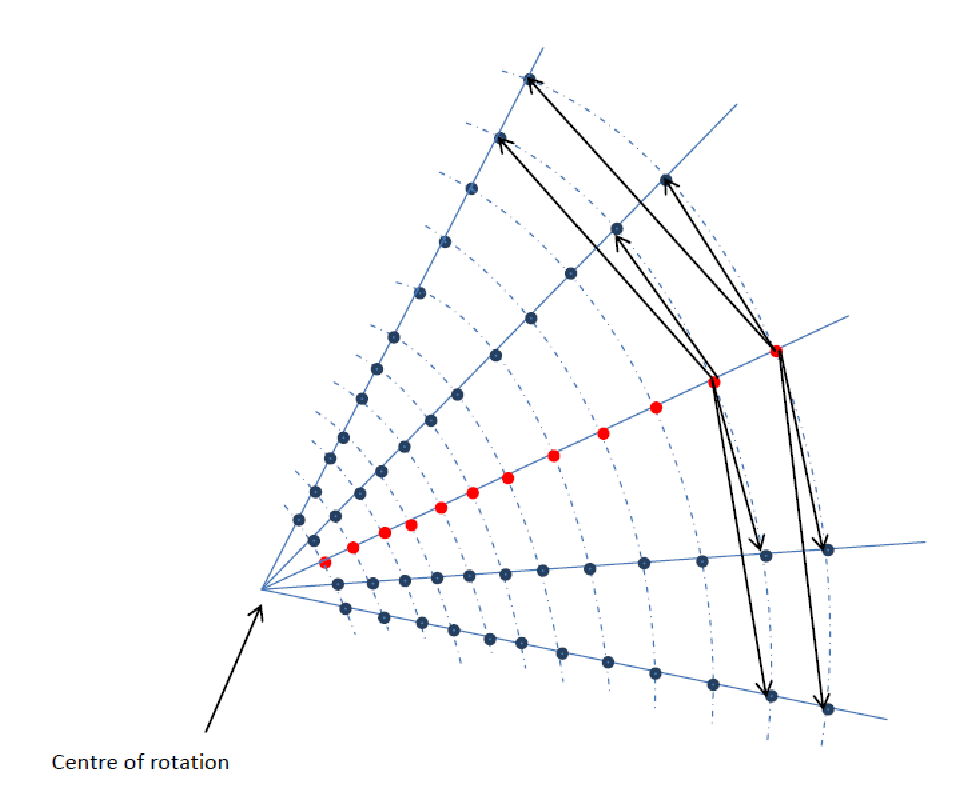
\includegraphics[width=1\columnwidth]{./Figures/uvcov.png}\caption{Schematic of $uv$-coverage for 
regularly spaced time-frequency samples.}\label{fig:uvcov}
\end{figure}


\subsection{Effect of averaging on the image}
\label{sec:effectbw}

\begin{figure*}
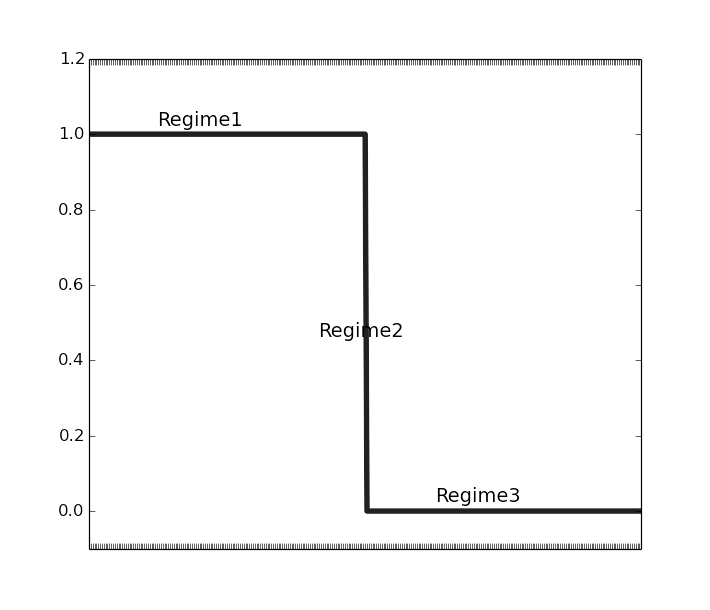
\includegraphics[width=.5\textwidth]{./Figures/idealIPRgrey.png}%
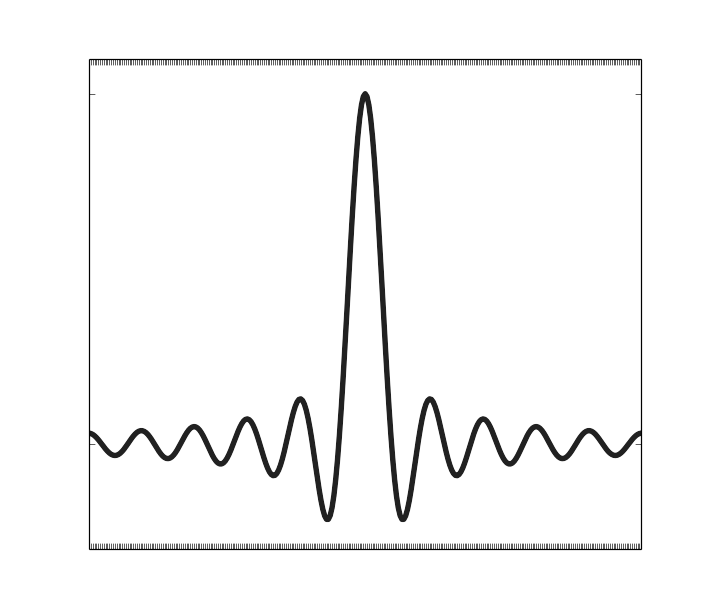
\includegraphics[width=.5\textwidth]{./Figures/idealsincgrey.png}\\
\caption{Left: boxcar response. In the $uv$-plane, this represents the windowing function corresponding to normal
averaging of visibilities. In the image plane, this represents the ideal image-plane tapering function. Right: 
Sinc response. In the image plane, this represents the tapering function corresponding to a boxcar WF in 
the $uv$-plane. In the $uv$-plane, this represents the ideal WF.}
\label{fig:idealWF}
\end{figure*}

In the limit of $\Delta t,\Delta \nu \rightarrow 0$, averaging becomes equivalent to sampling. 
An interferometer must, intrinsically, employ a finitely small averaging interval. The Fourier phase 
component $2\pi\phi(u,v,w)$ is a function of frequency and time, with increasing variation over the averaging interval 
for sources far from the phase centre. The average of a complex quantity with a varying phase then effectively ``washes out'' 
amplitude, the effect being especially severe for wide FoVs \citep[for an extensive discussion, see][]{bregman2012system}. This
effect is often referred to as \emph{time} and \emph{bandwidth smearing}.

The discussion above provides an alternative way to look at smearing. Combining eqs.~(\ref{eq:imaging}--\ref{eq:imaging:DI}) with 
(\ref{eq:avscon}), and using the Fourier convolution theorem, we can see that the dirty image is formed up as
\begin{equation}
\IID =  \sum_{pqkl} W_{pqkl}  \TT_{pqkl} \IIDI_{pqkl},
\end{equation}
where the baseline-dependent \emph{tapering function} $\TT_{pqkl}$ is the inverse FT of the BDWF:
\begin{equation}
\TT_{pqkl} = \FF^H\{ \Pi^{\prime}_{pqkl} \}.
\end{equation}
In other words, the dirty image made from averaged visibilities is a weighted average of the per-visibility ideal dirty images, 
each one multiplies by its own taper. The FT of a boxcar-like function is a sinc-like function, schematically illustrated in one
dimension by Fig.~\ref{fig:idealWF}. Time and bandwidth smearing represents the average effect 
of all these individual tapers. Shorter baselines correspond to smaller boxcars and wider tapers, longer baselines to larger 
boxcars and narrower tapers, and are thus more prone to smearing.

\begin{figure*}
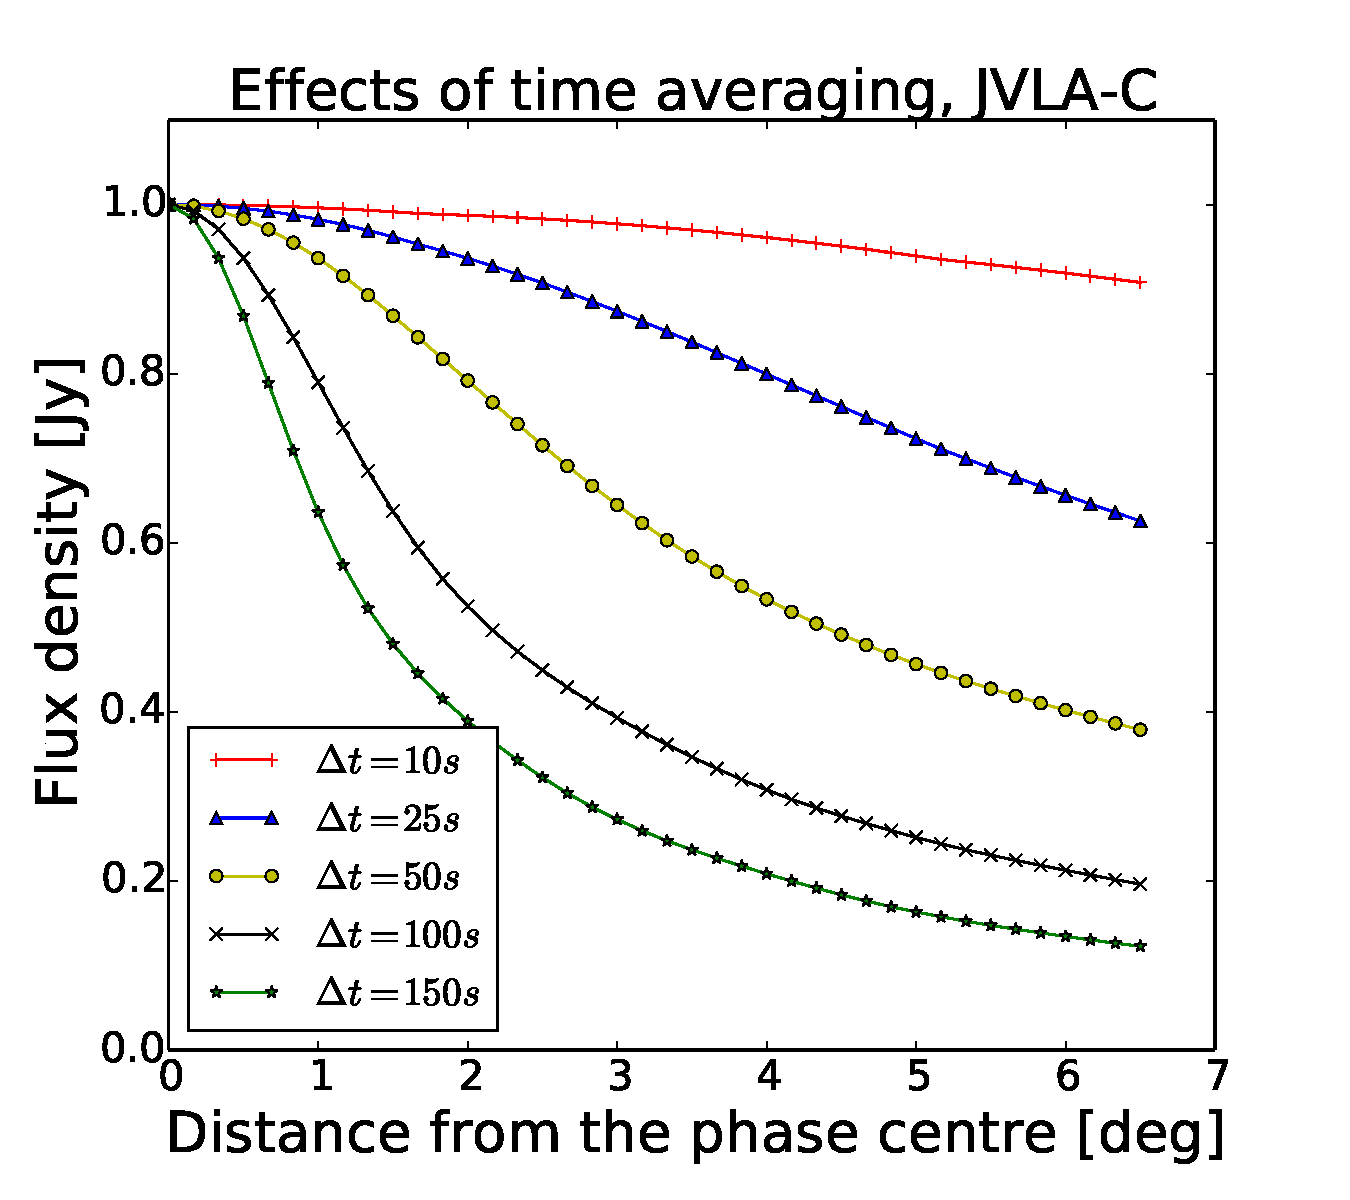
\includegraphics[width=\columnwidth]{./Figures/effect_time_averaging.pdf}%
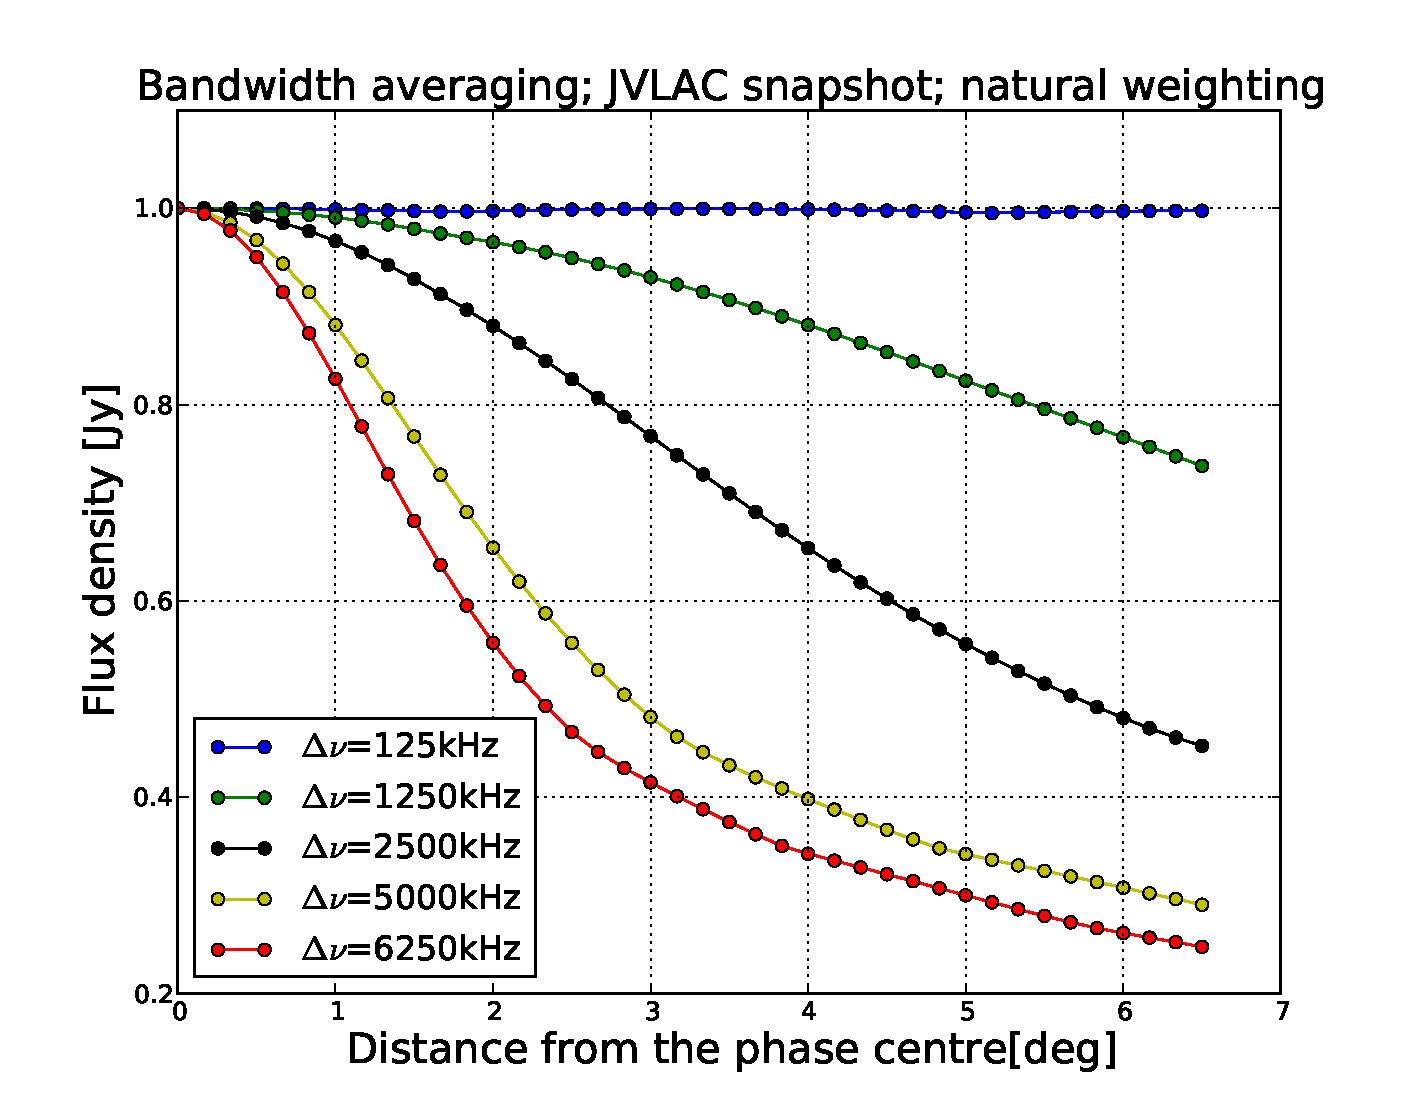
\includegraphics[width=\columnwidth]{./Figures/effect_bandwid_averaging.pdf}
\caption{Effects of time and frequency averaging: the apparent intensity of a 1 Jy source, as seen by JVLA-C at 1.4 GHz, 
as a function of distance from phase centre. (Left) Frequency interval fixed at 125 kHz, time interval varies; 
(right) time interval fixed at 1s, frequency interval varies.}\label{fig:smear}
\end{figure*}

Figure \ref{fig:smear} (produced by simulating a series of high time-frequency resolution observation using MeqTrees, and 
applying averaging) shows the attenuation of a 1 Jy source as a function of distance
from phase centre, for a set of different time and frequency intervals. The simulations correspond to JVLA 
in the C configuration, with an observing frequency of 1.4 GHz. At this frequency, the first null of the PB is at 
$r\approx36'$, and the half-power point is at $\sim16'$, thus we can consider the ``conventional'' FoV (i.e. the half-power 
beam width, or HPBW) to be about $0.5^\circ$ across. Note that the sensitivity of the upgraded JVLA, as well as
improvements in calibration techniques \cite{Perley2013}, allow imaging to be done in the first PB sidelobe as well
(and in fact it may be necessary for deep pointings, if only to deconvolve and subtract sidelobe sources), so we could also
consider an ``extended'' FoV extending out to the second null of the PB at $r\approx1.25^\circ$. Whatever definition
of the FoV we adopt, Fig.~\ref{fig:smear} shows that to keep amplitude losses across
the FoV to within some acceptable threshold, say 1\%, the averaging interval cannot exceed some critical size,
say 10s and 1 MHz. Conversely, if we were to adopt an aggressive averaging strategy for the purposes of data 
compression, say 50s and 5 MHz, the curves indicate that we would suffer substantial amplitude loss towards the 
edge of the FoV. 

Finally, note that the curves corresponding to acceptably low values of smearing across the FoV (i.e. up to 25s and 
up to 1.25 MHz) have a very gentle slope, with very little suppression of sources \emph{outside} the FoV. 

\subsection{The case for alternative BDWFs}

The tapering response induced by normal averaging (Fig.~\ref{fig:smear}) is far from ideal: it either suppresses too much within 
the FoV, or too little outside the FoV, or both. The optimal tapering response would be boxcar-like, as in 
Fig.~\ref{fig:idealWF}(left). The BDWF that would produce such a response is sinc-like, as in Fig.~\ref{fig:idealWF}(right). 
The problem with a sinc is that it has infinite support; applying it over finite-sized bins necessarily means a \emph{truncated} 
BDWF that results in a suboptimal taper. The problem of optimal filtering has been well studied in signal processing (usually
assuming a true convolution rather than the pseudo-convolution we deal with here), and we shall apply these lessons below.

The derivations above make it clear that by using a different BDWF in place of the conventional boxcar-like $\Pi^\prime$ 
could in principle yield more optimal tapering response. The obvious catch is a loss in 
sensitivity. Each visibility sample is subject to an independent Gaussian noise term in the real and imaginary part; the noise of
the average of a set of samples is minimized when the average is naturally weighted (or unweighted, if the noise is 
constant across visibilities). Thus, any deviation from a boxcar WF must necessarily increase the noise in the 
visibilities. Below we will study this effect both theoretically and via simulations, to establish whether this 
trade-off is sensible, and under which conditions.

\section{Overview of windowing functions}
\label{subsec:Windowing functions}

In signal processing, a WF is a mathematical function with limited support (i.e. zero outside some interval). Conventionally,
a time series is convolved with a WF to produce some desired response in the frequency domain. Applying this to our problem
can lead to quite some confusion in terminology. Table~\ref{tab:terms} provides a mapping between the terms commonly used in SP, 
and their conceptual equivalent in BDWFs.

\begin{table}
\begin{tabular}{l|l}
\hline
 \bf Signal processing & \bf BDWFs\\
\hline\hline
Frequency (freq) domain & Image plane \\
Time domain & Fourier plane or $uv$ plane \\
Spectral response\\
~~or freq response & Image plane response (IPR)\\
Time response & Fourier plane response\\
Cut-off time interval  \\
~~or time pass band & $uv$ averaging bin\\
Cut-off freq interval \\
~~or freq pass band, or main lobe & FoV\\
Time stop band & Outside of the $uv$-bin\\
Freq stop band & Outside of the FoV\\
Octave & Doubling in size\\
Normalized freq & Distance from phase centre \\
Band-limited \\
~~(applied to visibilities) & restricted FoV \\
\end{tabular}
\caption{Mapping of terminology between signal processing and BDWFs.}
\label{tab:terms}
\end{table}


WF -- or rather their corresponding image-plane response (IPR) -- can be characterized in terms of various metrics. Some common 
ones are the peak sidelobe level (PSL), the main lobe width (MLW) and the sidelobes roll-off (SLR) rate. In terms of the ``ideal'' 
IPR (Fig.~\ref{fig:idealWF}, left), these correspond to the following desirable traits:

\begin{itemize}
\item Maximally conserve the signal within the FoV (``regime 1'' in the figure), and make the transition in ``regime 2'' as sharp as possible. Both of these correspond to larger MLW.
\item Attenuate sources outside the FoV (``regime 3''): this corresponds to a lower PSL and higher SLR.
\end{itemize}

Below we provide an overview some common (one-dimensional) WFs employed in signal processing.

\subsection{Boxcar window}
\begin{figure*}
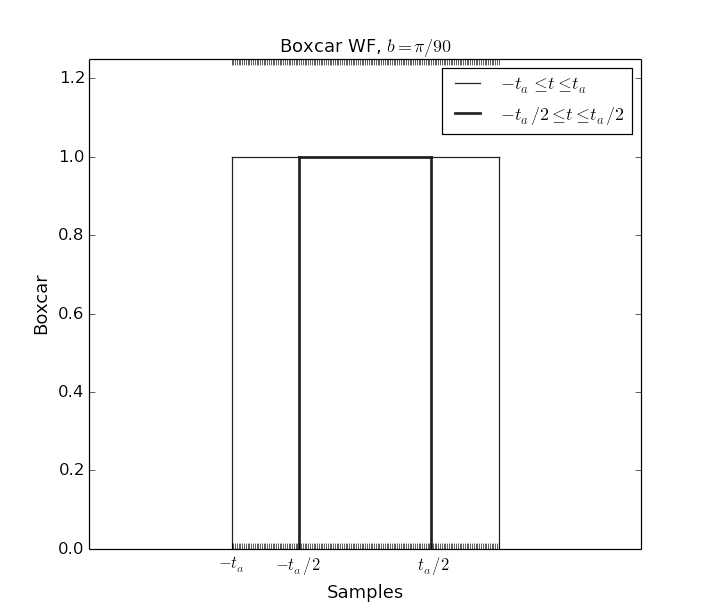
\includegraphics[width=.5\textwidth]{./Figures/boxcargrey.png}%
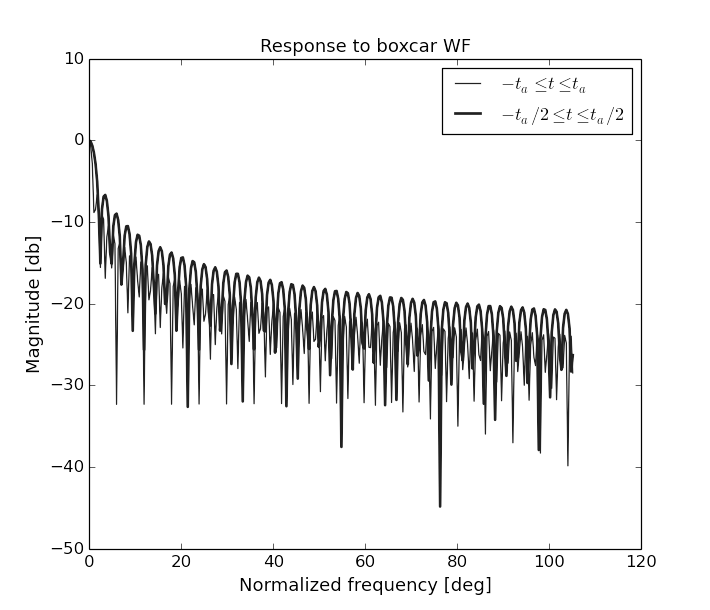
\includegraphics[width=.5\textwidth]{./Figures/freq_resp_boxgrey.png}
\caption{Boxcar windowing function and its tapering response.}\label{fig:wf:box}
\end{figure*}
The boxcar window for a cut-off time interval of $[-t_a,t_a]$ is defined as:
\begin{equation}
\Pi(t)=\left\{
\begin{array}{rl}
1 & \mbox{$-t_a \leq t \leq t_a$} \\
0 & \mbox{otherwise}
\end{array}\right.
\end{equation}
Fig. \ref{fig:wf:box} shows a plot of $\Pi(t)$ and its response. The blue and red curves 
correspond to cut-off time intervals of $[-t_a, t_a]$ and 
$[-t_a/2,t_a/2]$ respectively. Note that when the cut-off time interval is larger, the MLW is 
narrower, and the sidelobes are lower.

The other WFs given below are all multiplied with a boxcar to ensure a cut-off interval of $[-t_a,t_a]$.

\subsection{Gaussian window}
\begin{figure*}
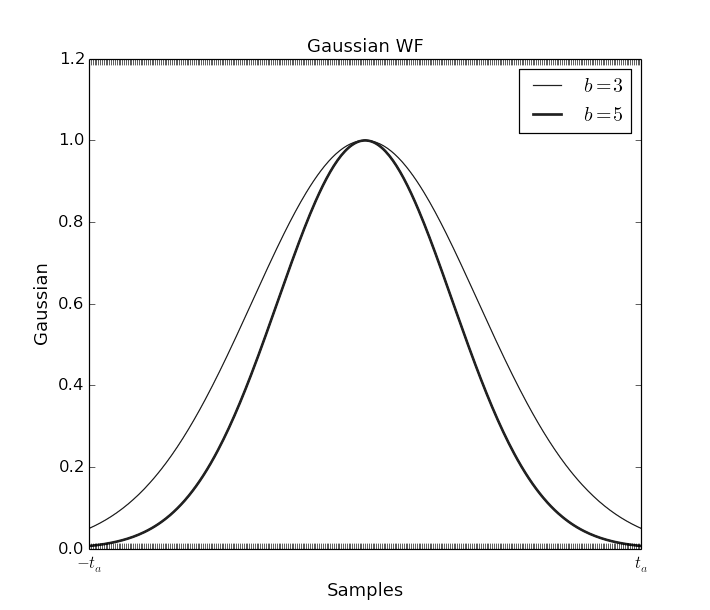
\includegraphics[width=.5\textwidth]{./Figures/gaussiangrey.png}%
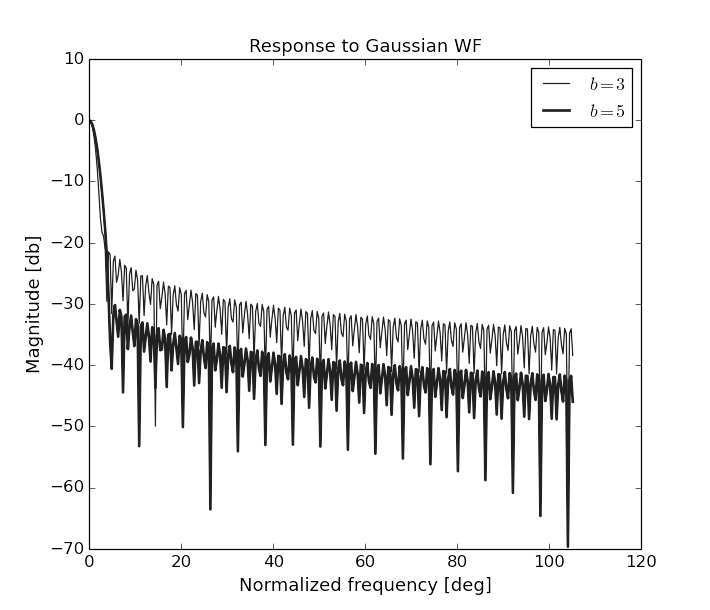
\includegraphics[width=.5\textwidth]{./Figures/freq_resp_gaussiangrey.png}
\caption{Gaussian windowing function and its tapering response.}\label{fig:wf:gauss}
\end{figure*}
A Gaussian WF centred at zero with a standard deviation of $\sigma_1$ is given by: 
\begin{equation}
  G(t)= \Pi(t) e^{-bt^{2}}, \label{eq:gauss}
\end{equation}
where $b=(2\sigma_1^2)^{-1}$. The FT of the Gaussian term is given by 
$\mathcal{F}\big\{G(t)\big\}=\sqrt{\frac{b}{\pi}}e^{-cl^2}$, where $c=\pi^2/b$, i.e.
is also a Gaussian with standard deviation of $\sigma_2= (2\pi\sigma_1)^{-1}$.

Fig. \ref{fig:wf:gauss} shows a plot of $G(t)$ and its response. The WF is truncated at $[-t_a,t_a]$, with $b = 3$ for the blue curve and $b=5$ for the red curve. Its response is characterized by extremely low sidelobes, but a narrow main lobe.

\subsection{Butterworth window}
\begin{figure*}
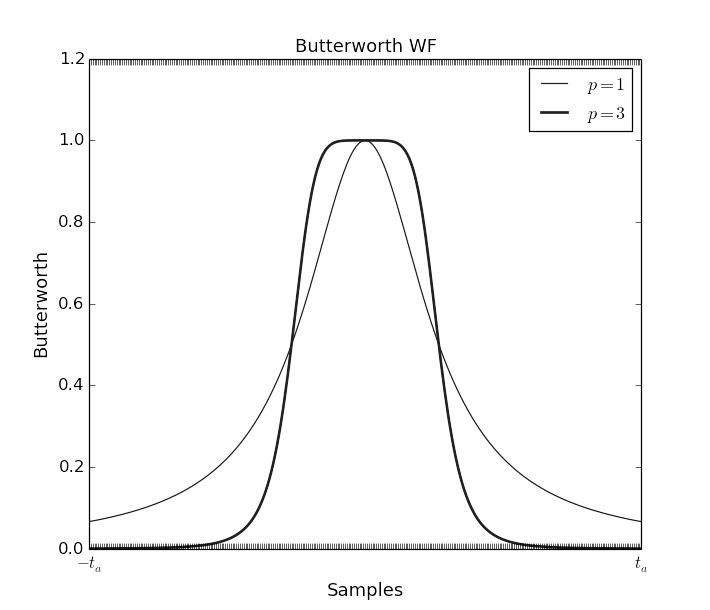
\includegraphics[width=.5\textwidth]{./Figures/butterworthgrey.png}%
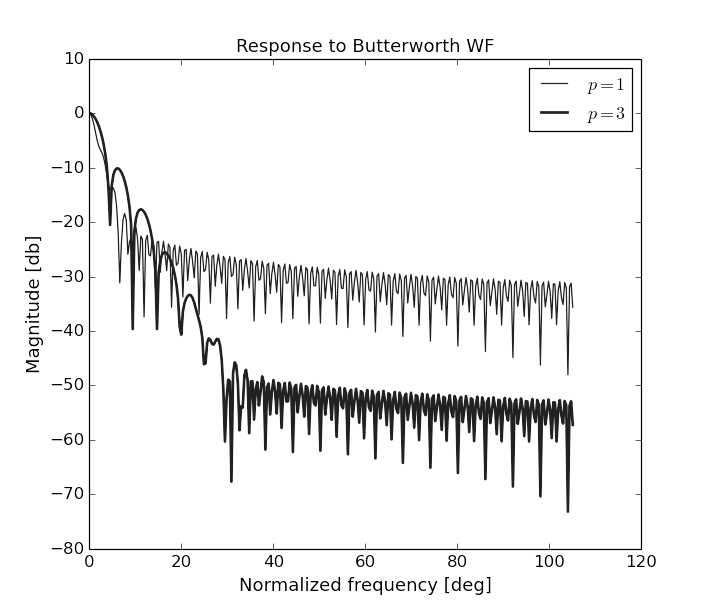
\includegraphics[width=.5\textwidth]{./Figures/freq_resp_butterworthgrey.png}
\caption{Butterworth windowing function and its tapering response.}\label{fig:wf:bw}
\end{figure*}

A Butterworth WF is flat in the time pass band, and rolls off towards zero in the time stop band and it is 
characterized by two independent parameters, the cut-off time time $[-t_a,t_a]$ and the order $p$. 
The two parameters control the 
FoV and sidelobes attenuation. The Butterworth WF is given by:
\begin{equation}
BW(t)= \Pi(t) \Big(1 + (t/t_a)^{2p}\Big)^{-1}.
\end{equation}

Figure \ref{fig:wf:bw} shows Butterworth WFs for the same cut-off interval $[-t_a,t_a]$, with orders of $p=1,3$. Note that increasing 
the order $p$ conserves the MLW, and dramatically lowers distant sidelobes, at the cost of pushing up the near-in sidelobes

\subsection{Sinc window}
\begin{figure*}
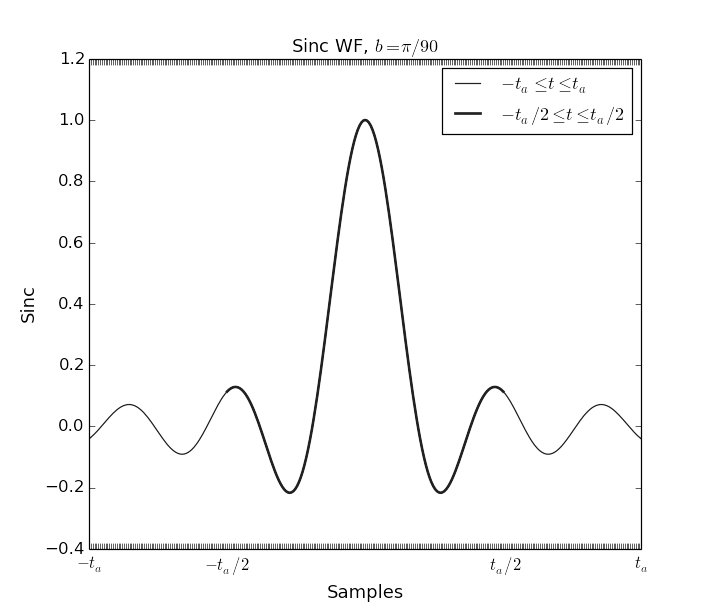
\includegraphics[width=.5\textwidth]{./Figures/sincgrey.png}%
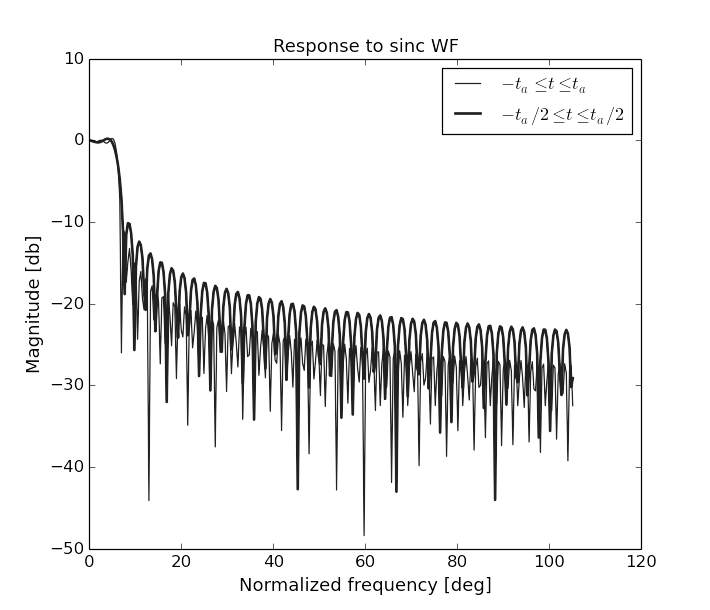
\includegraphics[width=.5\textwidth]{./Figures/freq_resp_sincgrey.png}
\caption{Sinc windowing function and its tapering response.}\label{fig:wf:sinc}
\end{figure*}
The sinc WF is defined as 
\begin{equation}
S(t)= \Pi(t) \frac{\sin(\pi b t)}{\pi b t} .
\end{equation}
Fig. \ref{fig:wf:sinc} shows $S(t)$ for a fixed value of $b$, and cut-off intervals given by $[-t_a,t_a]$ and $[-t_a/2,t_a/2]$.
Note that the response to a sinc WF is almost perfectly flat in the main lobe (more so for larger intervals). The sidelobe response is relatively poor, but better for larger intervals.

\subsection{Bessel $J_0$ window}
\label{Bessel}
\begin{figure*}
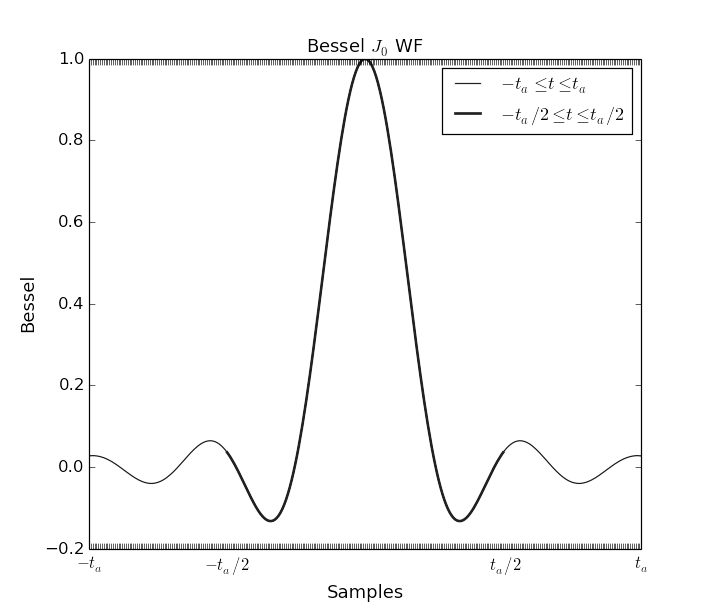
\includegraphics[width=.5\textwidth]{./Figures/besselgrey.png}%
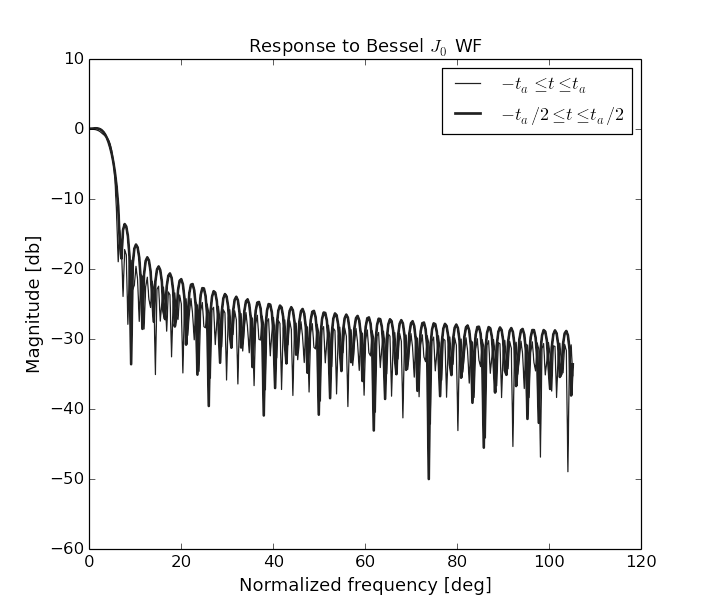
\includegraphics[width=.5\textwidth]{./Figures/freq_resp_besselgrey.png}
\caption{Bessel (of the first kind) windowing function and its tapering response.}\label{fig:wf:bessel}
\end{figure*}


This WF is given by a Bessel function of the first kind of order zero. Using a power series expansion, we have:
\begin{equation}
J_0(t) = \Pi(t) \sum_{k=0}^{\infty}\frac{(-1)^k (t/2)^{2k}}{(k!)^2}
\end{equation}
Fig. \ref{fig:wf:bessel} shows J$_0(t)$ and its response, with $J_0(t)$ truncated at time intervals $[-t_a,t_a]$ and 
$[-t_a/2,t_a/2]$. The performance of $J_0$ is somewhat worse than the sinc within the main lobe, and somewhat better in
the sidelobes.

\subsection{Prolate spheroidal wave $PS_{0}$ window}
\begin{figure*}
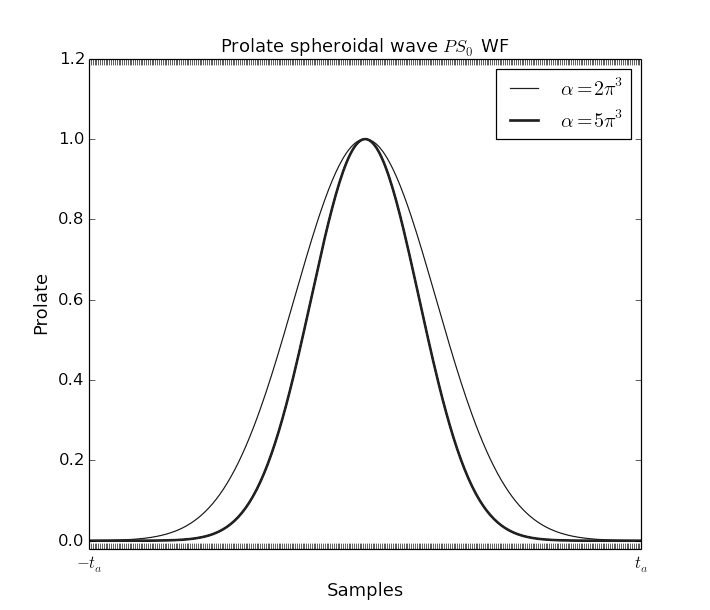
\includegraphics[width=.5\textwidth]{./Figures/prolategrey.png}%
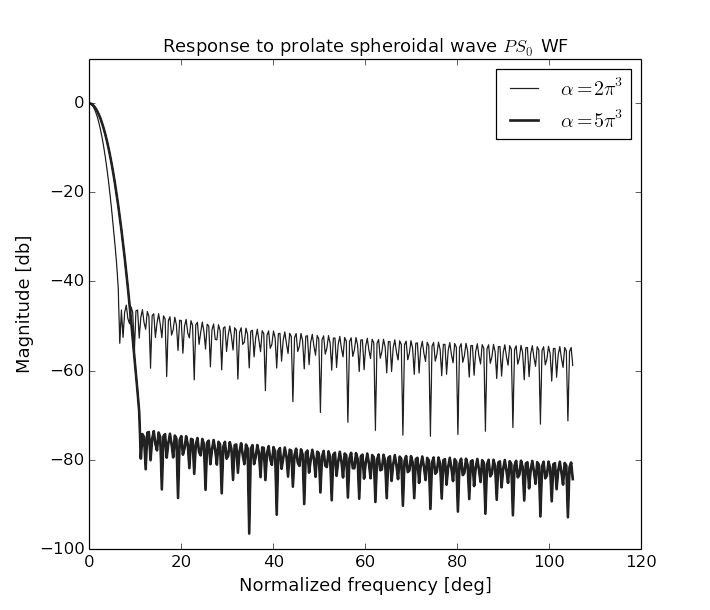
\includegraphics[width=.5\textwidth]{./Figures/freq_resp_prolategrey.png}
\caption{Prolate spheroidal wave (of oder zeros) windowing function and its tapering response.}\label{fig:wf:prolate}
\end{figure*}
This WF is given by a prolate spheroidal wave function of sequence zero ($n=0$) characterized
by two independent parameters, the cut-off time $[-t_a,t_a]$ and the order $\alpha$ 
\citep{landau1978prolate,delsarte1985discrete}. 
The two parameters control the  FoV and sidelobes attenuation.
The prolate spheroidal wave $PS_0$ is the eigen function and solution of the integral :
\begin{equation}
\int_{-t_a}^{t_a} PS_{0}(\xi) \frac{sin(\frac{\alpha}{\pi}(t-\xi))}{\frac{\alpha}{\pi}(t-\xi)}d\xi=\lambda_{n=0,\alpha,t_a}PS_{0}(t), 
 \end{equation}
where $\lambda_{n=0,\alpha,t_a}$ is the eigen value of the prolate spheroidal wave $PS_{0}(t)$ WF.
Fig. \ref{fig:wf:prolate} shows prolate spheroidal wave $PS_0(t)$ WFs for the same cut-off interval $[-t_a,t_a]$, 
with orders of $\alpha=2\pi^3, 5\pi^3$. Note that increasing 
the order $\alpha$ increases the MLW, and dramatically lowers sidelobes.

\subsection{$J_0$-Hamming, $J_0$-Hanning and $J_0$-Blackman windows}
\begin{figure*}
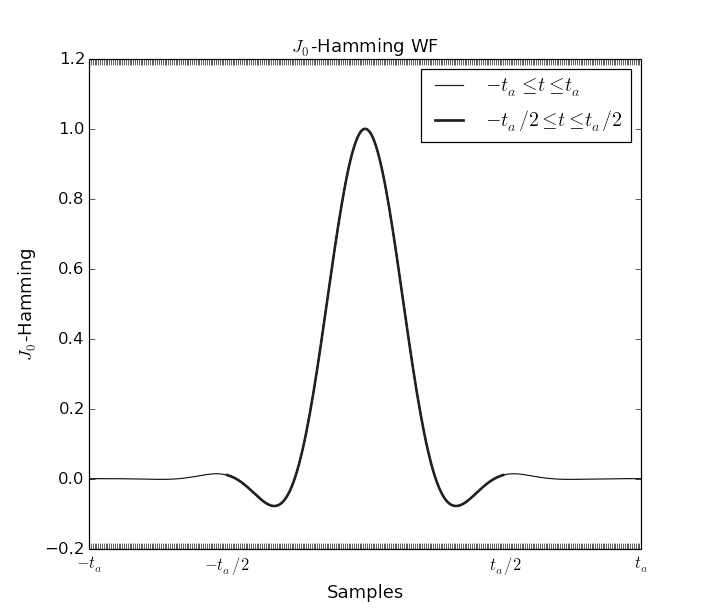
\includegraphics[width=.5\textwidth]{./Figures/bessel-hamminggrey.png}%
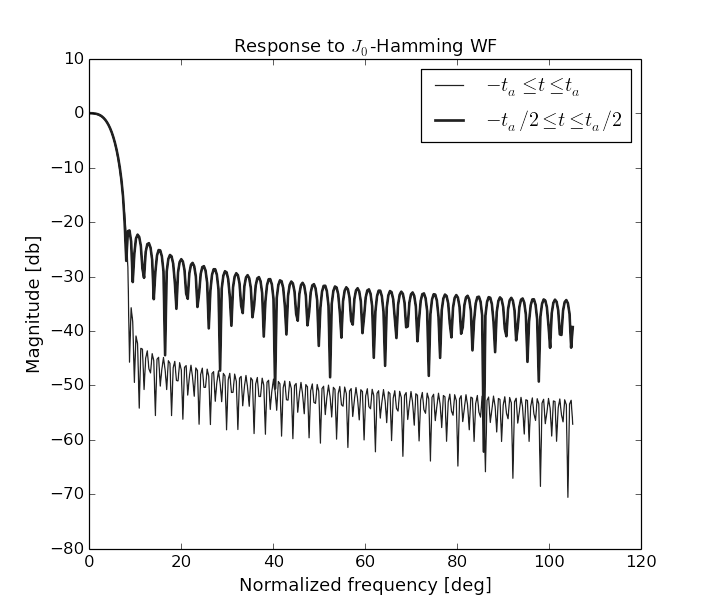
\includegraphics[width=.5\textwidth]{./Figures/freq_resp_bessel-hamminggrey.png}
\caption{Prolate spheroidal wave (of oder zeros) windowing function and its tapering response.}\label{fig:wf:bessel-ham}
\end{figure*}
\begin{figure*}
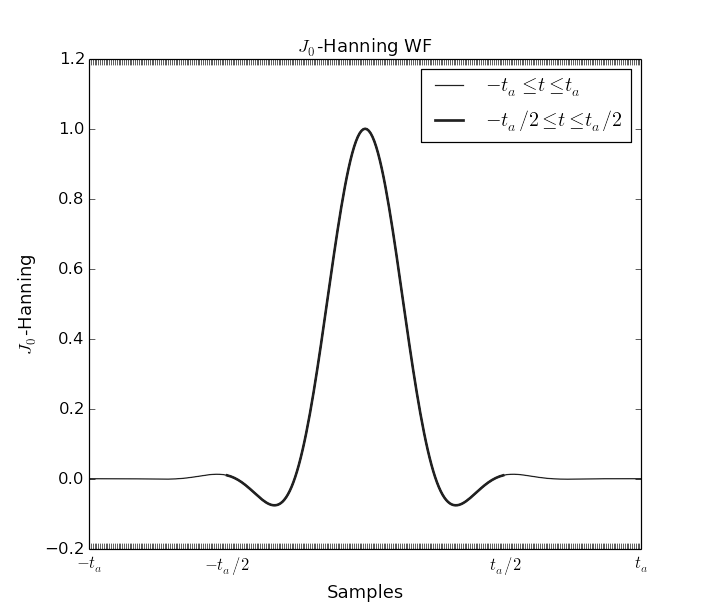
\includegraphics[width=.5\textwidth]{./Figures/bessel-hanninggrey.png}%
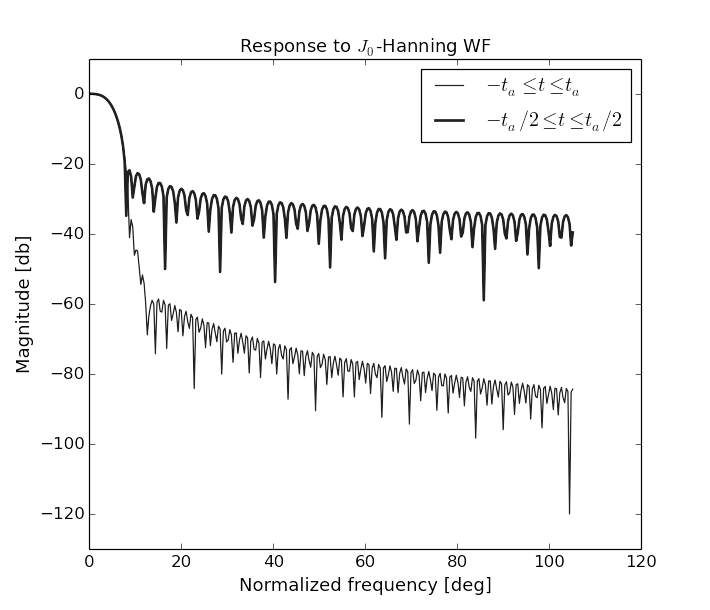
\includegraphics[width=.5\textwidth]{./Figures/freq_resp_bessel-hanninggrey.png}
\caption{Prolate spheroidal wave (of oder zeros) windowing function and its tapering response.}\label{fig:wf:bessel-han}
\end{figure*}
\begin{figure*}
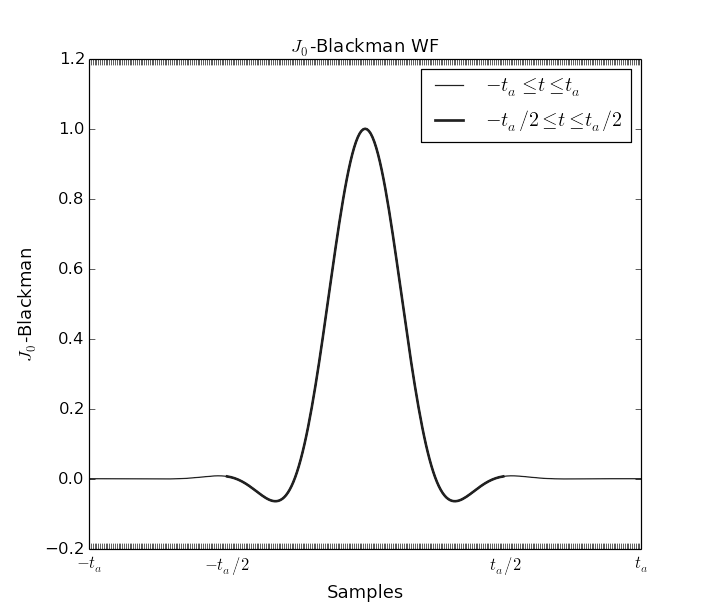
\includegraphics[width=.5\textwidth]{./Figures/bessel-blackmangrey.png}%
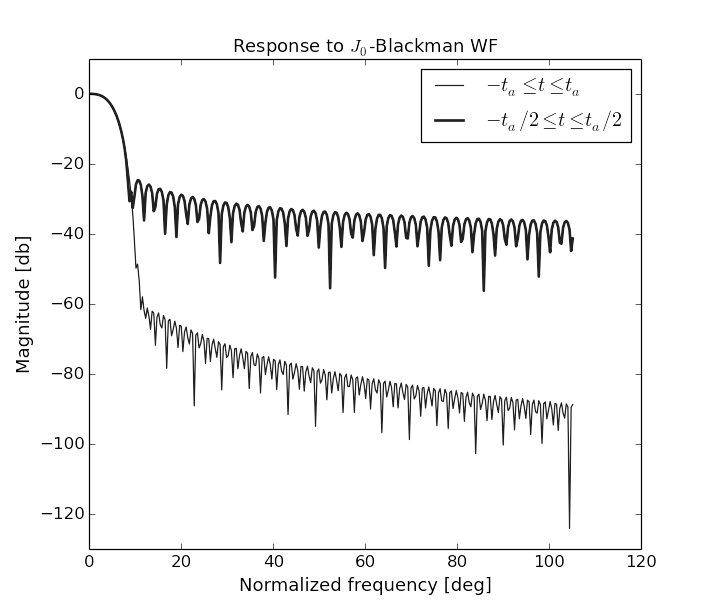
\includegraphics[width=.5\textwidth]{./Figures/freq_resp_bessel-blackmangrey.png}
\caption{Prolate spheroidal wave (of oder zeros) windowing function and its tapering response.}\label{fig:wf:bessel-black}
\end{figure*}
A $J_0(t)$ WF can be used to filter out the input signal, providing an intermediate signal. The intermediate signal 
can then be passed through a Hamming, Hanning or Blackman filter to further increase the pass band (regime 1 or FoV) and 
increase the stop band (regime 3 or outside the FoV) attenuation. The process can be resume as follow:
\begin{equation}
BX(t)= J_0(t)X(t) 
\end{equation}
where $X(t)$ is either the Hamming or the Hanning or the Blackman WFs known in the litterature.
Fig. \ref{fig:wf:bessel-ham}, Fig. \ref{fig:wf:bessel-han} and Fig. \ref{fig:wf:bessel-black}  show $BX(t)$ WFs and their
response with the Hamming, Hanning and Blakman respectively. Compare to the $J_0(t)$ WF, the $BX(t)$ has lower PSL and higher SLR.

\subsection{Relative performance}
% \subsection{Convolution theorem and WFs comparison}
% We begin with a continuous signal $V_{t}$ (supposed the data is only time dependent) and sample it in order to obtain the set of 
% measurement (see section \ref{sec:AvgCon}). When the signal is limited in the time interval $[-t_a,t_a]$ and convolved with a window 
% $W_{t}$, it 
% follows from the convolution theorem that the process was equivalent to "\textit{tapering the  Fourier transform of the signal}" by 
% effectively looking at the true Fourier transform of the signal through the convolution window. This is presented mathematically as:
% \begin{equation}
% \mathcal{F}\Big\{V_{t}\circ W_{t}\Big\} = \mathcal{F}\Big\{V_{t}\Big\}\cdot \mathcal{F}\Big\{W_{t}\Big\}
% \end{equation}
% One can replaced the convolution window, $W_{t}$ by its Fourier transform. A summary of the MLW, the PSL and 
% the SLR of the windows study is showed in table below.
\begin{table}
\begin{tabular}{|l||l|l|l|l|}
\hline
 \bf WFs& &\bf{Windows} & \bf response\\
 &&{ MLW} & { PSL}  & { SLR}   \\
  &&\hspace{-0.8cm}(deg and at -3db) & (db) & (db/oct)  \\
\hline\hline
{$\Pi(t)$}  & $t\in|t_a|$& $\sim 1.406$ &$-6.663$ &$-12.089$\\
	    & $t\in|t_a/2|$&$\sim 2.812$ &$-6.671$ &$-11.065$\\
\hline
{$S(t)$} & $t\in|t_a|$ &$\sim 12.304$& $-10.889$&  $-12.661$ \\
	 & $t\in|t_a/2|$ &$\sim 12.304$& $-13.241$&  $-11.447$ \\
\hline
{$J_0(t)$}& $t\in|t_a|$ &$\sim 9.140$ &$ -14.553$ & $ -12.011$\\
	  & $t\in|t_a/2|$ &$\sim 9.140$ &$ -13.614$ & $ -11.794$\\
\hline
{$G(t)$} & b=3 &$\sim 2.109$& $-21.535$& $-9.589$\\ 
	 & b=5 &$\sim 2.812$& $-30.211$& $-9.091$\\ 
\hline
{$BW(t)$} & p=1 &$\sim 2.109$ &$-13.718$ & $-12.581$\\
	  & p=3 &$\sim 4.218$ &$-10.145$ & $-27.330$\\
\hline
{$PS_0(t)$} & $\alpha=2\pi^3$ &$\sim 3.515$& $-45.302$& $-7.424$\\ 
	 & $\alpha=5\pi^3$ &$\sim 4.218$& $-73.597$& $-6.375$\\ 
\hline
{$BX(t)$} & $t\in|t_a|$ &$\sim 9.140$&$-35.724$ & $-11.948$\\ 
{$Hamming$}	 & $t\in|t_a/2|$ &$\sim 9.140$&$-22.670$&$-19.527$\\ 
\hline
{$BX(t)$}   & $t\in|t_a|$ &$\sim 9.140$&$-35.954$ &$-41.684$ \\ 
{$Hanning$}   &$t\in|t_a/2|$ &$\sim 9.140 $&$-27.765$&$-46.233$\\ 
\hline
{$BX(t)$}  & $t\in|t_a/2|$ &$\sim 9.140$&$-48.660$&$-37.274$\\ 
{$Blackman$}	 & $t\in|t_a/2|$ &$\sim 9.140$&$-24.723$&$-7.972$
\end{tabular}
\caption{\label{tab:WF:performance}Comparative performance of 
different windowing functions. 
\bf{OMS: Marcellin, it is not clear what exact variation of the
WF these numbers correspond to. Maybe add a few rows for different variations (i.e. different values
of $p$, $b$)? In fact, it's not even clear if the comparison is systematic. For example, the FoV realized 
by different WFs is different.}
\emph{ Marcellin anwser, thank you I noticed that when I was doing the new plots, I'll do it explicitly and 
I want to change the scaling of the windows so that we can easily see what you are asking.}}
\end{table}
Table~\ref{tab:WF:performance} summarizes the performance of the different WFs. From this it is clear that
the sinc, the Butterworth (BW) and the Bessel ($J_0$) WFs provide the more optimal tapering response. It is these WFs that
will serve as the basis of BDWFs developed in the rest of this work. 

To construct two-dimensional BDWFs from one-dimensional WFs, we will use the following definitions:
\begin{eqnarray}
S(u,v) &=& S(u)S(v), \nonumber\\
J_0(u,v) &=& J_0(r), \nonumber\\
BW(u,v) &=& BW(r),~~~r=\sqrt{u^2+v^2}.
\end{eqnarray}

{\bf OMS: Marcellin, why not $\mathrm{sinc}(r)$ as well? The referee is bound to ask? Also, why did you never consider a 
prolate spheroidal WF? I remember bringing it up a few times.}\\
{\bf Marcellin: $\mathrm{sinc}(r)$ dosn't works well in signal recovery. I studied the prolate spheroidal wave functions(PSWF)
and the oder 1 of PSWF was just slightly like the sinc but with low sidelobes. I can try and test this but for sure 
the computational time is extremely huge. I was thinking to talk about 
the Hamming*[sinc or bessel], Hinning*[sinc or bessel], blackman*[sinc or bessel] there are also performing well.}


\section{Application of WFs to visibilities}

While visibilities are (usually) regularly sampled in $t\nu$-space, in $uv^\mathrm{m}$-space this is not so. In frequency the sampling
positions go as $\sim\nu^{-1}$, while in time, baselines with a longer East-West component sweep out longer tracks between successive 
integrations (Fig.~\ref{fig:uvcov}). Applying a WF with a constant integration window in $t\nu$ space corresponds to 
different-sized windows in $uv$-space. In the case of normal averaging, this results in the boxcar-like window $\Pi^\prime$ of 
eq.~(\ref{eq:avscon}) having a baseline-dependent scale. The scale of the tapering response being inversely proportional to 
the scale of the WF, this results in more smearing (i.e. a narrower taper) on longer baselines.

By defining our alternative WFs in $uv$-space (in units of wavelength), we can attempt to ``even out'' the smearing 
response across baselines. For example, adopting a Bessel windowing function $J_0(u,v)$, we have the following recipe 
for computing averaged visibilities:
\begin{equation}
\label{eq:avg:bessel}
V^\mathrm{(m)}_{pqkl} = \frac{\sum\limits_{{i,j}\in B_{kl}} \VV_{pq}(\bmath{u}_{ij}) J_0(\bmath{u}_{ij}-\bmath{u}_{kl})}
{\sum\limits_{i=k_0}^{k_1} \sum\limits_{{i,j}\in B_{kl}} J_0(\bmath{u}_{ij}-\bmath{u}_{kl})},
\end{equation}
where $B_{kl}=[k_0\dots k_1]\times[l_0\dots l_1] $ represents the sample indices being averaged over, and
$\bmath{u}_{kl}$ is the midpoint of the bin. The effective WF is therefore scaled by the baseline fringe rate, and 
truncated at the edges of the averaging interval. On the shortest baselines, the truncation is extreme to the point of 
approaching the boxcar-like $\Pi^\prime$ (Fig.~\ref{fig:WF:perbaseline}).

\begin{figure*}%
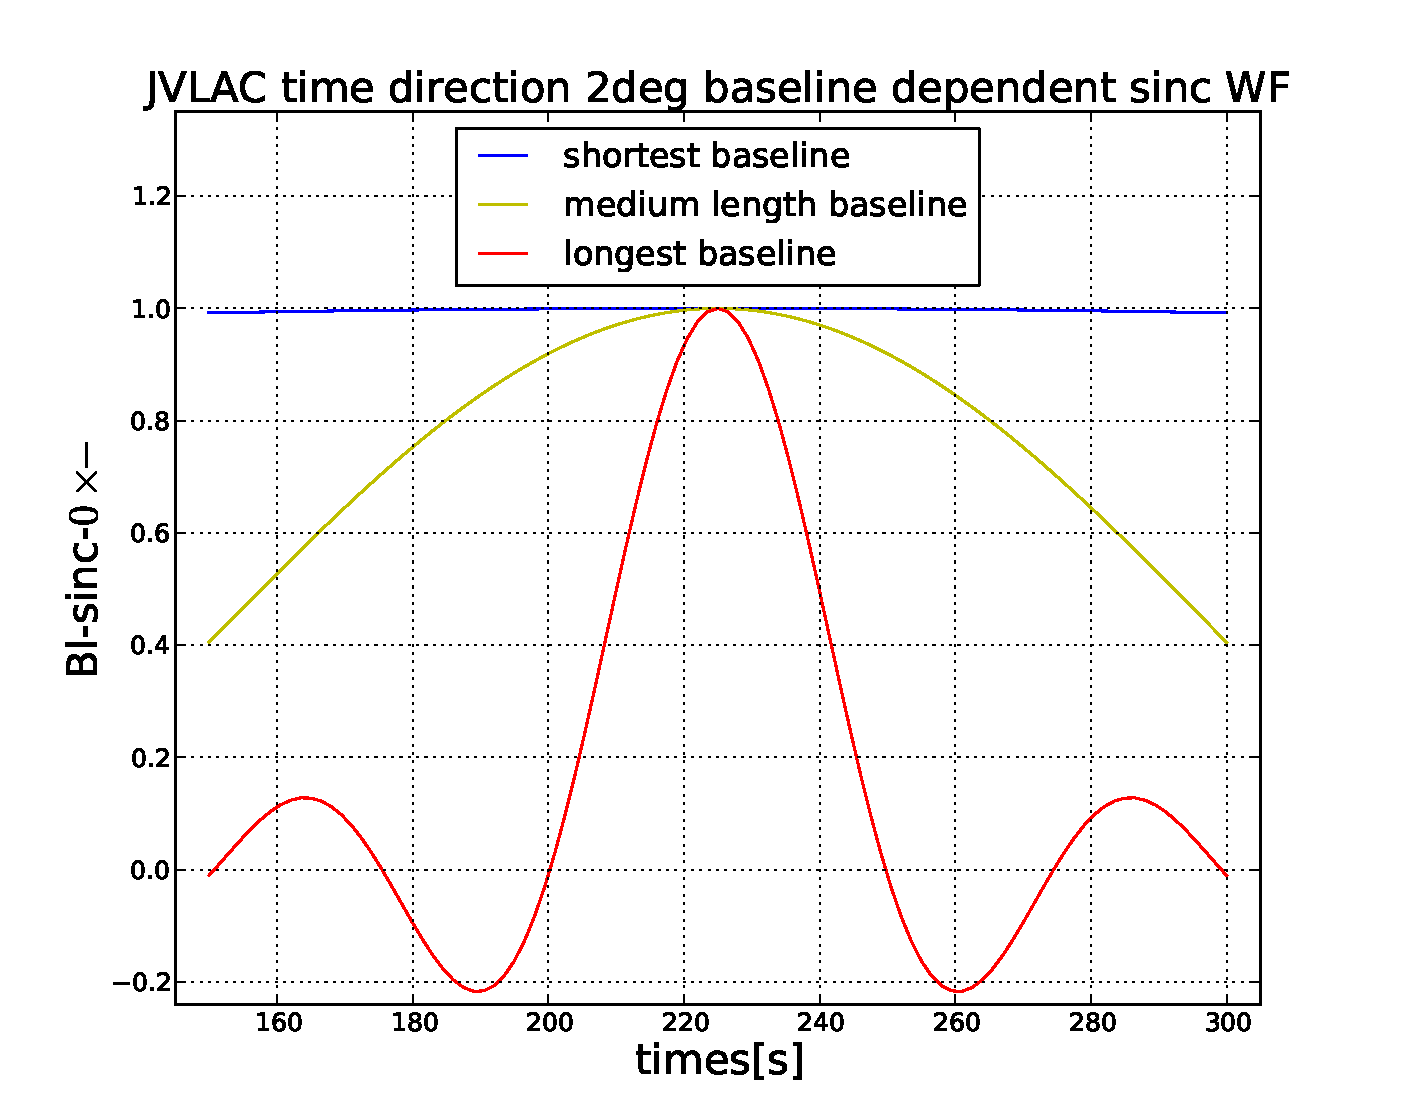
\includegraphics[width=.33\textwidth]{./Figures/longshortmid-sinc.pdf}\hfill%
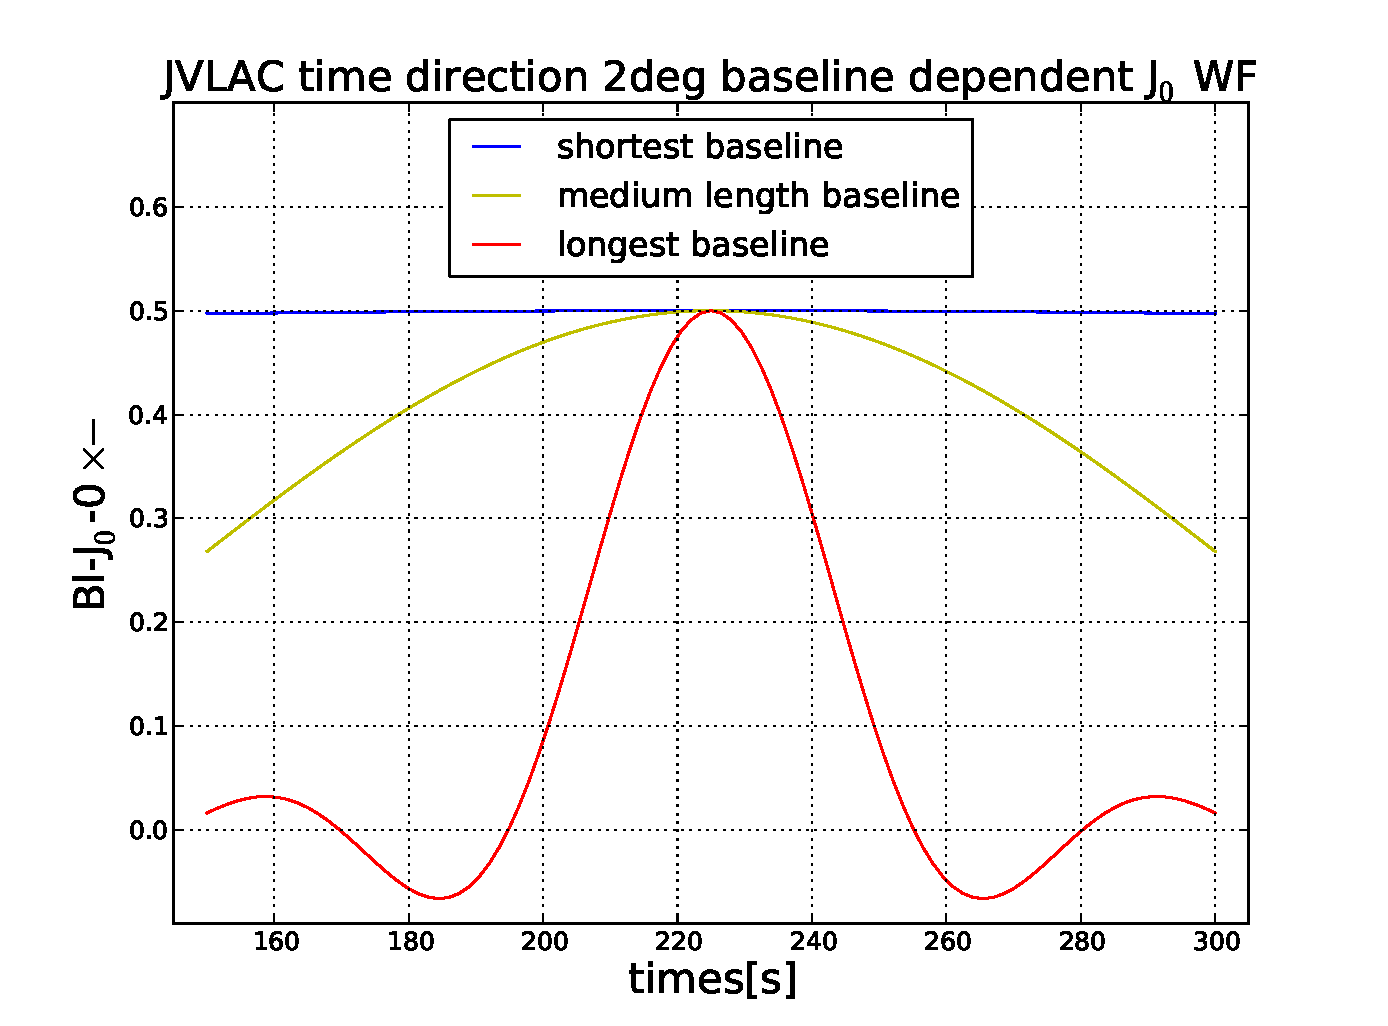
\includegraphics[width=.33\textwidth]{./Figures/longshortmid-bessel.pdf}\hfill%
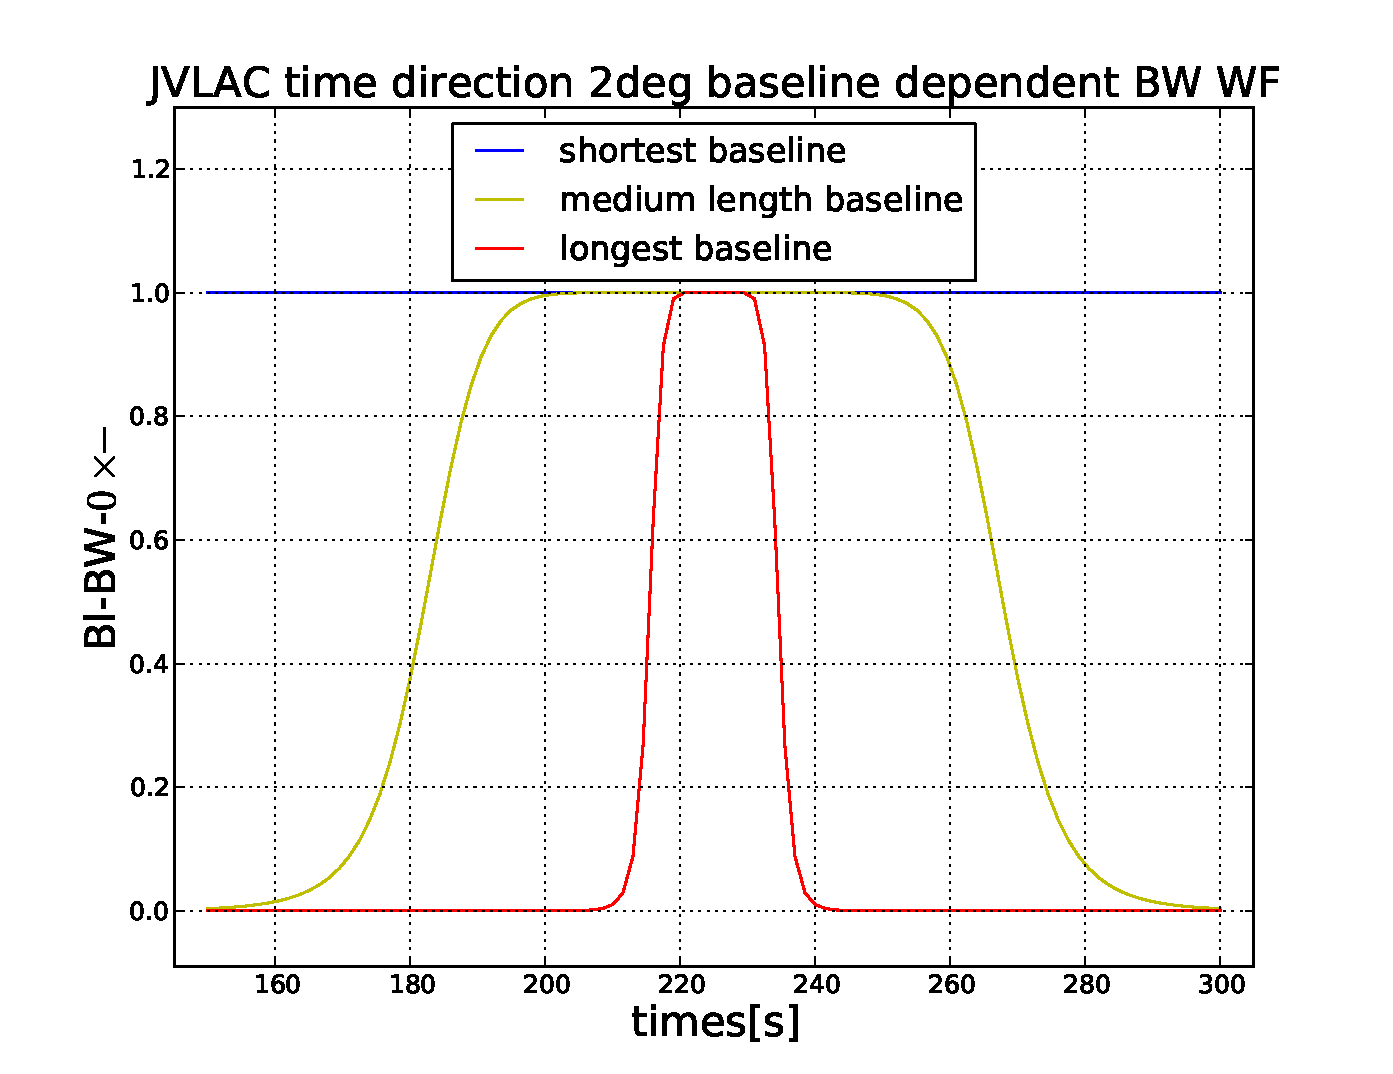
\includegraphics[width=.33\textwidth]{./Figures/longshortmid-butter.pdf}
\caption{Cross-sections through three different BDWFs (left: sinc, centre: Bessel, right: Butterworth) defined in $uv$-space, 
plotted along the time axis. This shows that the effective WF is a scaling and truncation of the underlying WF, with
the shortest baselines reducing to a boxcar-like WF.}
\label{fig:WF:perbaseline}
\end{figure*}

The downside of this simple approach is twofold. Firstly, while all of the WFs above boast far lower sidelobes than the boxcar
(i.e. more suppression for out-of-FoV sources), they no longer perform that well under truncation, with extremely truncated WFs 
at the shorter baselines becoming boxcar-like. Secondly, taking a weighted sum in eq.~\ref{eq:avg:bessel} increases 
the noise in comparison to normal averaging.

\subsection{Overlapping BDWFs}
\label{baseline2}

A more sophisticated approach involves overlapping BDWFs. Normal averaging implicitly assumes that the averaging bins $B_{kl}$ 
in eq.~\ref{eq:avg:bessel} don't overlap, since they represent adjacent averaging intervals. There is, however, no reason 
(apart from computational load) why we cannot enlarge the bins so that the averaging intervals actually overlap by 
some number of samples. For normal averaging this makes little sense, since it effectively broadens $\Pi^\prime$ and therefore
increases smearing. But for a well-behaved BDWF, enlarging the window (while maintaining the same WF scale) means 
less truncation -- thus lower sidelobes -- and decreased noise, as more samples are taken into account.



In theory, WFs and signals generally extend to  infinity. Unfortunately, in practice, filtering a signal with a low pass 
filter, one need to define a cut-off interval (range of uv-bins). Therefore, if one  wants to achieve sufficiently an accurate  estimate 
of the WF ideal image plane response (IPR), one need a wide cut-off interval as far as the IPR approaches 
the ideal when the WF order increases. An overlap BDWF aims to extend the order of the BDWF in 
such a way that, we approach the ideal IPR. The only drawback of this technique is the increase in time needed for processing the 
output sample of the signals being integrate.

The weight of a uv-bin is not defined by a unique BDWF but by the 
strength of the correlation between the overall  overlapping BDWF as shown in Figure \ref{fig:corrSigVLAMxBl_overlapGdelta}. 
That said, the weight of a uv-bin becomes the summation of overlapping BDWF samples on the uv-bin normalized by the summation of the 
overall uv-bins weights within the range where the overlap samples are defined.
\begin{figure} 
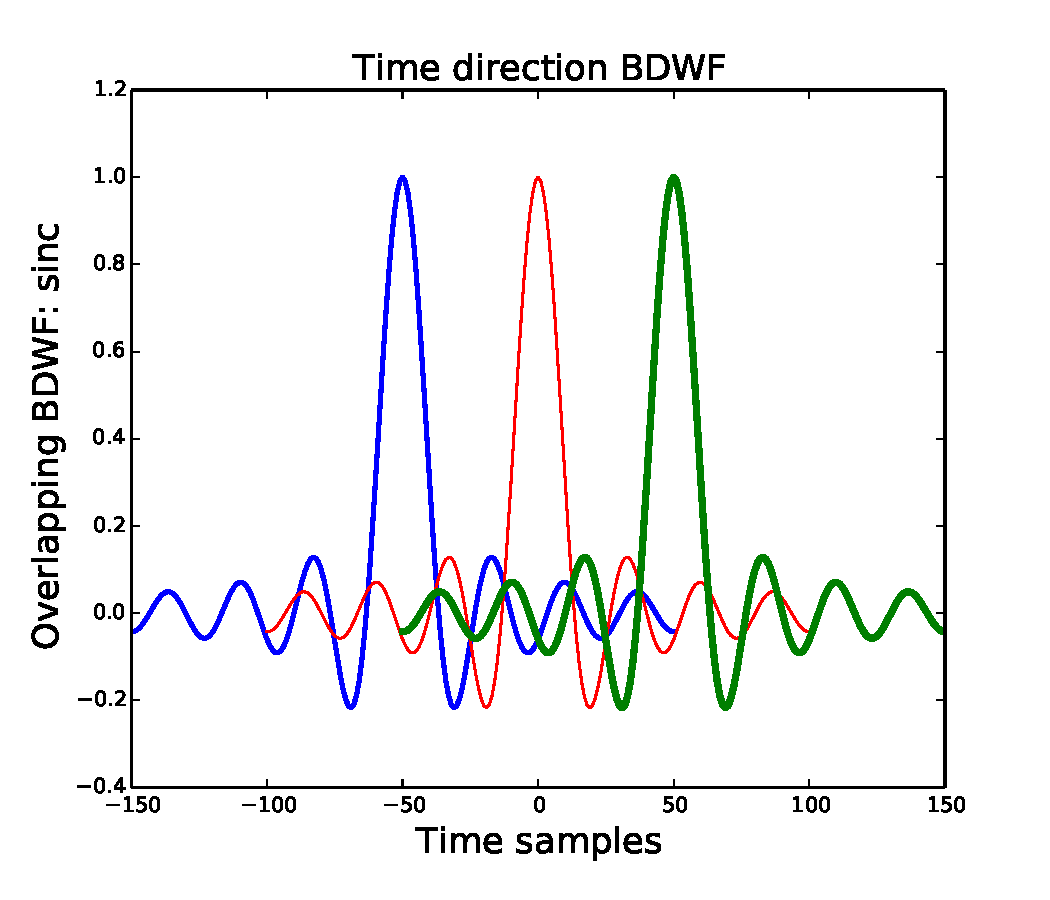
\includegraphics[width=1\columnwidth]{./Figures/corrSigVLAMxBl_overlapGdelta.pdf}\caption{Overlap 
baseline dependent windowing functions}\label{fig:corrSigVLAMxBl_overlapGdelta}
\end{figure}
%Now, consider that $f^{a}_{pq}$ is an overlap-\textit{BDWF} 
%of width  $\Delta t$ and $\Delta \nu$ across the time and frequency direction respectively.
% \begin{definition}[Left hand side overlapping functions]
% \label{def:4}
% if $\Delta_l t$ and $\Delta_l \nu$ are the overlap time interval and frequency interval of the baseline dependent windowing function  
% $f_{pq}^{a_0}$ respectively  and $\Big\{f_{pq}^{a_1},f_{pq}^{a_2},f_{pq}^{a_3}, \dots \Big\}$ the set of \textit{BDWF} overlapping  on the 
% \textit{left hand side} of $f_{pq}^{a_0}$ then the resulting \textit{BDWF} within $\Delta_l t$ and $\Delta_l \nu$ is defined as
% \begin{eqnarray*}
%  g^{lhs}_{pq}: \{\mathbf{\mathcal{R}},\mathbf{\mathcal{R}}\} &\rightarrow& \mathbf{\mathcal{R}}\\
%                    d_{t_i},d_{\nu_j} &\mapsto& \frac{1}{N_{lhs}}\Bigg(\sum_{k}f_{pq,(d_{t_i},d_{\nu_j})}^{a_k} 
% + f_{pq,(d_{t_i},d_{\nu_j})}^{a_0}\Bigg).
% \end{eqnarray*}
% Here, $N_{lhs}$ is the normalization term defined as
% \begin{eqnarray*}
% N_{lhs}=\sum_{i=1}^{n_{lt}}\sum_{j=1}^{n_{l\nu}}\Bigg(\sum_{k}f_{pq,(d_{t_i},d_{\nu_j})}^{a_k} + f_{pq,(d_{t_i},d_{\nu_j})}^{a_0} \Bigg),
% \end{eqnarray*}
% where $n_{lt}$ and $n_{l\nu}$ are the number of $(u,v)$ coordinates changes and frequency changes  within $\Delta_l t$ and $\Delta_l \nu$ 
% respectively.
% \end{definition}
% \begin{definition}[Right hand side overlapping functions]
%  \label{def:4}
%  if $\Delta_r t$ and $\Delta_r \nu$ are the overlap time and frequency interval of a \textit{BDWF} $f_{pq}^{a_0}$ 
% respectively and  $\Big\{f_{pq}^{a_1},f_{pq}^{a_2},f_{pq}^{a_3}, \dots \Big\}$ the set of \textit{BDWF} overlapping on the \textit{right 
% hand side} of $f_{pq}^{a_0}$, then the 
% resulting \textit{BDWF} within $\Delta_r t$ and $\Delta_r \nu$ is defined as
% \begin{eqnarray*}
%  g^{rhs}_{pq}: \{\mathbf{\mathcal{R}},\mathbf{\mathcal{R}}\} &\rightarrow& \mathbf{\mathcal{R}}\\
%                    d_{t_i},d_{\nu_j} &\mapsto& 
% \frac{1}{N_{rhs}}\Bigg (f_{pq,(d_{t_i},d_{\nu_j})}^{a_0}+\sum_{k}f_{pq,(d_{t_i},d_{\nu_j})}^{a_k}\Bigg ).
% \end{eqnarray*}
% Here, $N_{rhs}$ is the normalization term defined as
% \begin{eqnarray*}
% N_{rhs}=\sum_{i=1}^{n_{rt}}\sum_{j=1}^{n_{r\nu}}\Bigg(f_{pq,(d_{t_i},d_{\nu_j})}^{a_0} + \sum_{k}f_{pq,(d_{t_i},d_{\nu_j})}^{a_k}\Bigg),
% \end{eqnarray*}
% where $n_{rt}$ and $n_{r\nu}$ are the number of $(u,v)$ coordinates changes and frequency changes  within $\Delta_r t$ and $\Delta_r \nu$ 
% respectively.
% \end{definition}
% \begin{definition}[Overlap baseline dependent windowing functions]
%  \label{def:4}
% If $f_{pq}^{a_0}$ is a baseline dependent windowing function defined within the time interval $\Delta t$ and the frequency interval 
% $\Delta \nu$, $g^{lhs}_{pq}$ the result of the left hand side of $f_{pq}^{a_0}$ overlapping windowing functions within the time interval 
% $\Delta_l t$ and the frequency interval $\Delta_l \nu$, and $g^{rhs}_{pq}$  the result of the right hand side of $f_{pq}^{a_0}$ overlapping 
% windowing functions within the time interval $\Delta_r t$ and the frequency interval 
% $\Delta_r \nu$, then the overlap baseline dependent windowing function within  $\Delta t$ and $\Delta \nu$ is defined as:
% \begin{eqnarray*}
%  g^{}_{pq}: \{\mathbf{\mathcal{R}},\mathbf{\mathcal{R}}\} &\rightarrow& \mathbf{\mathcal{R}}\\
%                    d_{t_i},d_{\nu_j} &\mapsto&
%  \left\{ 
%   \begin{array}{l l}
%     g^{lhs}_{pq} & \quad \text{if $(t_i,\nu_j) \in (\Delta_l t, \Delta_l \nu)$}\\
%     f^{a_0}_{pq} & \quad \text{if $(t_i,\nu_j) \in (\Delta_m t, \Delta_m \nu)$}\\
%     g^{rhs}_{pq}& \quad \text{if $(t_i,\nu_j) \in (\Delta_r t, \Delta_r \nu)$}
%   \end{array} \right.
% \end{eqnarray*}
% \end{definition}
% where $\Delta_m t$ and $\Delta_m \nu$ are $f_{pq}^{a_0}$ uncorrelated time  and frequency interval respectively. From the above 
% definitions, the following derivation is trivial 
% \begin{equation*}
%  \Big\{\Delta t,\hspace{0.17cm}\Delta \nu \Big\}=\Big\{\Delta_l t \cup \Delta_m t \cup \Delta_r t, \hspace{0.17cm}\Delta_l \nu \cup 
% \Delta_m \nu \cup \Delta_r \nu \Big\}.
% \end{equation*}
%  They follow the rules below:
% \begin{eqnarray*}
%  \Delta_m t= \left\{ 
%   \begin{array}{l l}
%      \cup\{t_i\}_{i=s',\hspace{0.1cm} s' \geq s+1}^{e', \hspace{0.1cm}e'\leq e-1} & \quad \text{if $n_{lt}+n_{rt}< n_t$}\\
%       \{t_c\}& \quad \text{if $n_{lt}+n_{rt} = n_t$}\\
%        \emptyset  & \quad \text{otherwise}
%   \end{array} \right.
% \end{eqnarray*}
% and
% \begin{eqnarray*}
%  \Delta_m \nu= \left\{ 
%   \begin{array}{l l}
%      \cup\{\nu_i\}_{i=s',\hspace{0.1cm} s'\geq s+1}^{e', \hspace{0.1cm}e'\leq e-1} & \quad \text{if $n_{l\nu}+n_{r\nu} < n_{\nu}$}\\
%       \{\nu_c\}& \quad \text{if $n_{l\nu}+n_{r\nu} = n_{\nu}$}\\
%        \emptyset  & \quad \text{otherwise}
%   \end{array} \right.
% \end{eqnarray*}




The following designations will be used in the rest of the paper:

Bl-WF-$n_{ovlpt}\times -$: One dimensional BDWF applied across the time direction; WF is one of the window under 
consideration (sinc, J$_0$ and BW) and $2n_{ovlpt}$ is the number of overlap time bins.

Bl-WF-$-\times n_{ovlp\nu}$: One dimensional BDWF applied across the frequency direction with $2n_{ovlp\nu}$ the number of overlap 
frequency bins.

Bl-WF-$n_{ovlpt}\times n_{ovlp\nu}$: Two dimensional BDWF applied across both time and frequency direction.

Bx-avg-$0\times -$: Boxcar averaging applied across the time direction.

Bx-avg-$-\times 0$: Boxcar averaging applied across the frequency direction. 

Bx-avg-$0\times 0$: Boxcar averaging applied across both time and frequency direction.



\subsection{Theoretical noise estimate and simulation noise}
\label{subsec:noise}
 We show in this section that on shorter baselines, the sinc, the J$_0$ and the BW reduce to the Boxcar window. 
Therefore, we effectively applying a hybrid window in the Fourier plane; a Boxcar on the shorter baselines 
and the WF under consideration on the longer baselines (see Figure \ref{fig:longshortmid-sinc}, \ref{fig:longshortmid-bessel} and 
\ref{fig:longshortmid-butter}). We furthermore evaluated the array
theoretical noise ratio, $R_{\sigma}=\epsilon_{ar,oo}^{bd}/\epsilon_{ar,oo}^{bx}$ predicted in Eq.\ref{eq:noise} of a $2^\circ$ BDWF 
averaging  by the one of boxcar averaging and compared the ratio to the simulation one. For the 
analysis we used a JVLAC measurement set (MS) of 7min30s synthesis with a 1.5s
integration time at 1.4Ghz, with 150 channels of width 125kHz. The MS is filled with 1Jy thermal noise. We then processed boxcar 
averaging and BDWF averaging over 1min30s (width of the time integration) and 12500kHz (channel with). Two overlaps BDWF are presented, 
the first overlap over 2min60s across time and 3125kHz across frequency; the second overlap over 3min45s across time and 6250kHz across 
frequency.

\begin{itemize}
 \item In Figure \ref{fig:per-baseline-noise-ratio-sinc}, \ref{fig:per-baseline-noise-ratio-bessel} 
and \ref{fig:per-baseline-noise-ratio-BW} each \textit{dot mark} is the ratio 
\footnote{$\epsilon^{bd}_{pq,oo}/\epsilon^{bx}_{pq,oo}$, see 
Eq.\ref{eqv:linear} for a recall of $\epsilon^{bd}_{pq,oo}$ and $\epsilon^{bx}_{pq,oo}$.} of per baseline centre pixel theoretical rms 
noise ($\epsilon^{bd}_{pq,oo}$) of a $2^\circ$ BDWF 
averaging  by the one of boxcar averaging ($\epsilon^{bx}_{pq,oo}$). The ratio is plotted as a function of 
$\overline{\mathbf{d}}_t$ (the mean of the baseline $(u,v)$ distance). The figures show that, the noise increases with baseline 
length.
   \item On shorter baselines, the noise estimate of BDWF averaging is approximately the same with the one 
of boxcar averaging. Also, on shorter baselines, the noise drops significantly with the number of  overlap time and frequency bins. As 
mention above, this is because on 
shorter  baselines, the BDWF are closer to the boxcar window, and when the number of overlap time  and 
frequency  bins increases, the ratio:
 $\epsilon^{bd}_{pq,oo}/\epsilon^{bx}_{pq,oo} \approx \sqrt{n_t n_{\nu}/\big((n_t + 2n_{ovlpt})(n_{\nu} + 
2n_{ovlp\nu})\big)}$.%\bigg)^{\frac{1}{2}}
\end{itemize}

The table below summarized the array theoretical rms noise ratio and the simulation one. One do not need to worry about a perfect 
agreement of the theoretical noise results with the simulation one. Unfortunately, the theoretical noise results are the rms noise of the 
sky map centre pixel while the simulation results are an average of the sky map overall pixels rms noise.


\begin{tabular}{*3{c}}
 \multicolumn{3}{|c|}{}\\
\hspace{0.15cm}\begin{tabular}{l*{6}{c}r}
  \hline
  {\bf BDWF} & {\bf Theoretical} & {\bf Simulation}\\
  \hline\hline
  Bl-sinc-0$\times$0 &$1.17$ &$1.23$\\
  Bl-sinc-100$\times$25 &$1.02$ &$1.18$\\
  Bl-sinc-150$\times$50 &$1.03$ &$1.27$\\
  \hline
  Bl-J$_0$-0$\times$0 & $1.11$& $1.14$\\
  Bl-J$_0$-100$\times$25 & $0.91$& $1.08$\\
  Bl-J$_0$-150$\times$50 & $0.92$& $1.13$\\
  \hline
  Bl-BW-0$\times$0 & $1.16$& $1.55$\\
  Bl-BW-100$\times$25 & $1.44$& $1.49$\\
  Bl-BW-150$\times$50 & $1.42$& $1.44$
\end{tabular}
\end{tabular}


\begin{figure*}
    \begin{minipage}{0.38\linewidth}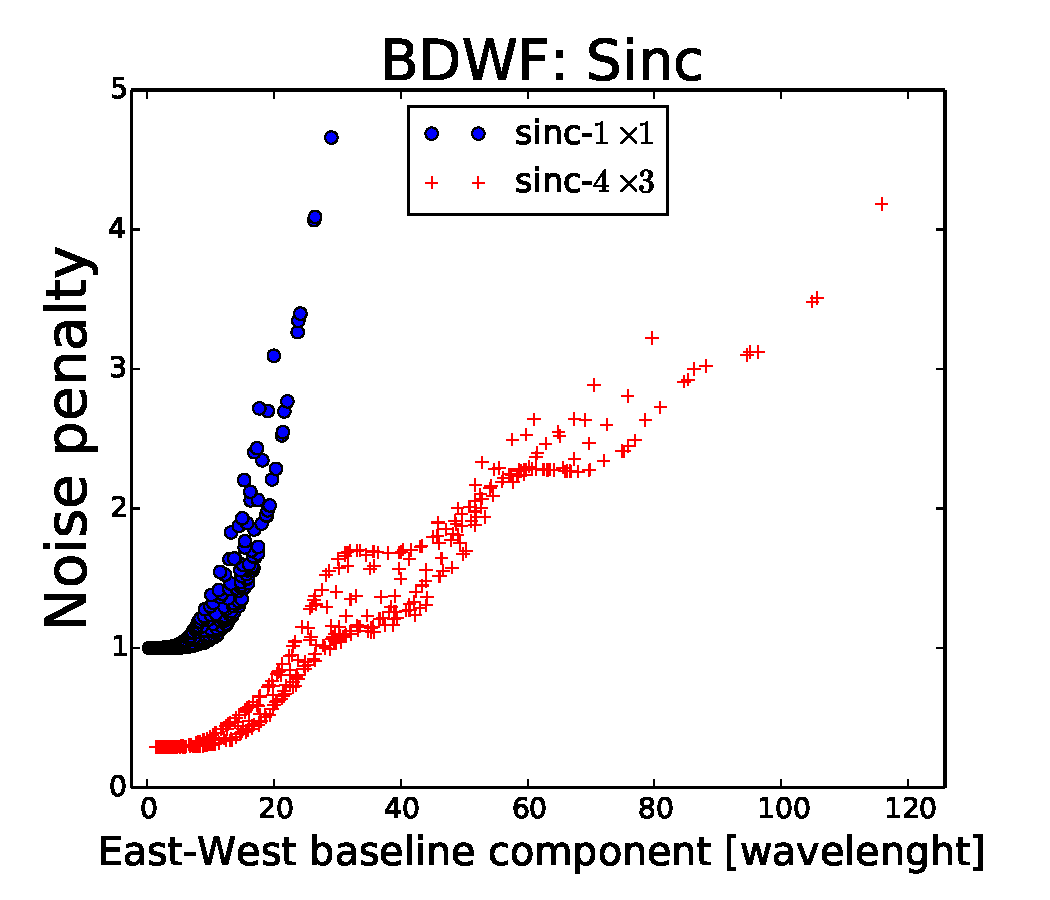
\includegraphics[width=1\textwidth]{./Figures/per-baseline-noise-ratio-sinc.pdf}
  \caption{Per baseline noise ratio of Bl-sinc-W$n_{lt}\times n_{l\nu}$ and averaging}\label{fig:per-baseline-noise-ratio-sinc}
  \end{minipage}
  \hspace{1cm}
  \begin{minipage}{0.38\linewidth}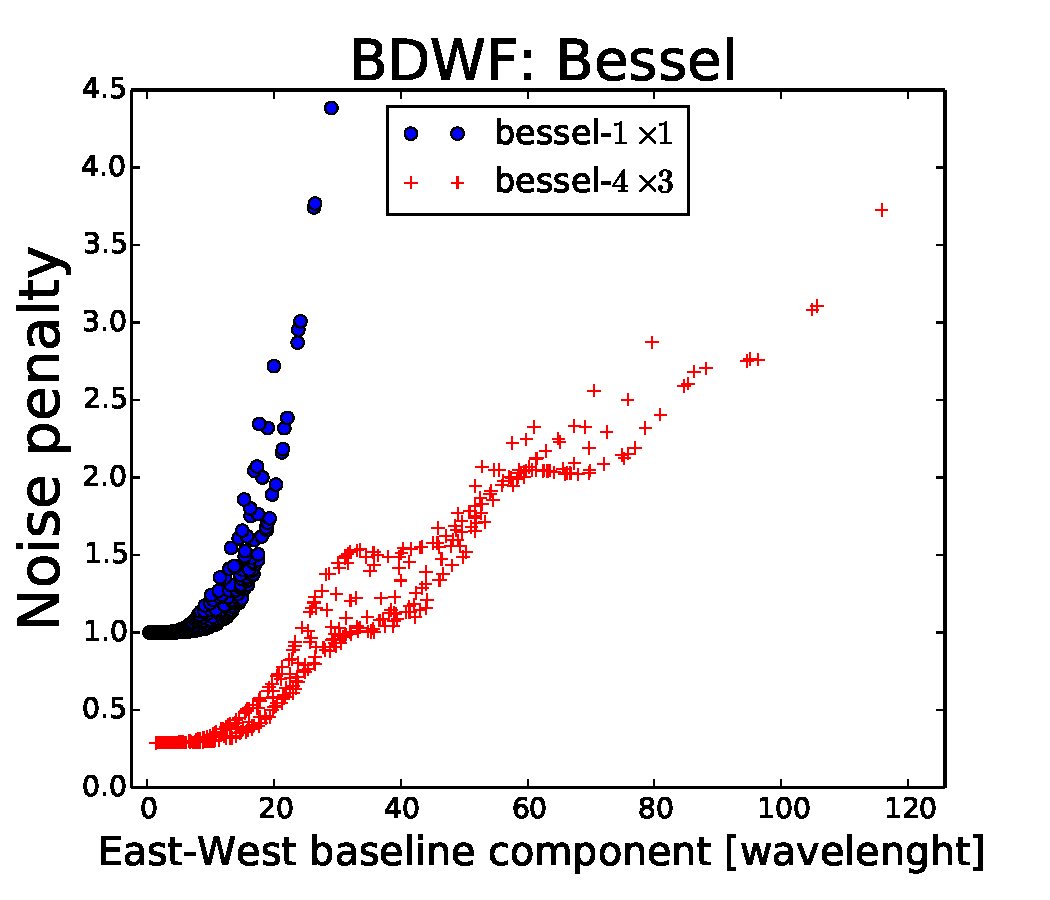
\includegraphics[width=1\textwidth]{./Figures/per-baseline-noise-ratio-bessel.pdf}\\
  \caption{Per baseline noise ratio of Bl-J$_0$-W$n_{lt}\times n_{l\nu}$ and 
averaging}\label{fig:per-baseline-noise-ratio-bessel}\end{minipage}
  \begin{minipage}{0.38\linewidth}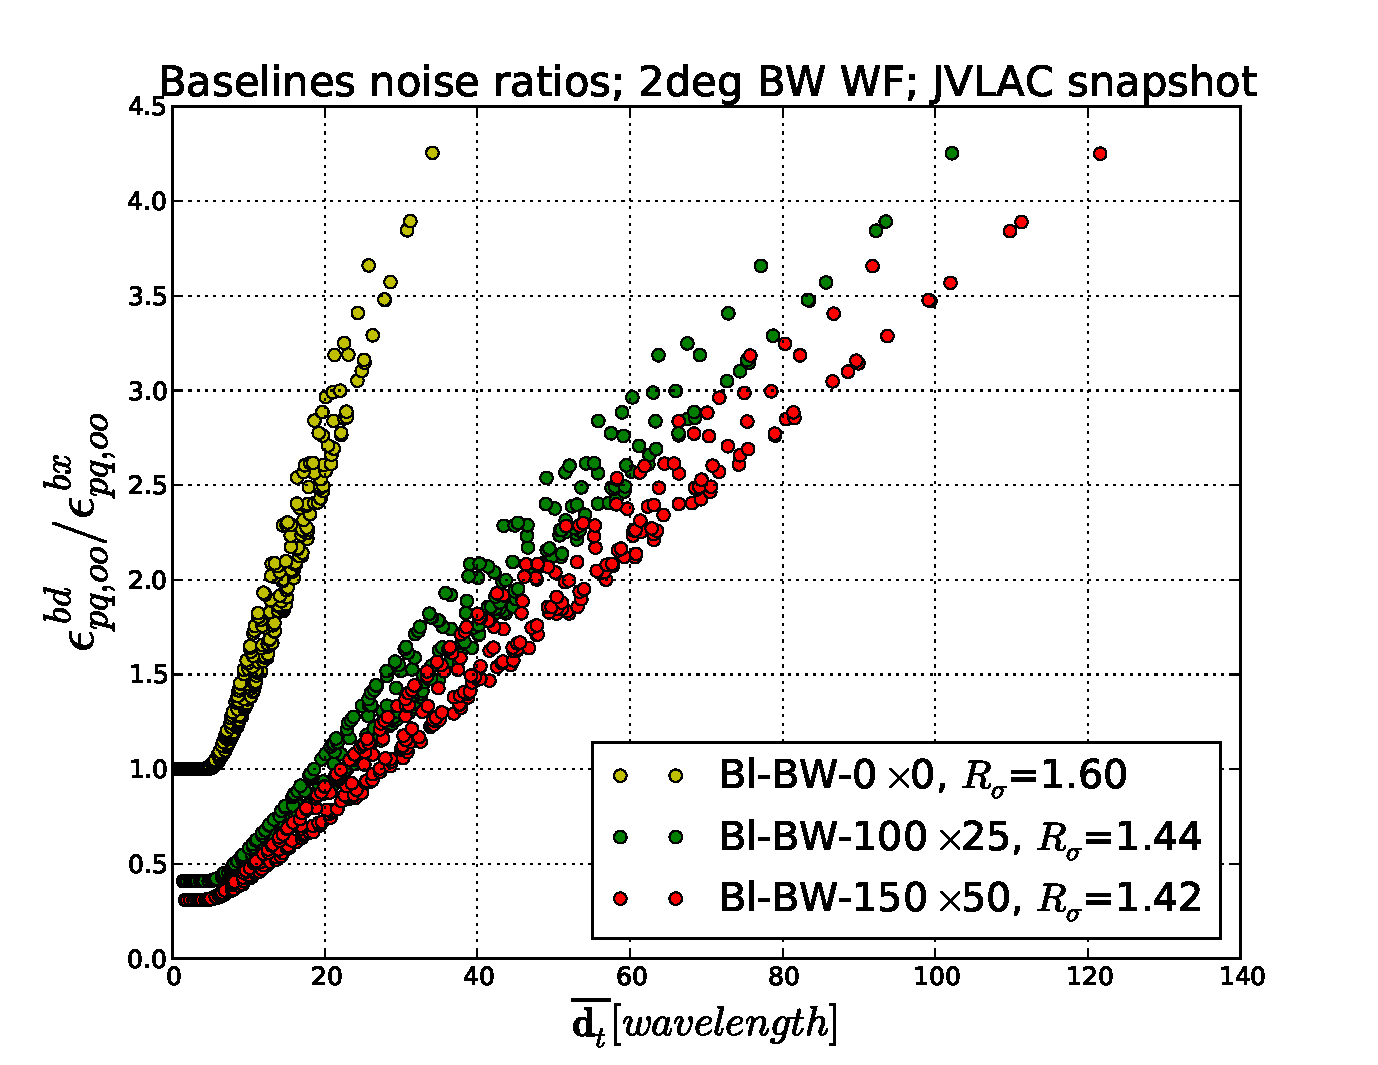
\includegraphics[width=1\textwidth]{./Figures/per-baseline-noise-ratio-BW.pdf}
  \caption{Per baseline noise ratio of Bl-BW-W$n_{lt}\times n_{l\nu}$ and averaging}\label{fig:per-baseline-noise-ratio-BW}
  \end{minipage}
\end{figure*}


\section{Imaging and noise estimate}
\label{sec:imaging}
Recall from the previous section that, the boxcar WF can be replaced by a BDWF, $W_{pq,(t,\nu)}$ that depends 
on $(u,v)$ distances. Now, consider that $\mathcal{\textbf{W}}_{pq,(t,\nu)}$ is  $n_t \times n_{\nu}$ matrix of elements 
$W_{pq,(t_i,\nu_j)}\Big|_{i=1,n_t}^{j=1, n_{\nu}}$, the weights of uv-bins. A uv-bin is a set of four Stocks elements (XX, XY YX, YY) each 
with the same weight $W_{pq,(t_i,\nu_j)}$. Therefore, the sampled visibilities can be presented mathematically as a $4\times n_t\times 
n_{\nu}$ matrix of four polarization times and frequencies dependent matrices each of size $n_t\times n_{\nu}$.
\begin{eqnarray*}
\mathbf{V}_{pq,(t,\nu)}^{samp,i}&=&\Bigg(\mathbf{V}_{pq,(t,\nu)}^{0},\mathbf { V } 
^1_{pq,(t,\nu)},\mathbf{V}^2_{pq,(t,\nu)},\mathbf{V}_{pq,(t,\nu)}^{3 } \Bigg)^{\dagger}, \label{eqx:conv}
\end{eqnarray*}
where the symbol $^{\dagger}$ stand for the transpose operation. The convolution operator is linear, therefore we can re-write Eq.\ref{f4} 
in terms of a series of linear transformations or functional models as:
\begin{equation}
V_{pq,(t_c,\nu_c)}^{corr}= \mathbf{C}_{pq,(t,\nu)}^{block}\cdot\mathbf{W}_{pq,(t,\nu)}^{block}\cdot 
\mathbf{V}_{pq,(t,\nu)}^{samp,i}.\label{eqbb:linear}
\end{equation}
Here, $\mathbf{C}_{pq,(t,\nu)}^{block}$ and $\mathbf{W}_{pq,(t,\nu)}^{block}$ are  blocks diagonals matrices of size $(4n_t 
n_{\nu})\times(4n_t n_{\nu})$, the block elements are $\mathcal{\textbf{W}}_{pq,(t,\nu)}$ and $\mathbf{C}_{pq,(t,\nu)}$ 
respectively, where $\mathbf{C}_{pq,(t,\nu)}$ is the centre time and frequency interval sampling matrix of size $n_t\times 
n_{\nu}$. This
is the result of one time and frequency integration.
For a synthesis, the baseline (p,q) made a complete  coverage in the $(u,v)$ plane. Therefore, we can  
package into a single matrix, $\mathbf{V}_{pq,(t',\nu')}^{corr}$ of size $(4N_t N_{\nu})\times (4N_t N_{\nu})$ the 
BDWF average visibilities of the  baseline (p,q) during the synthesis as follows: 
\begin{equation}
\mathbf{V}_{pq,(t',\nu')}^{corr}=\mathbf{C}_{pq,(t,\nu)}^{block,n_{block}}\cdot 
\mathbf{W}_{pq,(t,\nu)}^{block,n_{block}}\cdot\mathbf{V}_{pq,(t,\nu)}^{samp,n_{block}}.\label{eq2:block}
\end{equation}
The size of 
$\mathbf{V}_{pq,(t',\nu')}^{corr}$ can also be written as $(4N_v^{pq})\times (4N_v^{pq})$, where $N_v^{pq}$ is the total
number of time and frequency visibilities (bins) for the baseline (p,q). The matrices
$\mathbf{C}_{pq,(t,\nu)}^{block,n_{block}}$ and $\mathbf{W}_{pq,(t,\nu)}^{block,n_{block}}$ are diagonals blocks 
matrices of size $(4N_v^{pq}n_t n_{\nu})\times (4N_v^{pq}n_t n_{\nu})$ where each diagonal block is the block diagonal matrix  
$\mathbf{C}_{pq,(t,\nu)}^{block}$ and $\mathbf{W}_{pq,(t,\nu)}^{block}$ respectively. The number of block elements is $n_{block}$. The 
sampled  visibilities 
$\textbf{V}_{pq,(t,\nu)}^{samp,n_{block}}=\mathcal{\textbf{S}}_{pq,(t,\nu)}^{n_{block}}\cdot\mathbf{V}_{pq,(t,\nu)}^{n_{block}}$ is a one 
row matrix of size 
$(N_v^{pq}4 n_t n_{\nu})\times (4 n_t n_{\nu})$ made of $\textbf{V}_{pq,(t,\nu)}^{samp,i}$ on top of each other and the matrix 
$\mathcal{\textbf{S}}_{pq,(t,\nu)}^{n_{block}}$ is the sampling function for the visibilities $\mathbf{V}_{pq,(t,\nu)}^{n_{block}}$ of 
size $(N_v^{pq}4 n_t n_{\nu})\times (4 n_t n_{\nu})$. Note that $i=1,\dots, N_v^{pq}$ and we can write:
\begin{equation}
\mathbf{V}_{pq,(t' \nu')}^{corr}= 
\mathbf{C}_{pq,(t,\nu)}^{block,n_{block}}\cdot\mathbf{W}_{pq,(t,\nu)}^{block,n_{block}}\cdot 
\mathbf{S}_{pq,(t,\nu)}^{n_{block}}\mathbf{F}\cdot\mathcal{I}_{l,m}^{sky }+\epsilon_{pq},\label{eqv:linear}
\end{equation}
our data is always corrupted by a random error component or noise, $\epsilon_{pq}$ (the error component of the baseline (p,q)).
If the number of pixel in the sky model is $N_{pix}$, then the true sky image vector $\mathcal{I}_{l,m}^{sky}$ has a size of $4N_{pix}$ and 
$\textbf{F}$ is a block diagonal Fourier transform operator of size $(4N_{pix})\times(4N_{pix})$.

We are generally interested in using the total set of visibilities over baselines, time and frequencies, having $4\times N_v$ visibilities 
measured over all baselines with $N_v=N_{bl}\times N_v^{pq}$ where $N_{bl}$ is the number of baseline. We then have:\\
\begin{equation}
 \mathbf{V}_{array,(t',\nu')}^{corr}=\mathbf{A}\cdot\mathcal{I}_{l,m}^{sky} + \epsilon. \label{eq:vall}
\end{equation}
 Here, $\epsilon$ is the array error component. $\mathbf{A}$ is a \textit{design} matrix of size 
$(4N_v)\times (4N_{pix})$ designed from $\mathbf{C}_{pq,(t,\nu)}^{block,n_{block}}\cdot \mathbf{W}_{pq,(t,\nu)}^{block,n_{block}}\cdot 
\mathbf{S}_{pq,(t,\nu)}^{n_{block}}\cdot\mathbf{F}\Big|_{p=0,\cdots,n_{a}-1}^{q=p+1,\cdots,n_{a}-1}$ on top of each order, with $n_a$ the 
number of antenna. The \textit{design} matrix is defined as:
\begin{equation*}
\mathbf{A}_{}=
  \begin{bmatrix}
    \mathbf{C}_{01,(t,\nu)}^{block,n_{block}}\cdot \mathbf{W}_{01,(t,\nu)}^{block,n_{block}}\cdot \mathbf{S}_{01,(t,\nu)}^{n_{block}} 
\cdot\mathbf{F}\\
    \vdots\\
    \mathbf{C}_{ik,(t,\nu)}^{block,n_{block}}\cdot \mathbf{W}_{ik,(t,\nu)}^{block,n_{block}}\cdot \mathbf{S}_{ik,(t,\nu)}^{n_{block}} 
\cdot\mathbf{F}\\
    \vdots \\
    \mathbf{C}_{jl,(t,\nu)}^{block,n_{block}}\cdot \mathbf{W}_{jl,(t,\nu)}^{block,n_{block}}\cdot \mathbf{S}_{jl,(t,\nu)}^{n} 
\cdot\mathbf{F}\\
  \end{bmatrix}
\end{equation*}
The dirty image, $\mathcal{I}_{l,m}^{D}$ of size $4N_{pix}$ can then be derived as follow:
\begin{equation}
\mathcal{I}_{l,m}^{D}=\bigg(\mathbf{F}^{H}\cdot\mathbf{A}\cdot\mathcal{I}^{sky}\bigg)_{(l,m)} + \epsilon.
\end{equation}
Here, $H$ represents the the conjugate transpose operation also known as a Hermitian transpose and $\mathbf{F}^{H}$ is a block diagonal
inverse Fourier transform operator of size $(4N_{pix})\times(4N_{pix})$.

The estimate of  $\epsilon$, for the map centre pixel is given by:
\begin{eqnarray}
 \widetilde{\epsilon}_{o,o}&=&\widetilde{\mathcal{I}}_{o,o} - 
\Big(\mathbf{F}^{H}\cdot\mathbf{A}\cdot\widetilde{\mathcal{I}}\Big)_{(o,o)}\\							
		      %&=&\bigg(1-\Big(\mathbf{F}^{H}\cdot\mathbf{A}\Big)_{(o,o)}\bigg)\widetilde{\mathcal{I}}_{o,o}\\		
&=&\frac{1}{N_{v}}\bigg(1-\Big(\mathbf{F}^{H}\cdot\mathbf{A}\Big)_{(o,o)}\bigg)\bigg(\mathbf{B}^{\dagger}\cdot\mathbf{V}_{array,(t,
\nu)}^{ samp } \bigg)\label{eq:noise1}.
\end{eqnarray}
Here, $\mathbf{B}$ and $\mathbf{V}_{array,(t,\nu)}^{samp}$ are  one row matrix of size $(N_v 4 n_t n_{\nu})\times (4 n_t n_{\nu})$ made of 
$\mathbf{C}_{pq,(t,\nu)}^{block,n_{block}}\cdot \mathbf{W}_{pq,(t,\nu)}^{block,n_{block}}\Big|_{p=0,\cdots,n_{a}-1}^{q=p+1,\cdots,n_{a}-1}$ 
on 
top of each other and $\mathbf{V}_{pq,(t,\nu)}^{samp,n_{block}}\Big|_{p=0,\cdots,n_{a}-1}^{q=p+1,\cdots,n_{a}-1}$ on top of each other 
respectively (see appendix \ref{app:complexmatrices} for the derivation of these complex matrices). For a noisy sky model, 
$\mathbf{V}_{array,(t, \nu)}^{ samp } =\sigma_{}\mathbf{G}$, 
where $\sigma_{}$ is the expected rms noise per visibility before boxcar averaging or BDWF averaging and $\mathbf{G}$ is a $(N_v 4 n_t 
n_{\nu}) \times (4 n_t n_{\nu})$ unit matrix. Eq.\ref{eq:noise1} can therefore be rewritten as:
\begin{eqnarray}
 \widetilde{\epsilon}_{o,o}		
&=&\frac{\sigma_{}}{N_{v}}\bigg(1-\Big(\mathbf{F}^{H}\cdot\mathbf{A}\Big)_{(o,o)}\bigg)\bigg(\mathbf{B}^{\dagger}\cdot\mathbf{G}
\bigg).\label{eq:noise}
\end{eqnarray}
The formalism of Eq.\ref{eq:noise} will be used to derive the noise estimate in section \ref{subsec:noise}.




\section{Simulations and results}

In order to test the approaches described in sections \ref{baseline1} and \ref{baseline2}, multiple tests are performed on JVLAC 
simulated MS. This section summarized and discussed those results. Two MS are used in 
the simulation, a high resolution MS (HR-MS) that contains the observed JVLAC data of short integration time and frequency and a low 
resolution 
MS (LR-MS) where the results of boxcar averaging or BDWF averaging are saved. In order to apply an overlap BDWF  the following 
conditions have to be satisfied:
\begin{enumerate}
 \item If $t^{hrms}_{start}$ and $t^{lrms}_{start}$ are the starting time of the HR-MS and LR-MS respectively and  $\Delta t^{hrms}$ the 
HR-MS integration time, then 
      %\begin{eqnarray*}
	    $t^{lrms}_{start}\geq t^{hrms}_{start} + 2n_{ovlpt}\times \Delta t^{hrms}$. 
      %\end{eqnarray*}
  \item If $t^{hrms}_{end}$ and $t^{lrms}_{end}$ are the ending time of the HR-MS and LR-MS respectively, then 
      %\begin{eqnarray*}
	    $t^{lrms}_{end}\leq t^{hrms}_{end} + 2n_{ovlpt}\times \Delta t^{hrms}$. 
      %\end{eqnarray*}
 \item If $\nu^{hrms}_{start}$ and $\nu^{lrms}_{start}$ are the starting frequency of the HR-MS and LR-MS respectively and  $\Delta 
\nu^{hrms}$ the HR-MS channel width, then 
      %\begin{eqnarray*}
	    $\nu^{lrms}_{start} \geq \nu^{hrms}_{start} + 2n_{ovlp\nu}\times \Delta \nu^{hrms}$. 
      %\end{eqnarray*}
 \item If $\nu^{hrms}_{end}$ and $\nu^{lrms}_{end}$ are the ending frequency of the HR-MS and LR-MS respectively, then 
      %\begin{eqnarray*}
	    $\nu^{lrms}_{end} \leq \nu^{hrms}_{end} + n_{ovlp\nu}\times \Delta \nu^{hrms}$. 
      %\end{eqnarray*}
\end{enumerate}

\subsection{Smearing elimination and out FoV suppression}

The study considered $40$ different sky models each  containing a 1Jy source; the sky models differ from each other by the source 
coordinates. 
The reason for having  only one source in the sky model is to avoid standard imaging artefacts in the sky maps which 
can affect the brightness of sources. Another obvious reason is the  CLEAN algorithm \citep{cornwell1999deconvolution}, which does not 
create 
perfect clean maps. Each  sky model is simulated 
with a JVLAC HR-MS of 7min30s synthesis, with a $\Delta t^{hrms}=1.5s$ integration 
time at 1.4GHz,  with 150 channels width $\Delta \nu^{hrms}$=125kHz.  Each HR-MS is then processed with boxcar averaging and BDWF 
averaging the results are saved into a JVLAC LR-MS of one timeslot of with  150s,  with 1 channel of width 6.25MHz. The study also 
considered, $\{t^{hrms}_{start},\nu^{hrms}_{start}\}=\{0s,125kHz\}$, $\{t^{lrms}_{start},\nu^{lrms}_{start}\}=\{150s,6250kHz\}$, 
$\{t^{hrms}_{end},\nu^{hrms}_{end}\}=\{7min30s,18750kHz\}$, $\{t^{lrms}_{end},\nu^{lrms}_{end}\}=\{6min,12500kHz\}$, 
$n_{ovlpt}\in\{0,100,150\}$ 
and $n_{ovlp\nu}\in\{0,25,50\}$. 

The source flux density as a function of the source distance from the phase centre is depicted in Figures \ref{fig:Bl-sinc-FoV2} to 
\ref{fig:Bl-butter-FoV4}.
The study in Figure \ref{fig:Bl-sinc-FoV2}, \ref{fig:Bl-bessel-FoV2} and \ref{fig:Bl-butter-FoV2} 
compared boxcar averaging with $2^{\circ}$ FoV of Bl-sinc-$n_{ovlpt}\times n_{ovlp\nu}$, Bl-J$_0$-$n_{ovlpt}\times n_{ovlp\nu}$ and  
Bl-BW-$n_{ovlpt}\times n_{ovlp\nu}$ respectively. A study with a $2^{\circ}$ FoV suggest that: "\textit{Regime 1}" is defined from 
$0^\circ$ to $1^\circ$; "\textit{Regime 2}" from $1^\circ$ to $1.5^\circ$ and "\textit{Regime 3}" from $1.5^\circ$ to infinity.
The study in Figure \ref{fig:Bl-sinc-FoV4}, \ref{fig:Bl-bessel-FoV4} and \ref{fig:Bl-butter-FoV4} 
compared boxcar averaging with $4^{\circ}$ FoV of Bl-sinc-$n_{ovlpt}\times n_{ovlp\nu}$, Bl-J$_0$-$n_{ovlpt}\times n_{ovlp\nu}$ and  
Bl-BW-$n_{ovlpt}\times n_{ovlp\nu}$ respectively.  A study with a $4^{\circ}$ FoV suggest that: "\textit{Regime 1}" is defined from 
$0^\circ$ 
to $2^\circ$; "\textit{Regime 2}" from $2^\circ$ to $3^\circ$ and "\textit{Regime 3}" from $3^\circ$ to infinity. 
% 
% We considered three cases of the 
% sinc ($Bl$-$sinc$-$W n_{t,ovlp} \times n_{\nu,ovlp}$), the Bessel 
% of the first kind of order zero ($Bl$-J$_0$-$W n_{t,ovlp} \times n_{\nu,ovlp}$) and the Butterwordth ($Bl$-$BW$-$W n_{t,ovlp} \times 
% n_{\nu,ovlp}$),  with  $n_{t,ovlp}\in\{0,100,150\}$ and $n_{\nu,ovlp}\in\{0,25,50\}$). We evaluated the loss in signal 
% amplitude with longer LR-MS integration time intervals $\Delta t^{lrms}=150s$ and wider LR-MS integration frequency intervals $\Delta 
% \nu^{lrms}=6250kHz$. We furthermore evaluated the  noise ratio, $\mathcal{R}_{\sigma}=\frac{\sigma_{w}}{\sigma_{Avg}}$ (with $\sigma_{w}$  
% the resulting noise of the filter under consideration and $\sigma_{Avg}$ the noise of simple averaging).\\
% % $r$: source position in degrees.}
The results show that:
\begin{itemize}
 \item "\textit{Regime 1}" (FoV recovery): The source flux density is recovered with the BDWF averaging compared to the boxcar averaging. 
Also, as the overlap time and frequency bins increase, the source flux density becomes optimal with the overlap sinc and J$_0$ (see the 
green and the red curve from Figures \ref{fig:Bl-sinc-FoV2} to \ref{fig:Bl-bessel-FoV4}) which is not the case with the overlap BW as shown 
in Figures \ref{fig:Bl-butter-FoV2} and \ref{fig:Bl-butter-FoV4} (the green and the red curve).
\item "\textit{Regime 2}" (nearby sources suppression): The source flux density is suppressed using boxcar averaging compared to 
BDWF averaging without overlap bins (see Bl-sinc-$0\times0$, Bl-J$_0$-$0\times0$ and Bl-BW-$0\times0$ shown  from Figure 
\ref{fig:Bl-sinc-FoV2} to \ref{fig:Bl-butter-FoV4}). It is also seen from Figure \ref{fig:Bl-sinc-FoV2} to \ref{fig:Bl-bessel-FoV4} 
(the green and the red curve) that, the source flux density is suppressed within $\approx 25\%$ of the regime using boxcar 
averaging than the sinc and J$_0$ overlap BDWF averaging while within $\approx 75\%$ of the regime the sinc and J$_0$ overlap BDWF 
averaging suppressed the source compared to the boxcar averaging. The performance of the overlap BW BDWF averaging is not accurate in this 
regime.
\item "\textit{Regime 3}" (far away sources attenuation): It appears on Figures \ref{fig:Bl-sinc-FoV2} to \ref{fig:Bl-bessel-FoV4}  that  
the curves of boxcar averaging (see Bx-avg-$0\times0$) mid that of Bl-sinc-$0\times0$ and Bl-J$_0$-$0\times0$ which implied an equivalent 
flux density 
attenuation while the curve of 
Bl-sinc-$100\times25$, Bl-sinc-$150\times50$, Bl-J$_0$-$100\times25$ and Bl-J$_0$-$150\times50$ are below the one of Bx-avg-$0\times0$ which 
implied 
that the overlap sinc and J$_0$ BDWF attenuated the source in the regime more than boxcar averaging. Also, as the overlap time and frequency 
bins increase, the attenuation becomes significant. The similar results occurs $1^{\circ}$ away from the regime 
starting interval with BW BDWF averaging.
\end{itemize}
% 
% suppression
% the overlaps filters are below the one of boxcar averaging when the source is out
% 
% (Far away sources suppression): Also note that for the overlap filters, out FoV source suppression is 
% significantly improved.  When
% looking at these figures, it appears that the curves of the overlaps filters are below the one of boxcar averaging when the source is out 
% FoV ("\textit{regime 3}"). 
%    When
% looking at these figures, it appears that the baseline dependent sinc conserved the signal in \textit{regime 1} compared to the 
% baseline dependent J$_0$, while the baseline dependent J$_0$ suppressed the 
% signal in \textit{regime 3} compared to the baseline dependent sinc. However, the reason for 
% this is that
% the MLW of the sinc is narrower than that of J$_0$ and the SLR of J$_0$ drops faster compared to the SLR of the sinc.
% 
% When performing the baseline dependent filters, smearing was eliminated within the FoV while we compressed 
% the data by integrating over a large time interval and wider frequency interval of a LR-MS. However,
% the overlap baseline dependent filters significantly suppressed the source  when the source is out of the FoV  to a greater extent than 
% boxcar averaging. Thus,
% in all cases the SNR obtained using these methods is greater than obtained using boxcar averaging even as there is loss in 
% sensitivity.
\subsection{Maximum integration}
In this section, the maximum frequency and time integration intervals  that can be 
considered in the frequency and the time 
directions without loss of signal amplitude is evaluated. The study considered $6$ sky 
models each  containing 1Jy source; the sky models differ by the source 
coordinates with radius $r\in\{0.09^\circ,0.25^\circ,0.5^\circ,1^\circ,1.5^\circ, 2^\circ\}$. The study compared the results of  boxcar 
averaging to a $2^\circ$ BDWF averaging. As mention above, a $2^{\circ}$ FoV suggest that: "\textit{Regime 1}" 
is defined from $0^\circ$ to $1^\circ$; "\textit{Regime 2}" from $1^\circ$ to $1.5^\circ$ and "\textit{Regime 3}" from $1.5^\circ$ to 
infinity. Therefore, a sky model with a source radius $r\in\{0.09^\circ,0.25^\circ,0.5^\circ,1^\circ\}$ belongs to "\textit{Regime 1}", 
$r= 1.5^\circ$ belongs to  "\textit{Regime 2}" and $r=2^\circ$ to "\textit{Regime 3}".
\subsubsection{Frequency direction}
Boxcar and BDWF averaging are processed across the frequency direction.
Each of the sky models is simulated with a JVLAC HR-MS of 1 timeslot of width $\Delta t^{hrms}=0.1s$ at $1.4$GHz. The raison of a short 
HR-MS 
integration time is to avoid time direction smearing. The simulation considered 150 channels and varied the channels width $\Delta 
\nu^{hrms}$ in the range $[125,1187.5]$kHz. The result of the process was saved into a LR-MS of 1 timeslot of width $\Delta 
t^{lrms}=0.1s$ at $1.4$GHz with 1 
channel of width $\Delta \nu^{hrms}\times50$kHz. We considered $\nu^{hrms}_{start}=\Delta \nu^{hrms}kHz$, 
$\nu^{lrms}_{start}=\nu^{hrms}_{start}\times50 kHz$, $\nu^{hrms}_{end}=\nu^{hrms}_{start}\times150 kHz$ and 
$\nu^{lrms}_{end}=\nu^{hrms}_{start}\times100 kHz$.

The source flux density as a function of the channel width is depicted in Figures \ref{fig:max-integ-freq-sinc-w1x1-fov2} to 
\ref{fig:max-integ-freq-butter-w1x50-fov2}. The study compared the maximal channel width of the boxcar frequency  averaging 
(Bx-avg-$-\times 0$) 
with that of  $2^{\circ}$ FoV BDWF frequency averaging (Bl-sinc-$-\times 0$, Bl-sinc-$-\times 50$, Bl-J$_0$-$-\times 0$, Bl-J$_0$-$-\times 
50$, Bl-BW-$-\times 0$ and Bl-BW-$-\times 50$). 
The results show that:
\begin{itemize}
 \item "\textit{Regime 1}":  The BDWF frequency averaging maintained the flux density of the source for wider frequency channels. However, 
it is seen on the Figures that the curve of sources in the regime are closer to the affine line y=1 when the channel width increases.
 \item  "\textit{Regime 2}" and "\textit{Regime 3}": It appears on the Figures that Boxcar frequency averaging attenuated the sources in 
these regime compare to BDWF frequency averaging without overlap while overlap sinc and J$_0$ frequency averaging attenuated the source for 
channels widths between $[6.2,12.6]$ compare to the boxcar. 
\end{itemize}
\subsubsection{Time direction}
Boxcar and BDWF averaging are processed across the time direction.
 Each of the sky models is simulated with a JVLAC HR-MS of $300$ timeslots of width $\Delta t^{hrms}s$ at 1.4GHz. The value of  
$\Delta t^{hrms}$ is chosen within the range $[0.5,5.5]$. The simulation considered  1 channel of width $\Delta \nu^{hrms}=125kHz$ and the 
results of the process was saved into a LR-MS of $100\times\Delta t^{hrms}s$ synthesis, with a $100\times\Delta t^{hrms}s$ 
integration time at 1.4GHz, with 
1 channel of width $125kHz$. We considered $t^{hrms}_{start}=0s$, $t^{lrms}_{start}=100\times\Delta t^{hrms} s$, 
$t^{hrms}_{end}=300\times\Delta t^{hrms}s$ and $t^{lrms}_{end}=200\times\Delta t^{hrms}s$.

The source flux density as a function of the integration time width is depicted in Figures \ref{fig:max-integ-time-sinc-w1x1-fov2} to 
 \ref{fig:max-integ-time-butter-w100x1-fov2}. The study compared the maximal integration time width of the boxcar time  averaging 
(Bx-avg-$0\times -$) 
with that of  $2^{\circ}$ FoV BDWF time averaging (Bl-sinc-$100\times -$, Bl-sinc-$100\times -$, Bl-J$_0$-$0\times -$, 
Bl-J$_0$-$100\times-$, Bl-BW-$0\times -$ and Bl-BW-$100\times -$). 
The results show that:
\begin{itemize}
 \item "\textit{Regime 1}":  The BDWF time averaging maintained the flux density of the source for large integration time. 
However, 
it is seen on the Figures that the curve of sources in the regime are closer to the affine line y=1 when the integration time increases.
 \item  "\textit{Regime 2}" and "\textit{Regime 3}": It appears on the Figures that Boxcar time averaging attenuated the sources in 
these regime compare to BDWF time averaging without overlap while overlap sinc and J$_0$ time averaging attenuated the source in a variable 
integration time range compare to the boxcar (see black and red curve in Figure \ref{fig:max-integ-time-sinc-w100x1-fov2} and 
\ref{fig:max-integ-time-bessel-w100x1-fov2}). The integration time range where the source is attenuated  depends on the 
WF (sinc or J$_0$) and the overlap time bins which cause its to variate. 
\end{itemize}
\subsubsection{Time and frequency direction}
Boxcar and BDWF averaging are processed across the time and the frequency direction.
Each sky model is simulated with a JVLAC HR-MS of $300$ timeslots and  the integration time $\Delta 
t^{hrms}$ is chosen within the range $[0.5,5.5]s$ at $1.4GHz$. The simulation considered $150$ channels of width $\Delta 
\nu^{hrms}$  chosen within the range $[125.,750.]kHz$.  The result of the process was saved into a LR-MS of  $100\times\Delta t^{hrms}s$ 
synthesis, with 
$100\times\Delta t^{hrms}$ integration time and 1 channel of width $50\times\Delta \nu^{hrms}kHz$.  We considered, 
$t^{hrms}_{start}=0s$, $t^{lrms}_{start}=100\times\Delta t^{hrms} s$, $t^{hrms}_{end}=300\times\Delta t^{hrms}s$ and 
$t^{lrms}_{end}=200\times\Delta t^{hrms}s$, $\nu^{hrms}_{start}=\Delta 
\nu^{hrms}kHz$, $\nu^{lrms}_{start}=\nu^{hrms}_{start}\times50 kHz$, $\nu^{hrms}_{end}=\nu^{hrms}_{start}\times150 kHz$ and 
$\nu^{lrms}_{end}=\nu^{hrms}_{start}\times100 kHz$.

The source flux density as a function of the integration time and channels width is depicted in Figures 
\ref{fig:max-integ-timefreq-sinc-w1x1-fov2} to 
 \ref{fig:max-integ-timefreq-butter-w100x50-fov2}. The study compared the maximal integration time and channels width of two dimensional 
boxcar  averaging (Bx-avg-$0\times 0$) 
with that of  $2^{\circ}$ FoV of two BDWF averaging (Bl-sinc-$100\times 50$, Bl-sinc-$100\times 50$, Bl-J$_0$-$0\times 50$, 
Bl-J$_0$-$100\times 50$, Bl-BW-$0\times 50$ and Bl-BW-$100\times 50$). 
The results show that:
\begin{itemize}
 \item "\textit{Regime 1}": BDWF averaging maintained the flux density of the source for large integration time and wide channels widths. 
However, 
it is seen on the Figures that the curve of sources in the regime are closer to the affine line y=1 when the integration time and 
channels width increases.
 \item  "\textit{Regime 2}" and "\textit{Regime 3}":  It appear that the curves of the overlaps sinc and J$_0$ are below the one of boxcar 
averaging for all integrations and channels widths. The 
results suggest that one do not need to worry about sidelobes confusion for large integration time and wide channels widths. 
\end{itemize}

\hspace{-0.64cm}\textbf{Discussion:}
The study describes the performances of the WF under consideration. As presented, the sinc performed well in \textit{Regime 1} compared 
to the J$_0$ while the J$_0$ performed well in \textit{Regime 2} and \textit{Regime 3} compared to the sinc. The great potential  of the 
two dimensional overlap sinc and the J$_0$ is the accurate performance in the three regimes. An interesting improvement of this study is 
the possibility of using WF capable of providing higher dynamic range images. This advanced techniques 
is required by the radio telescopes of the future.
\section{Realistic field synthesis: 3C147}
 \begin{figure*}
    \centering
  \begin{minipage}{0.38\linewidth}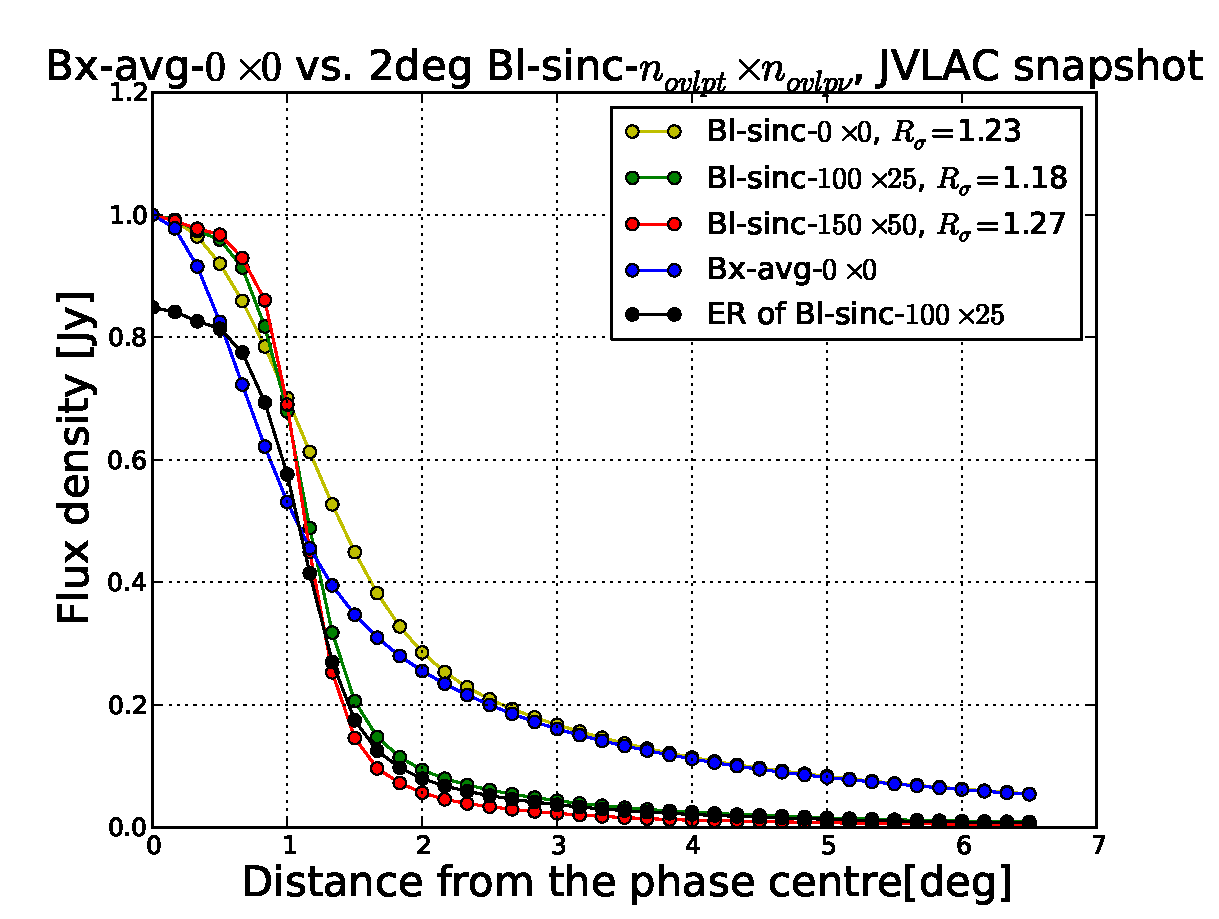
\includegraphics[width=1\textwidth]{./Figures/Bl-sinc-FoV2-vla.pdf}\caption{Time and frequency 
  direction sinc filter applied on a $2^{\circ}$ FoV JVLA surveys observing a 1Jy source move from the phase centre for 150s integration 
  synthesis at 6.25MHz bandwidth, natural weighting.}\label{fig:Bl-sinc-FoV2}\end{minipage}
  \hspace{1cm}
  \begin{minipage}{0.38\linewidth}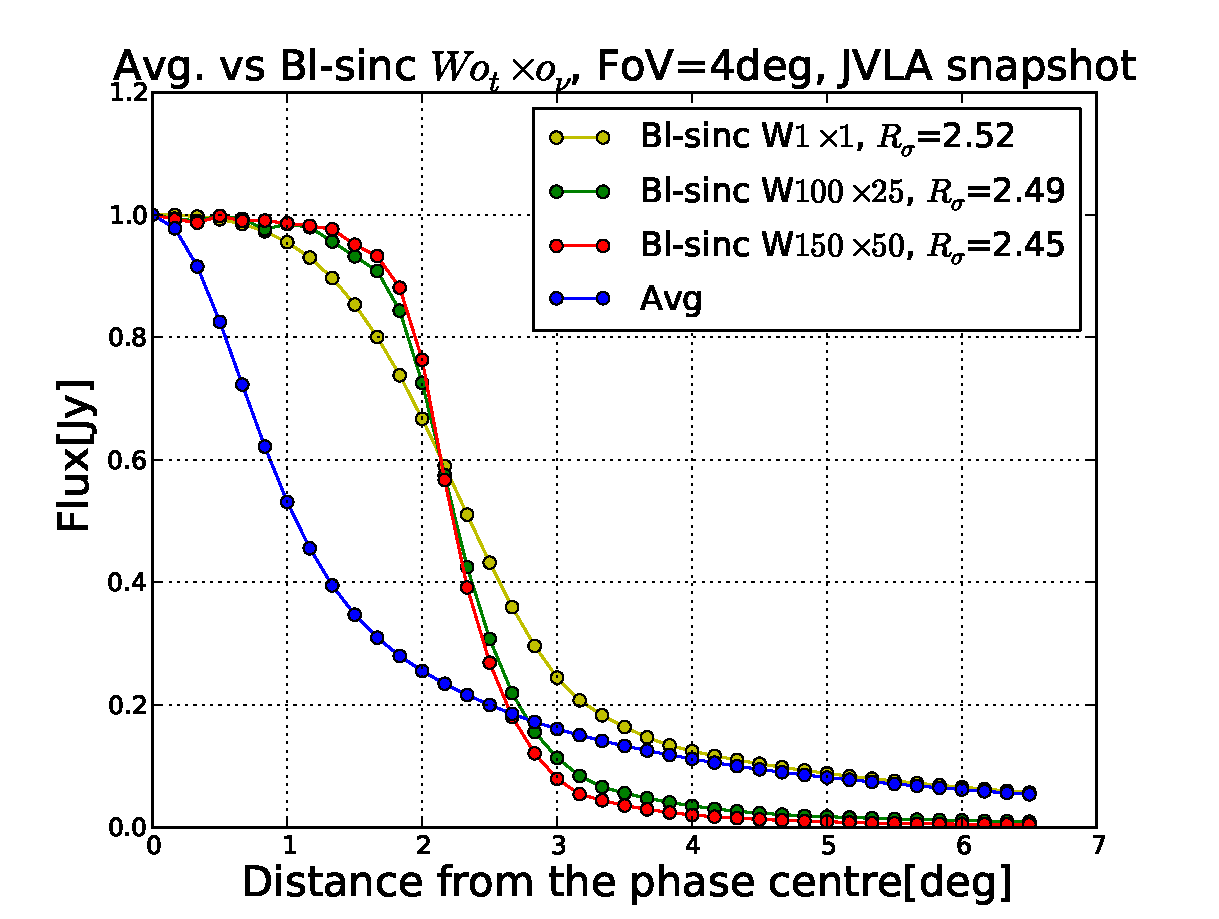
\includegraphics[width=1\textwidth]{./Figures/Bl-sinc-FoV4-vla.pdf}\caption{Time and frequency 
  direction sinc filter applied on a $4^{\circ}$ FoV JVLA surveys observing a 1Jy source move from the phase centre for 150s integration 
  synthesis at 6.25MHz bandwidth, natural weighting.}\label{fig:Bl-sinc-FoV4} 
  \end{minipage}\\
  \begin{minipage}{0.38\linewidth}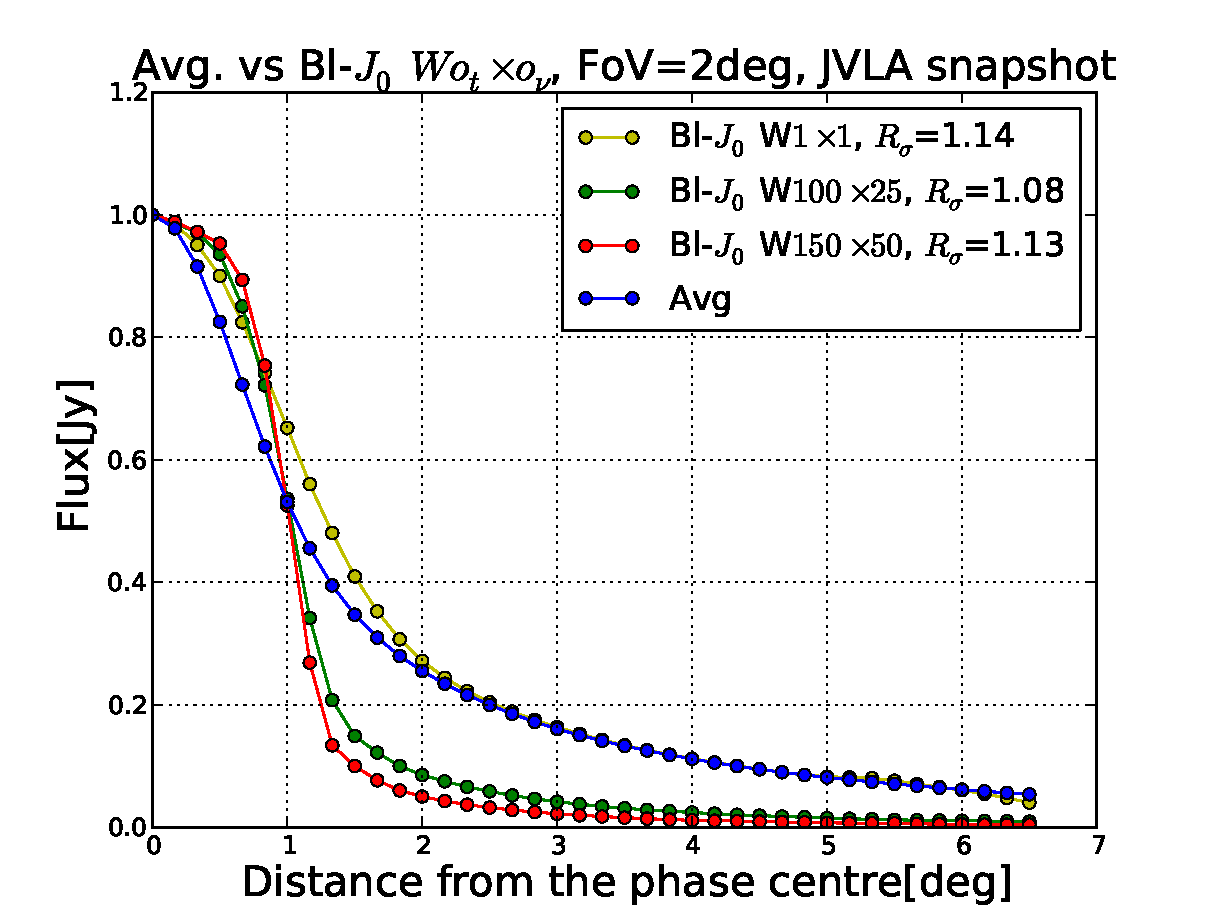
\includegraphics[width=1\textwidth]{./Figures/Bl-bessel-FoV2-vla.pdf}\caption{Time and frequency 
  direction Bessel first kind filter applied on a $2^{\circ}$ FoV JVLA surveys observing a 1Jy source move from the phase centre for 150s 
  integration synthesis at 6.25MHz bandwidth, natural weighting.}\label{fig:Bl-bessel-FoV2}\end{minipage}
  \hspace{1cm}
  \begin{minipage}{0.38\linewidth}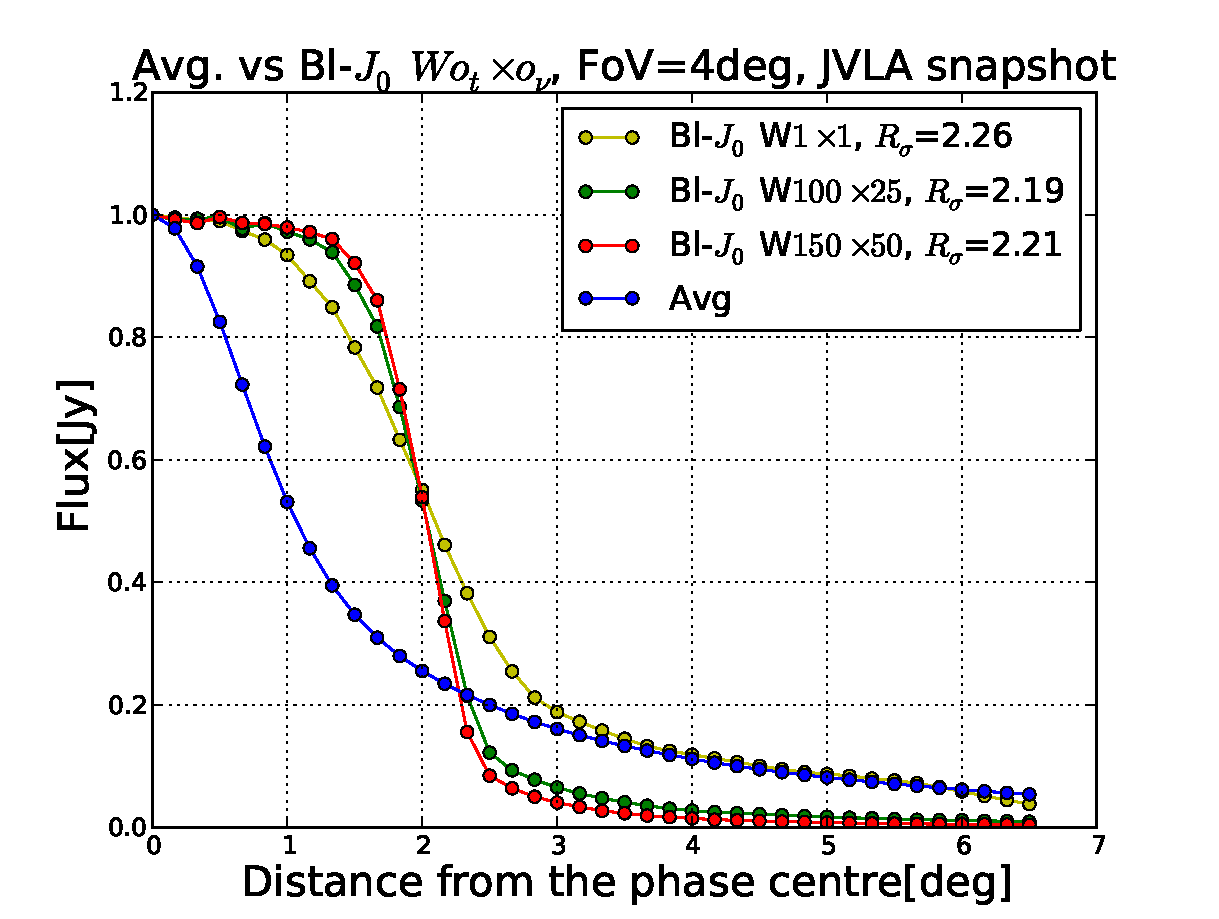
\includegraphics[width=1\textwidth]{./Figures/Bl-bessel-FoV4-vla.pdf}\caption{Time and frequency 
  direction Bessel first kind filter applied on a $4^{\circ}$ FoV JVLA surveys observing a 1Jy source move from the phase centre for 150s 
  integration synthesis at 6.25MHz bandwidth, natural weighting.}\label{fig:Bl-bessel-FoV4}\end{minipage}\\
  \begin{minipage}{0.38\linewidth}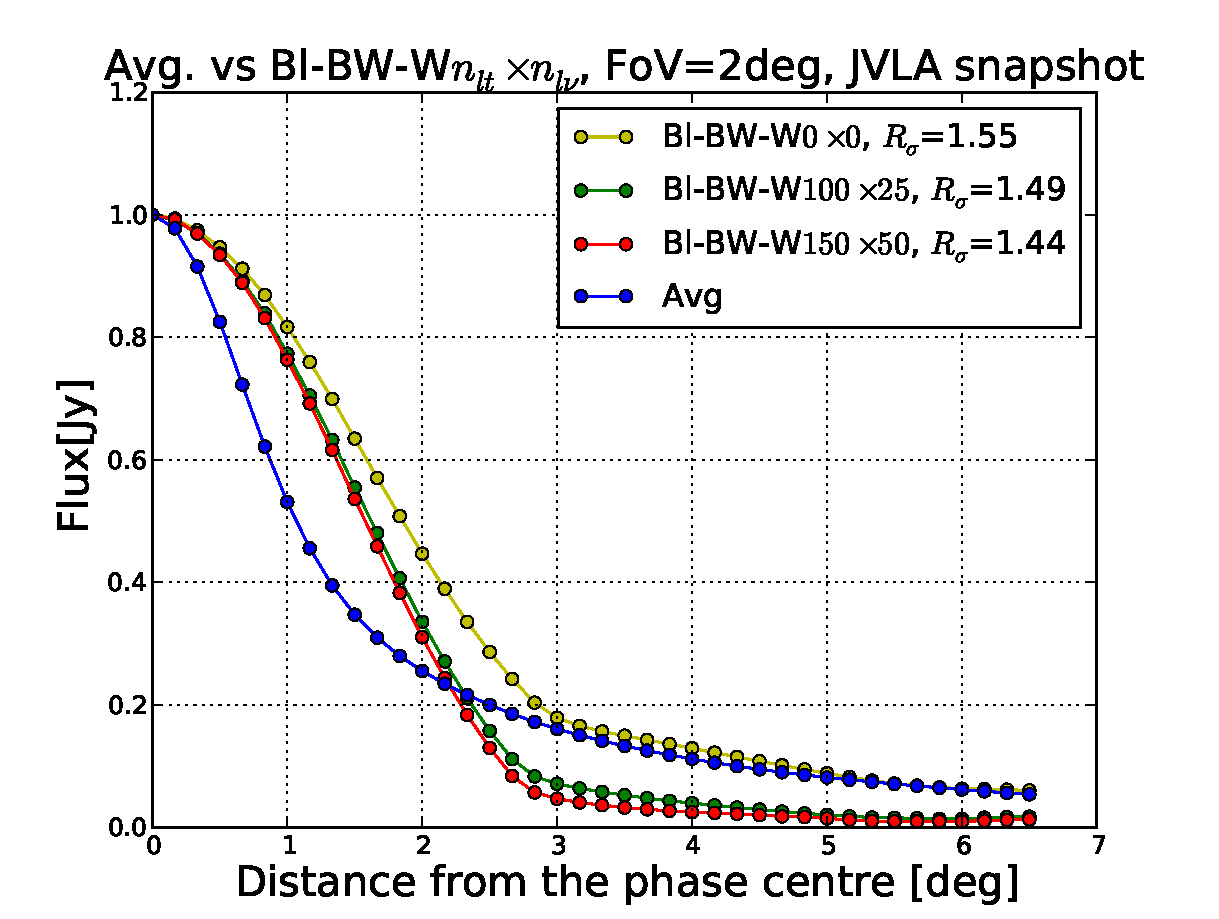
\includegraphics[width=1\textwidth]{./Figures/Bl-butter-FoV2-vla.pdf}\caption{Time and frequency 
  direction Butterwordth filter applied on a $2^{\circ}$ FoV JVLA surveys observing a 1Jy source move from the phase centre for 
  150s integration synthesis at 6.25MHz bandwidth, natural weighting.}\label{fig:Bl-butter-FoV2}\end{minipage}
  \hspace{1cm}
  \begin{minipage}{0.38\linewidth}
  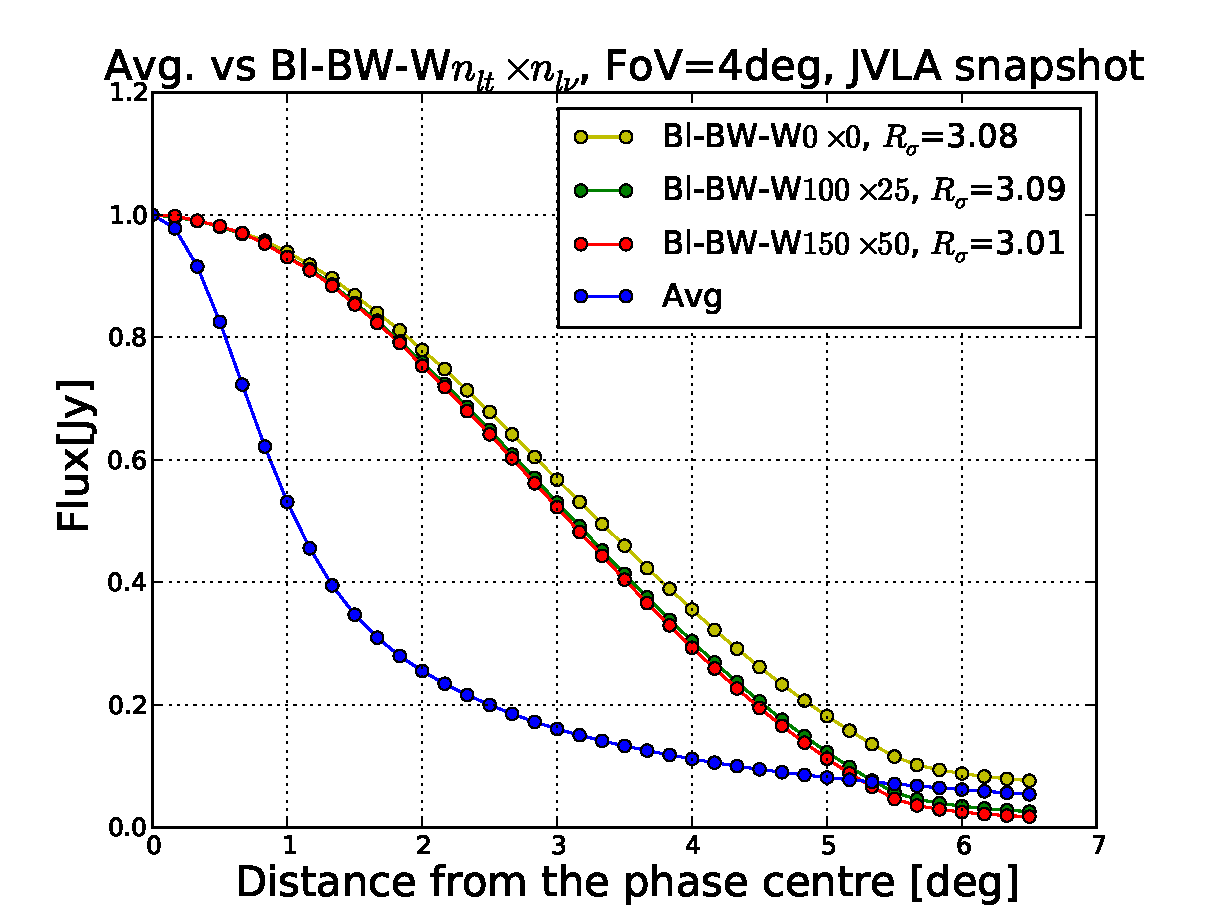
\includegraphics[width=1\textwidth]{./Figures/Bl-butter-FoV4-vla.pdf}
   \caption{Time and frequency 
   direction Butterwordth filter applied on a $4^{\circ}$ FoV JVLA surveys observing a 1Jy source move from the phase centre for 150s 
  integration synthesis at 6.25MHz bandwidth, natural weighting.}
  \label{fig:Bl-butter-FoV4}\end{minipage}
  \caption{Time and frequency 
  direction Butterwordth filter applied on a $4^{\circ}$ FoV JVLA surveys observing a 1Jy source move from the phase centre for 150s 
  integration synthesis at 6.25MHz bandwidth, natural weighting.}
  \end{figure*} 
  \begin{figure*}
    \centering
  \begin{minipage}{0.38\linewidth}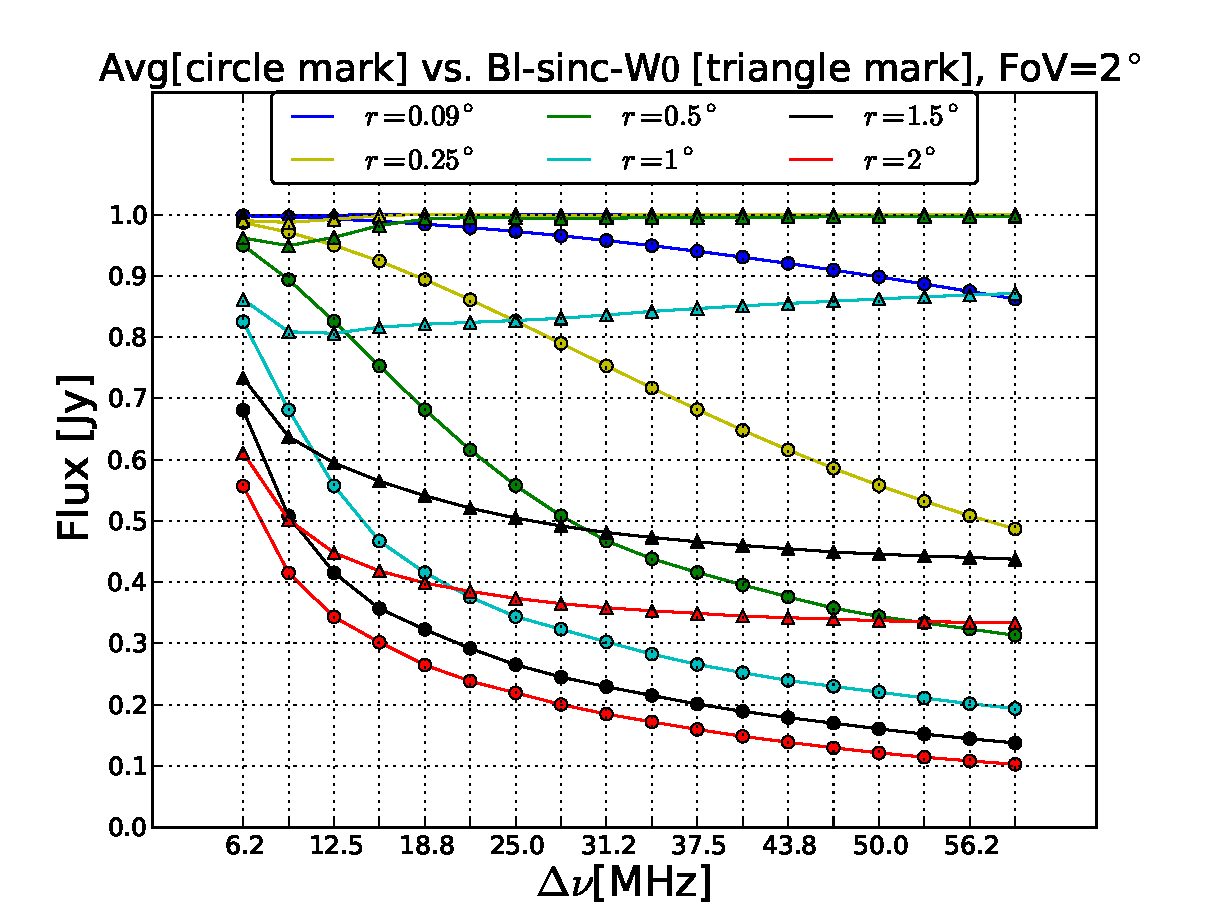
\includegraphics[width=1\textwidth]{./Figures/max-integ-freq-sinc-w1x1-fov2.pdf}
    \caption{Response to a 1Jy source at different positions, as a function of  bandwidth with $2^{\circ}$ frequency sinc filter.}
    \label{fig:max-integ-freq-sinc-w1x1-fov2}
  \end{minipage}
  \hspace{1cm}
  \begin{minipage}{0.38\linewidth}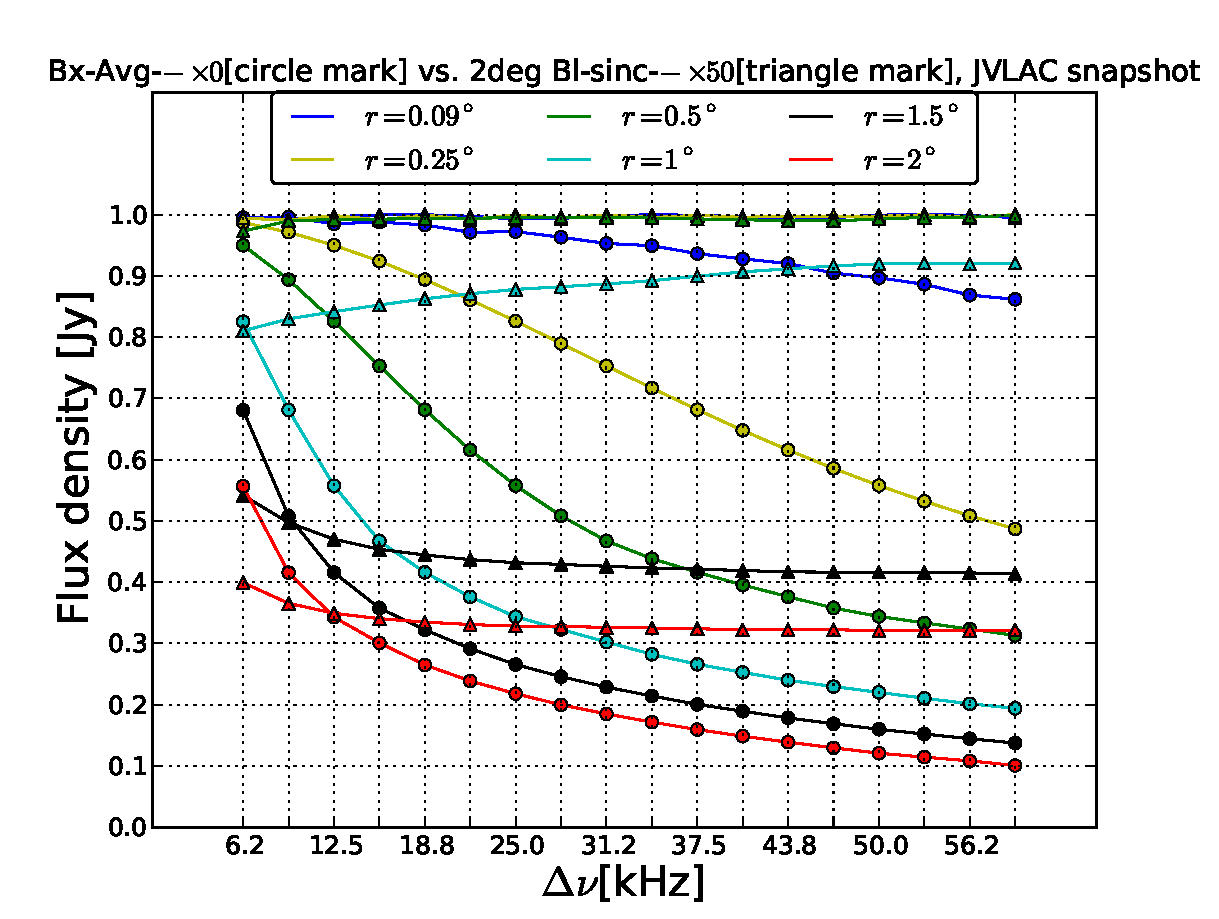
\includegraphics[width=1\textwidth]{./Figures/max-integ-freq-sinc-w1x50-fov2.pdf}
        \caption{Response to a 1Jy source at different positions, as a function of bandwidth with $2^{\circ}$ frequency overlap sinc 
filter.}
        \label{fig:max-integ-freq-sinc-w1x50-fov2}
        \end{minipage}\\
  \begin{minipage}{0.38\linewidth}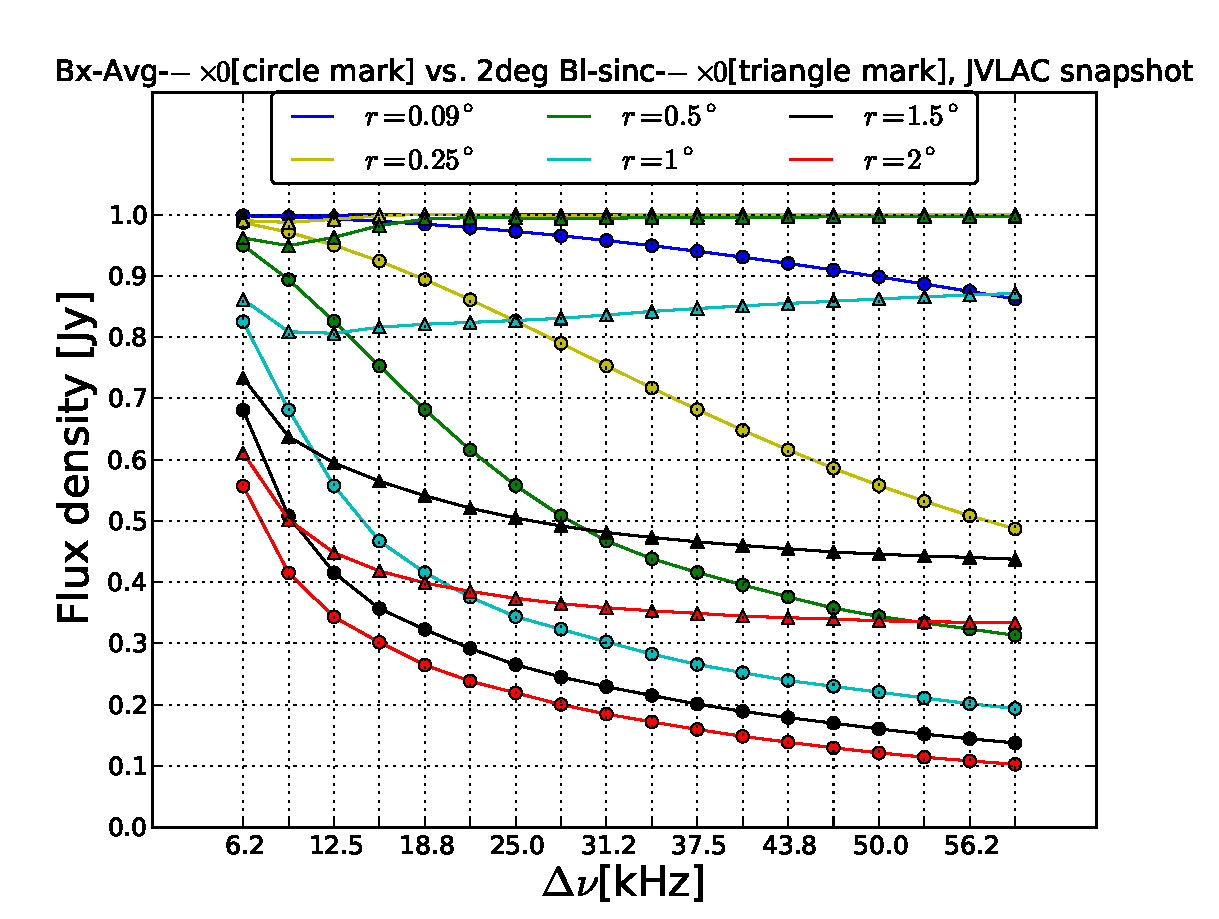
\includegraphics[width=1\textwidth]{./Figures/max-integ-freq-bessel-w1x1-fov2.pdf}
        \caption{Response to a 1Jy source at different positions, as a function of bandwidth with $2^{\circ}$ frequency Bessel first kind 
of 
  order zero filter.}
        \label{fig:max-integ-freq-bessel-w1x1-fov2}
        \end{minipage}
  \hspace{1cm}
  \begin{minipage}{0.38\linewidth}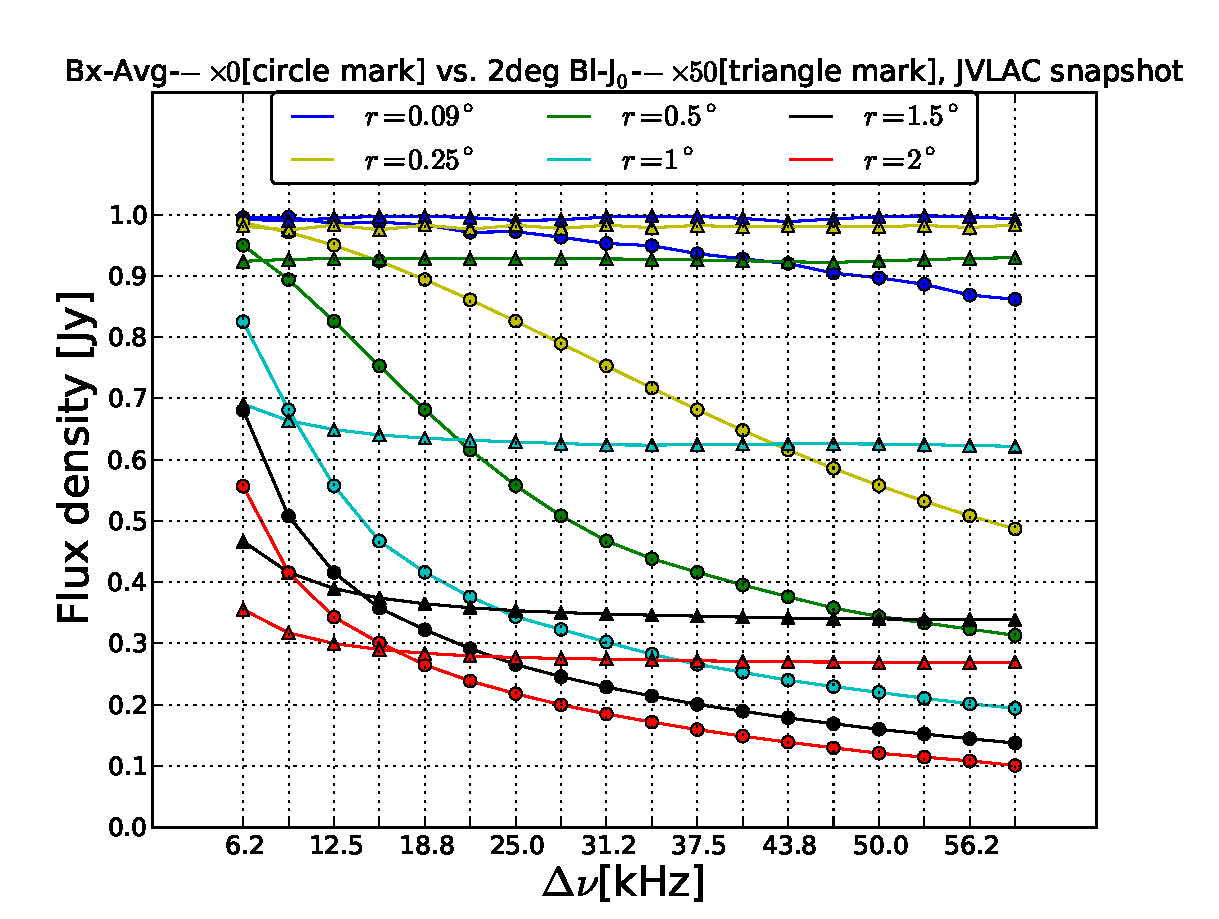
\includegraphics[width=1\textwidth]{./Figures/max-integ-freq-bessel-w1x50-fov2.pdf}
        \caption{Response to a 1Jy source at different positions, as a function of bandwidth with $2^{\circ}$ frequency overlap Bessel 
first kind filter of order zero filter.}
        \label{fig:max-integ-freq-bessel-w1x50-fov2}
        \end{minipage}
\begin{minipage}{0.38\linewidth}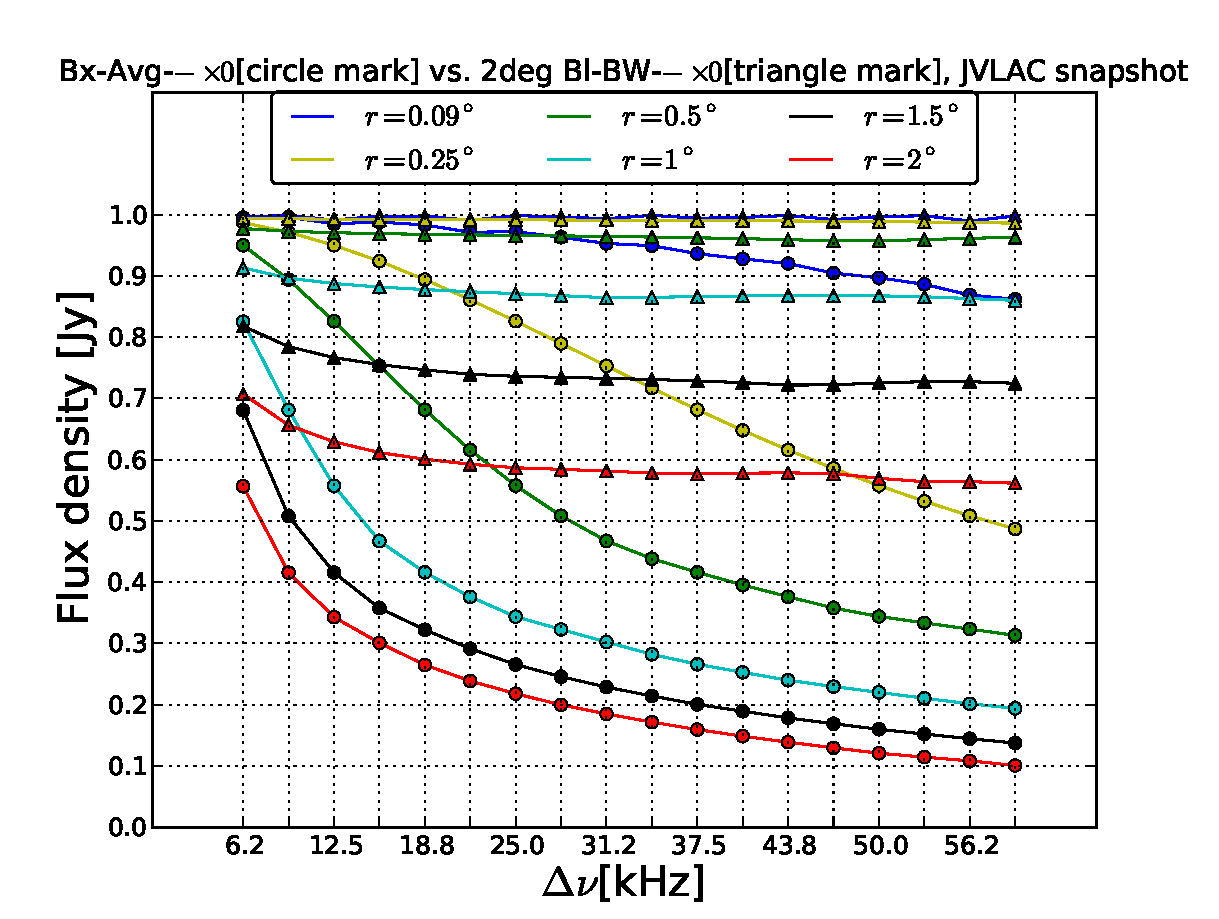
\includegraphics[width=1\textwidth]{./Figures/max-integ-freq-butter-w1x1-fov2.pdf}
      \caption{Response to a 1Jy source at different positions, as a function of bandwidth with $2^{\circ}$ frequency Butterwordth filter.}
      \label{fig:max-integ-freq-butter-w1x1-fov2}
      \end{minipage}
\hspace{1cm}
\begin{minipage}{0.38\linewidth}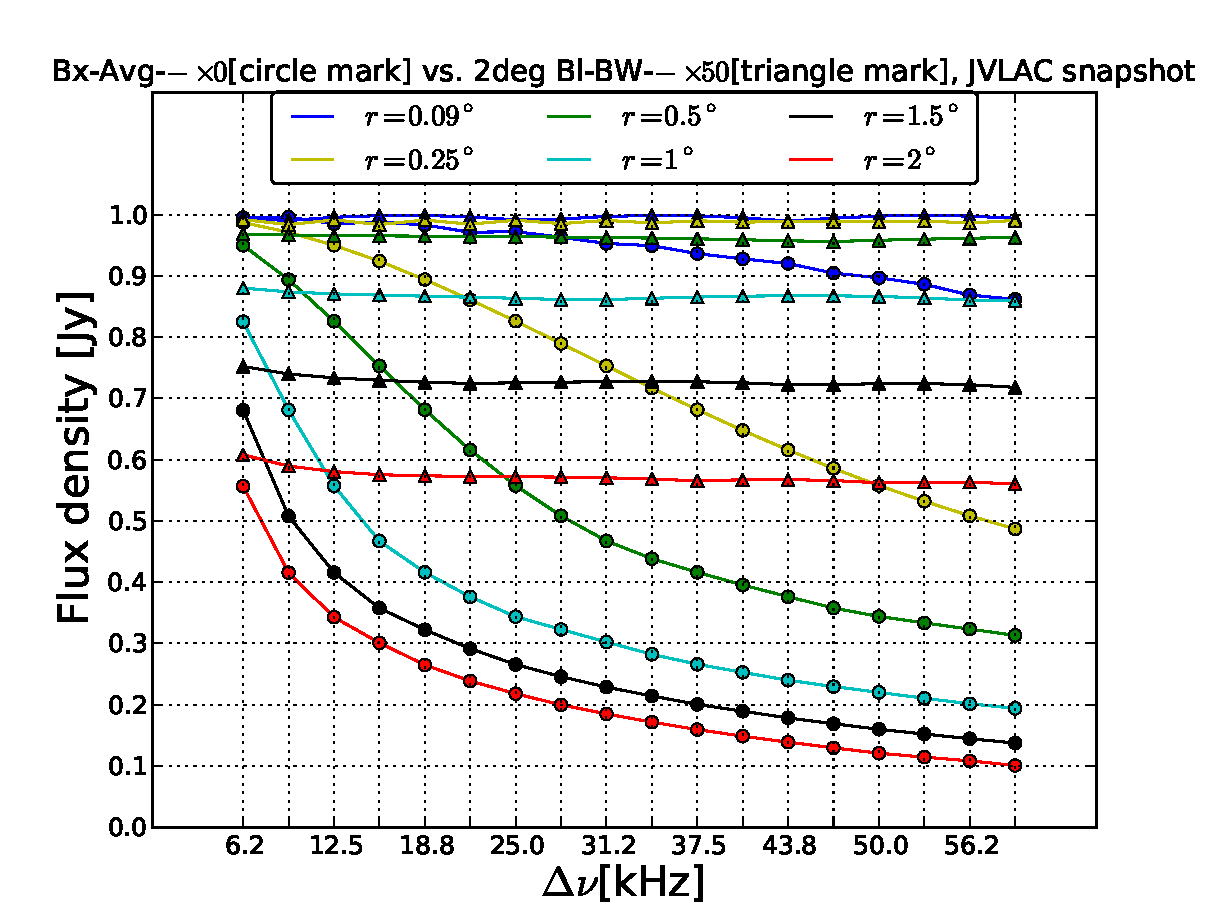
\includegraphics[width=1\textwidth]{./Figures/max-integ-freq-butter-w1x50-fov2.pdf}
      \caption{Response to a 1Jy source at different positions, as a function of bandwidth with $2^{\circ}$ frequency overlap Butterwordth 
filter.}
      \label{fig:max-integ-freq-butter-w1x50-fov2}
      \end{minipage}
\end{figure*}
\begin{figure*}
% *********************** Scripts that created these plots ***********************************
%plot.plot(wind1='/home/atemkeng/TempleFull/DATA/Maxtime-bessel-fov2-window/',title1=r'Avg[circle mark] vs. Bl-J$_0$-W$1\times 1$ [triangle 
	    %mark], FoV=2$^\circ$',xlabel=r'$\Delta t$[s]')
  \centering
\begin{minipage}{0.38\linewidth}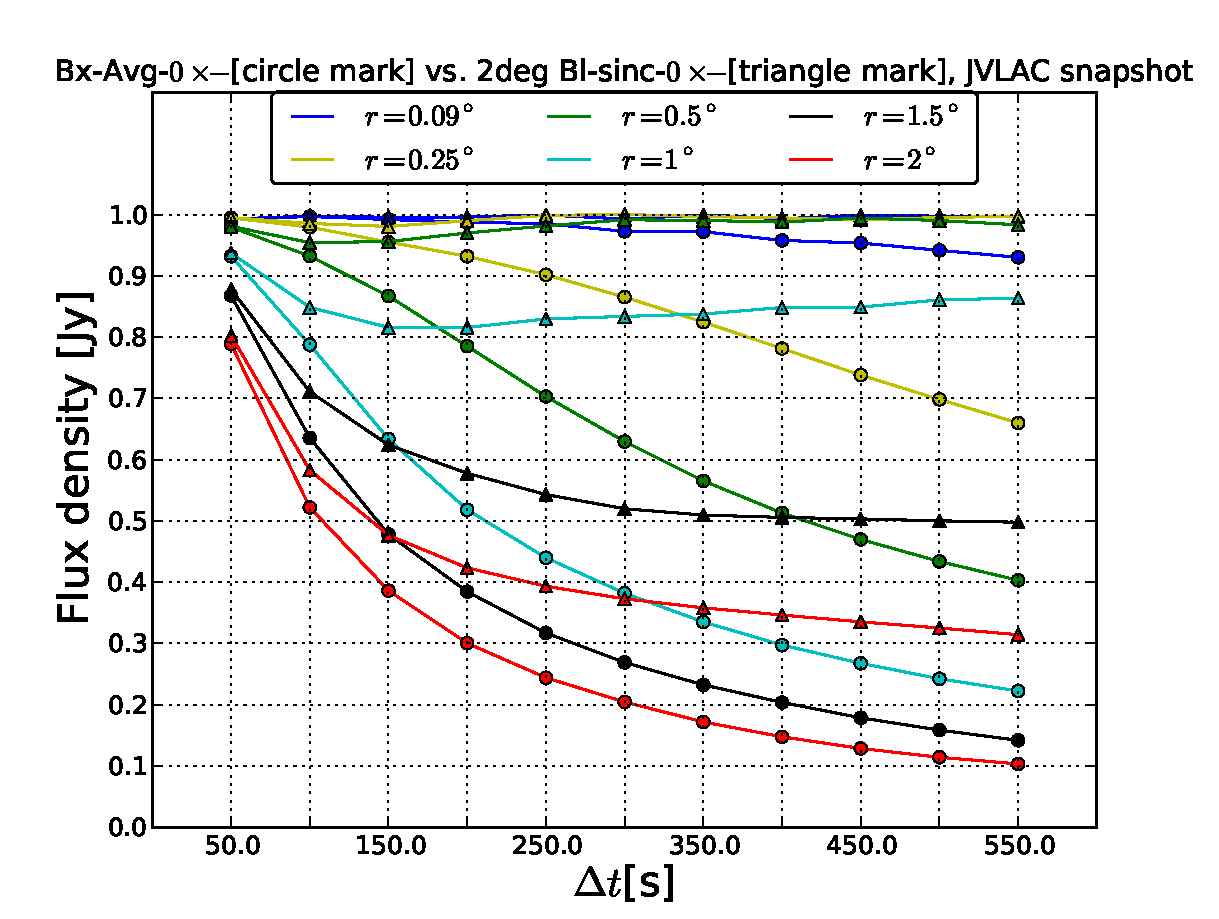
\includegraphics[width=1.\textwidth]{./Figures/max-integ-time-sinc-w1x1-fov2.pdf}
	\caption{Response to a 1Jy source at different positions, as a function of integration time with $2^{\circ}$ time sinc filter.}
	\label{fig:max-integ-time-sinc-w1x1-fov2}
	\end{minipage} \hspace{1cm}
\begin{minipage}{0.38\linewidth}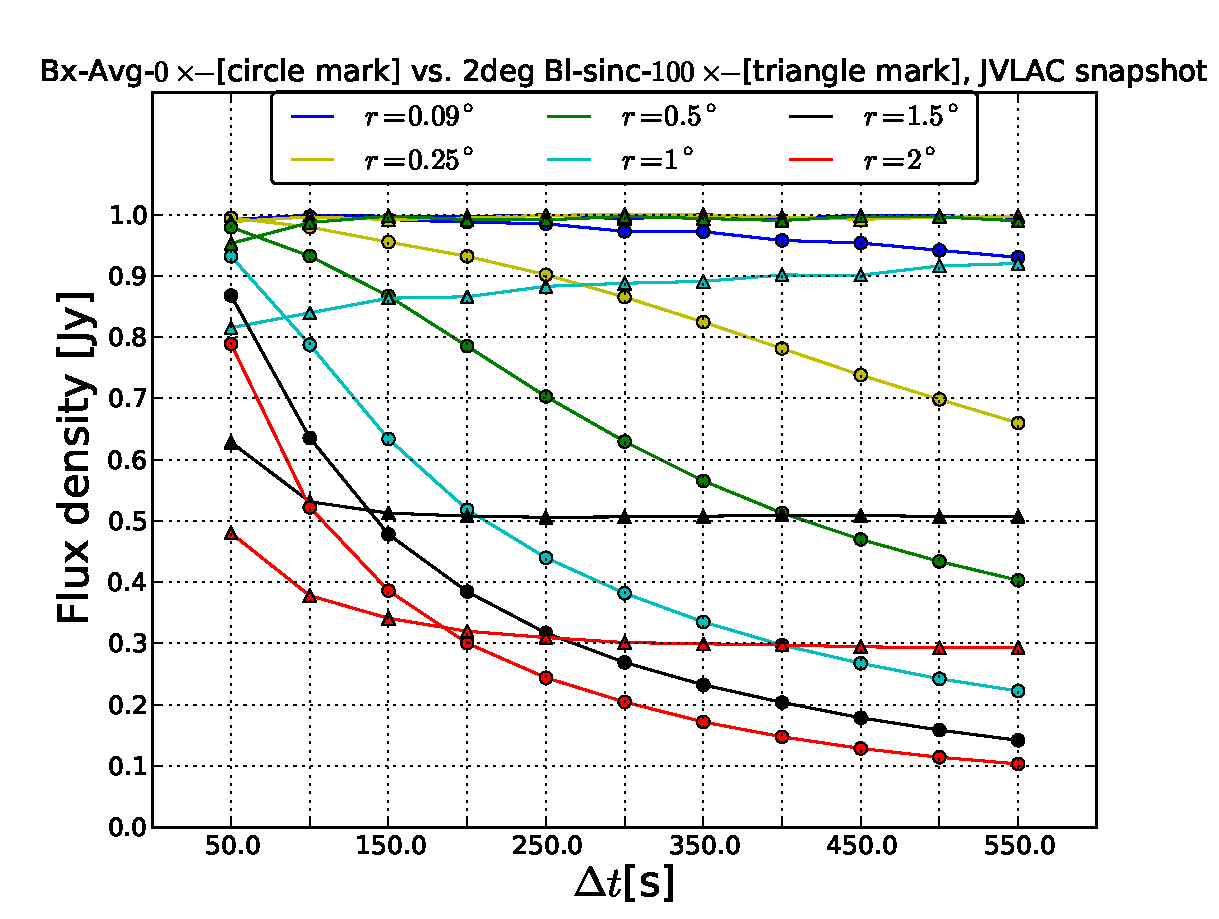
\includegraphics[width=1.\textwidth]{./Figures/max-integ-time-sinc-w100x1-fov2.pdf}
        \caption{Response to a 1Jy source at different positions, as a function of integration time with $2^{\circ}$ time overlap sinc 
filter.}
      \label{fig:max-integ-time-sinc-w100x1-fov2}
      \end{minipage}\\
\begin{minipage}{0.38\linewidth}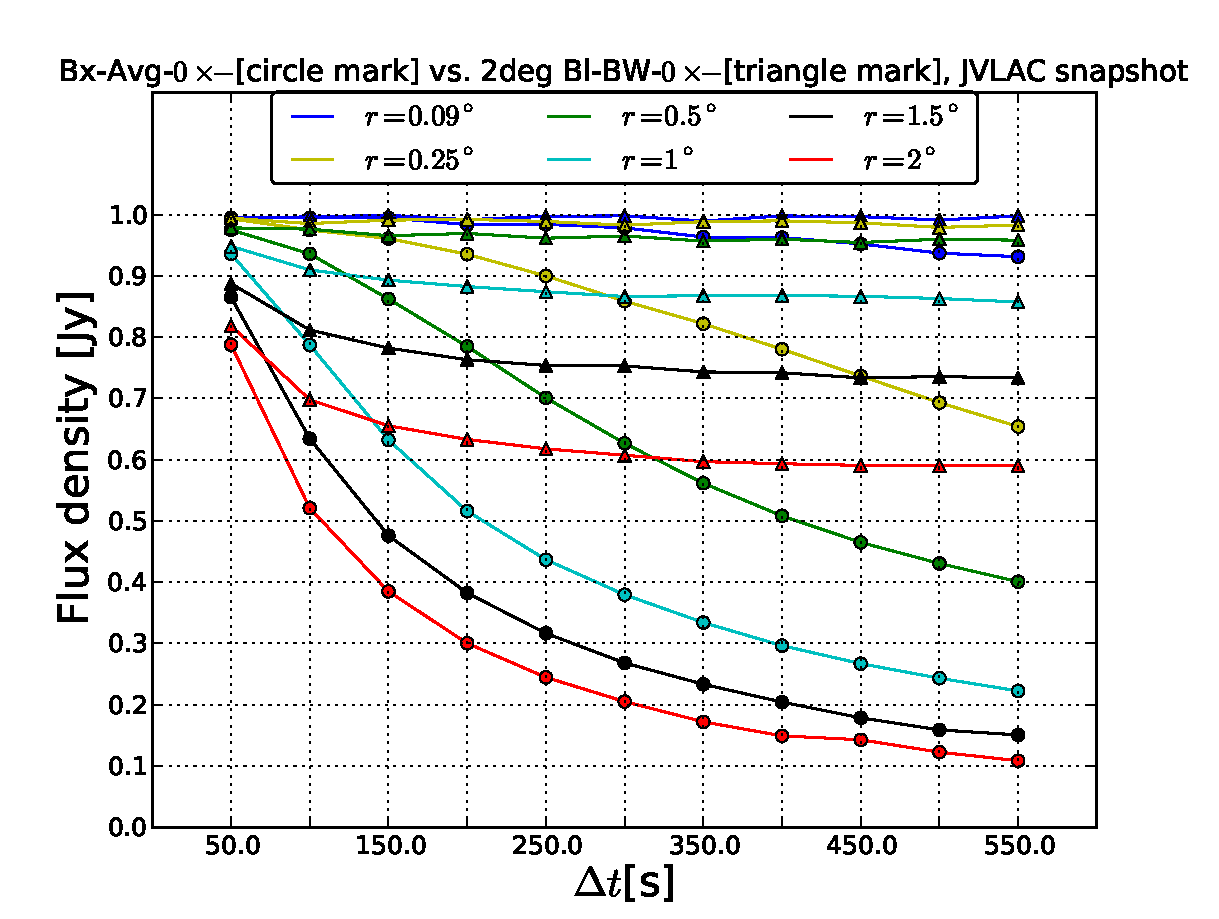
\includegraphics[width=1\textwidth]{./Figures/max-integ-time-bessel-w1x1-fov2.pdf}
    \caption{Response to a 1Jy source at different positions, as a function of integration time with $2^{\circ}$ time Bessel first kind of 
order zero
filter.}
    \label{fig:max-integ-time-bessel-w1x1-fov2}
    \end{minipage} 
 \hspace{1cm}
\begin{minipage}{0.38\linewidth}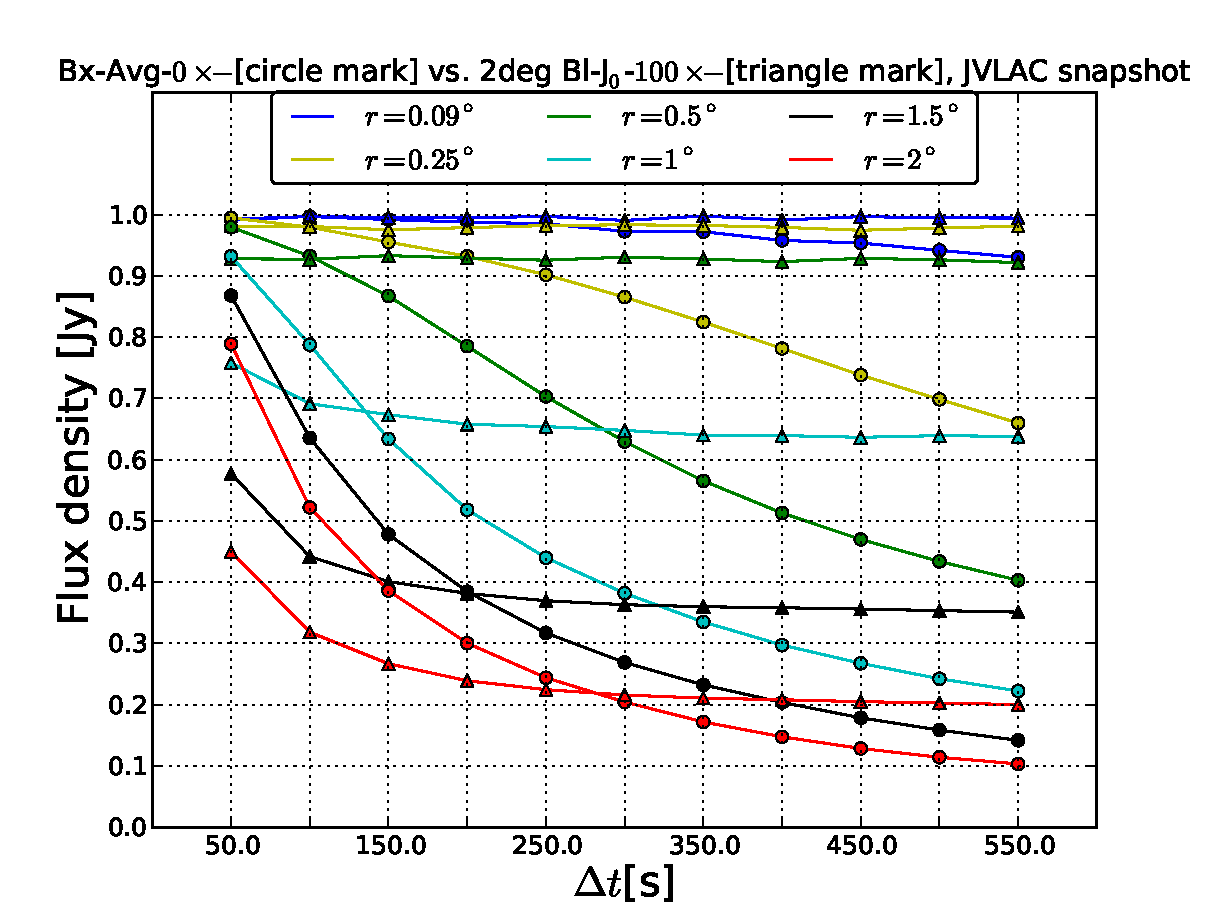
\includegraphics[width=1\textwidth]{./Figures/max-integ-time-bessel-w100x1-fov2.pdf}
    \caption{Response to a 1Jy source at different positions, as a function of integration time with $2^{\circ}$ time overlap 
      Bessel first kind of order zero filter.}
    \label{fig:max-integ-time-bessel-w100x1-fov2}\end{minipage}\\
\begin{minipage}{0.38\linewidth}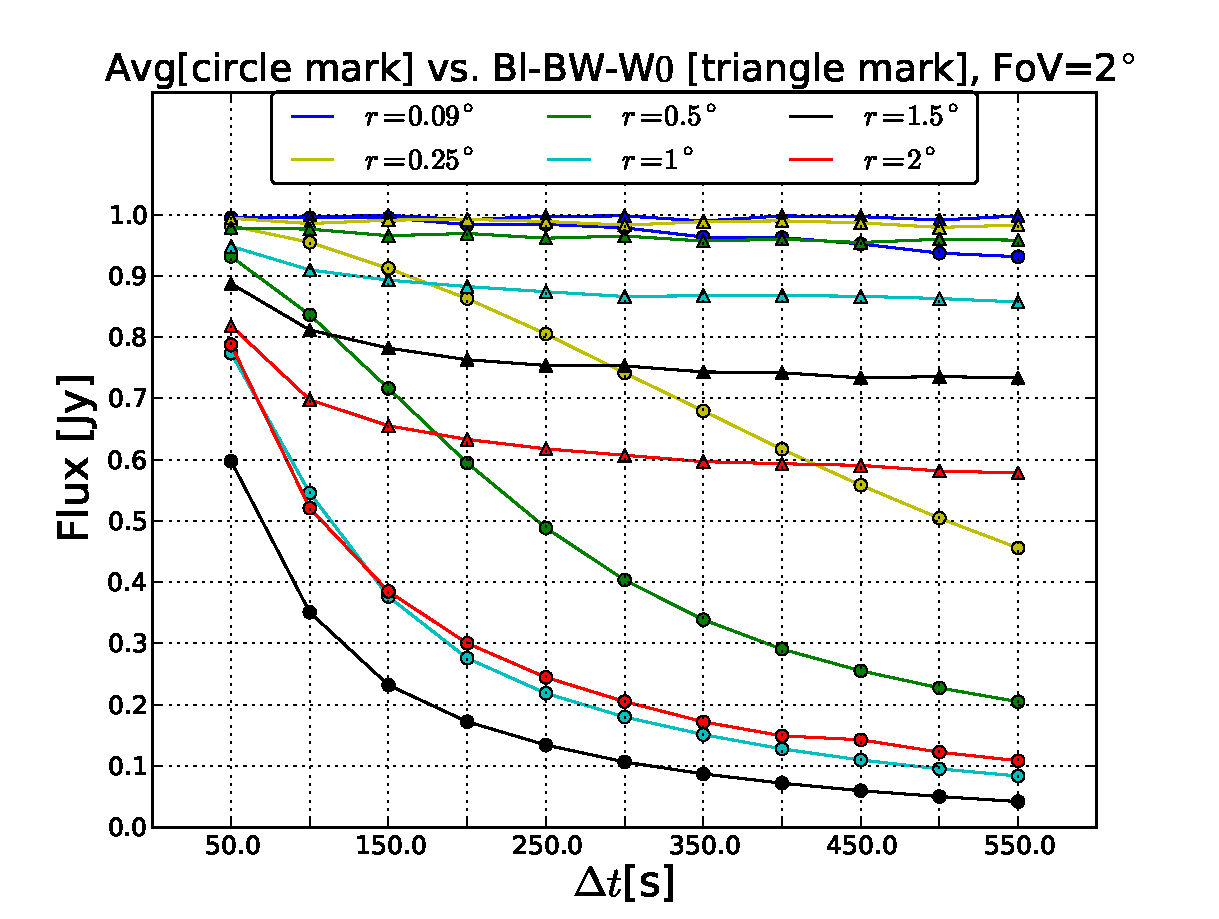
\includegraphics[width=1\textwidth]{./Figures/max-integ-time-butter-w1x1-fov2.pdf}
    \caption{Response to a 1Jy source at different positions, as a function of integration time with $2^{\circ}$ time Butterwordth 
filter.}
    \label{fig:max-integ-time-butter-w1x1-fov2}
    \end{minipage} 
 \hspace{1cm}
\begin{minipage}{0.38\linewidth}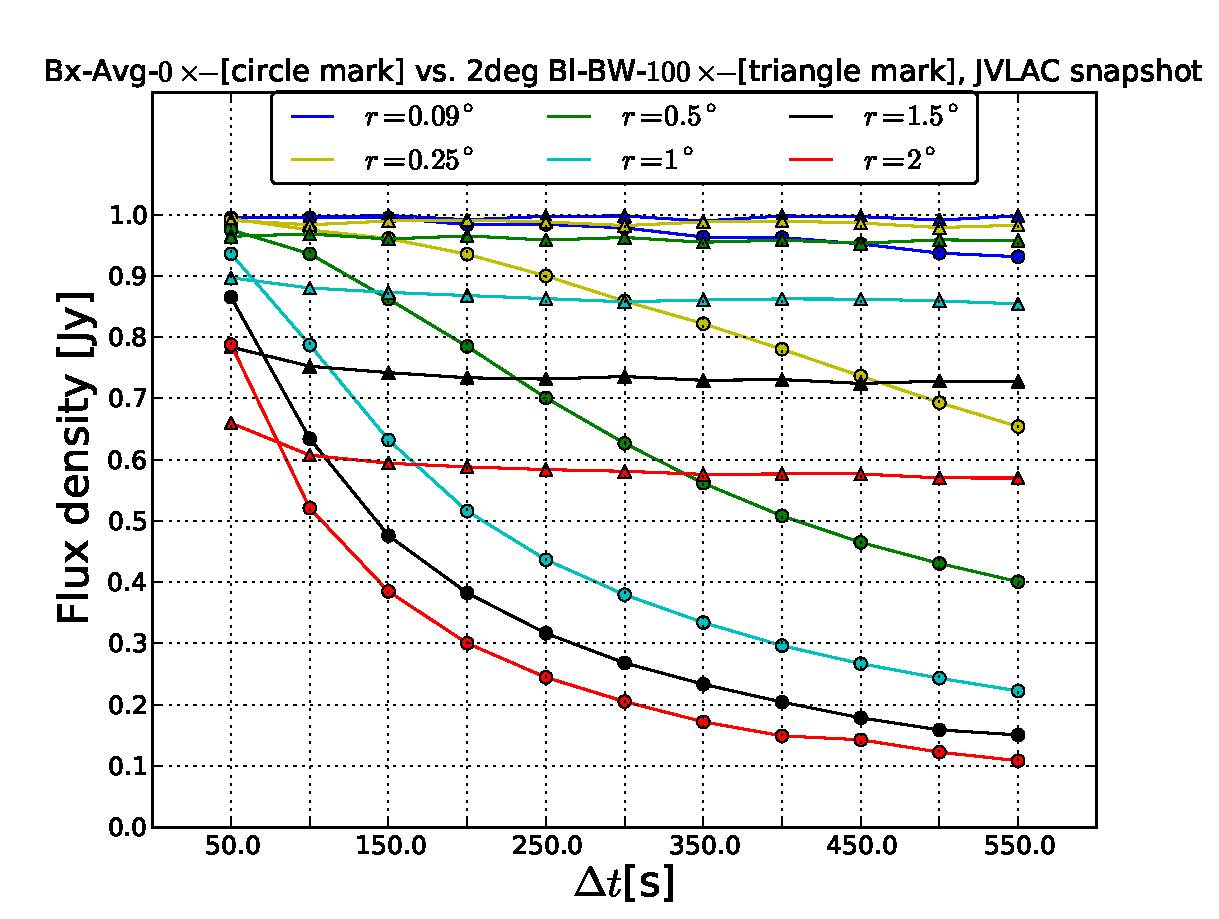
\includegraphics[width=1\textwidth]{./Figures/max-integ-time-butter-w100x1-fov2.pdf}
    \caption{Response to a 1Jy source at different positions, as a function of integration time with $2^{\circ}$ time overlap 
      Butterwordth filter.}
    \label{fig:max-integ-time-butter-w100x1-fov2}\end{minipage}   
\end{figure*}
\begin{figure*}
  \centering
\begin{minipage}{0.38\linewidth}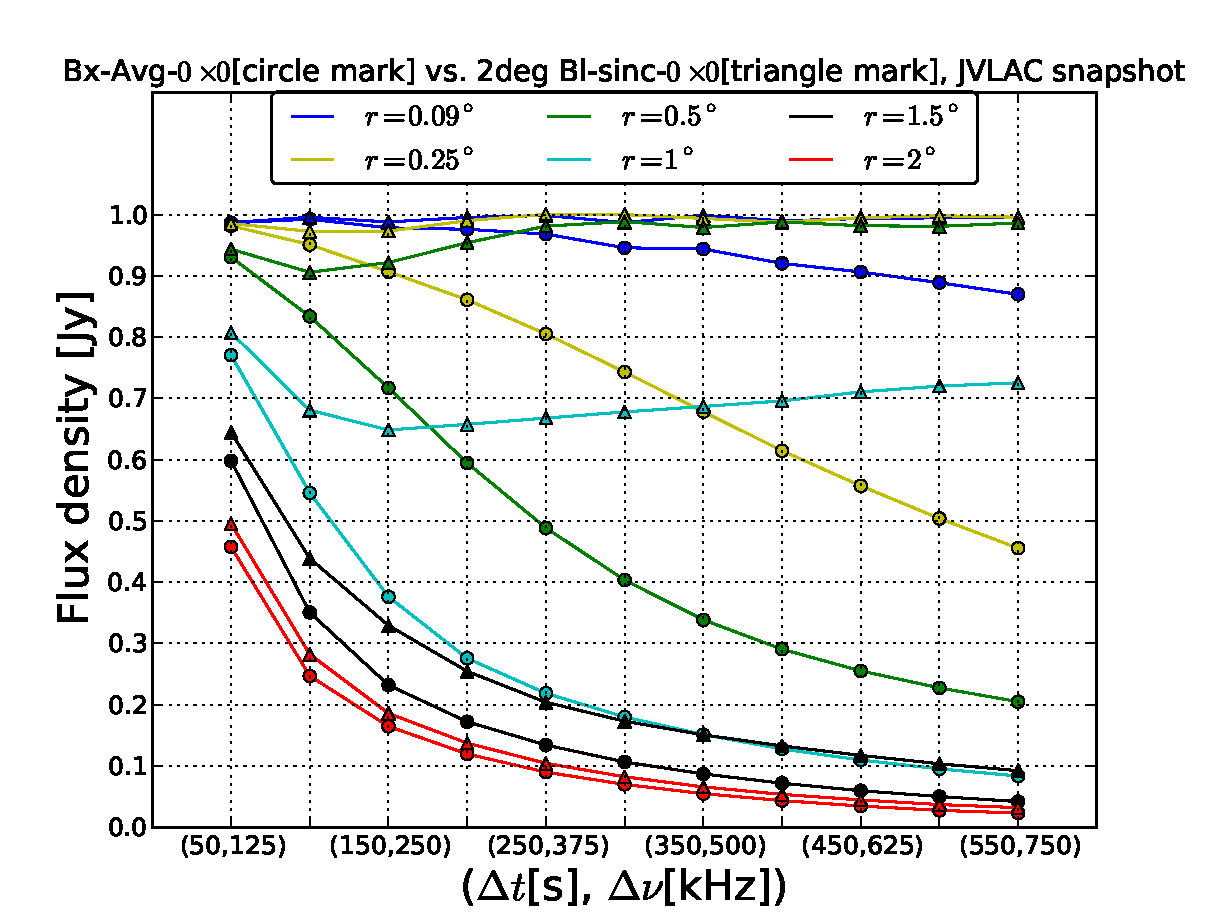
\includegraphics[width=1\textwidth]{./Figures/max-integ-timefreq-sinc-w1x1-fov2.pdf}
    \caption{Response to a 1Jy source at different positions, as a function of integration time and bandwidth; with $2^{\circ}$ frequency 
sinc filter.}
    \label{fig:max-integ-timefreq-sinc-w1x1-fov2}\end{minipage}
 \hspace{1cm}
\begin{minipage}{0.38\linewidth}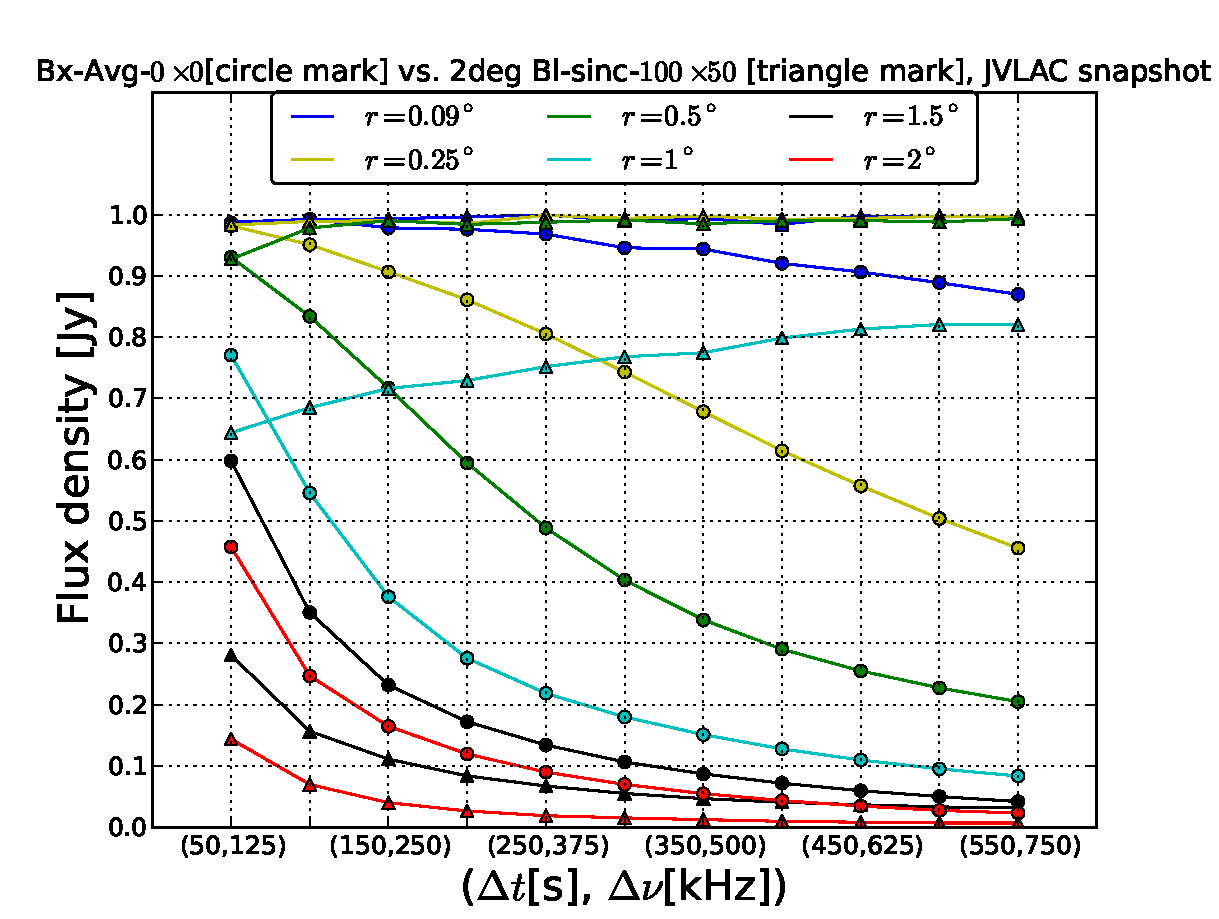
\includegraphics[width=1\textwidth]{./Figures/max-integ-timefreq-sinc-w100x50-fov2.pdf}
    \caption{Response to a 1Jy source at different positions, as a function of integration time and bandwidth; with $2^{\circ}$ frequency 
 overlap sinc filter.}
    \label{fig:max-integ-timefreq-sinc-w100x50-fov2}\end{minipage}\\
\begin{minipage}{0.38\linewidth}\includegraphics[width=1\textwidth]{./Figures/max-integ-timefreq-bessel-w1x1-fov2.pdf}
      \caption{Response to a 1Jy source at different positions, as a function of integration time and bandwidth, with $2^{\circ}$ frequency 
Bessel first kind of order zero filter.}
      \label{fig:max-integ-timefreq-bessel-w1x1-fov2}\end{minipage}
\hspace{1cm}
\begin{minipage}{0.38\linewidth}\includegraphics[width=1\textwidth]{./Figures/max-integ-timefreq-bessel-w100x50-fov2.pdf}
      \caption{Response to a 1Jy source at different positions, as a function of integration time and bandwidth, with $2^{\circ}$ frequency 
overlap Bessel first kind of order zero filter.}
  \label{fig:max-integ-timefreq-bessel-w100x50-fov2}\end{minipage}
\begin{minipage}{0.38\linewidth}\includegraphics[width=1\textwidth]{./Figures/max-integ-timefreq-butter-w1x1-fov2.pdf}
      \caption{Response to a 1Jy source at different positions, as a function of integration time and bandwidth, with $2^{\circ}$ frequency 
Butterwordth filter.}
      \label{fig:max-integ-timefreq-butter-w1x1-fov2}\end{minipage}
\hspace{1cm}
\begin{minipage}{0.38\linewidth}\includegraphics[width=1\textwidth]{./Figures/max-integ-timefreq-butter-w100x50-fov2.pdf}
      \caption{Response to a 1Jy source at different positions, as a function of integration time and bandwidth, with $2^{\circ}$ frequency 
overlap Butterwordth filter.}
  \label{fig:max-integ-timefreq-butter-w100x50-fov2}\end{minipage}
\end{figure*}
\section{Conclusions}
The goal of this paper was threefold. The original motivation behind the work presented in this

paper was to **** windowing functions***\\
The second objective  was to study ****first algorithm data compression***\\
The final objective was to ****second algorithm data compression and out field suppression*** \\
Drawback and futures works*** drawback and futures works*****
\section*{Acknowledgements}
The research  made use of  MeqTrees software system designed to implement numerical models for third-generation calibration (3GC) 
 Python Extensions for Interferometry and Python. The research has been supported by the South Africa National Research Foundation.
\bibliographystyle{mn2e}
\bibliography{m_paper}
\appendix
\section[]{Derivation of complex matrices}
\label{app:complexmatrices}
The complex matrices used in section \ref{sec:imaging} are explicitly derived in this appendix. In Eq.\ref{eqbb:linear}, the matrices
$\mathbf{C}_{(t,\nu)}^{block}$ and $\mathbf{W}_{pq,(t,\nu)}^{block}$ are blocks diagonals  both of size $(4n_t n_{\nu})\times(4n_t 
n_{\nu})$ explicitly expressed as follow:
\begin{equation*}
\mathbf{C}_{(t,\nu)}^{block}=
  \begin{bmatrix}
    \mathbf{c}_{(t,\nu)} & 0 & 0 & 0\\
    0 &  \mathbf{c}_{(t,\nu)} &0 & 0 \\
    0 & 0 & \mathbf{c}_{(t,\nu)} & 0\\
      0 & 0 & 0 & \mathbf{c}_{(t,\nu)}\\
  \end{bmatrix}
\end{equation*}
\begin{equation*}
\mathbf{W}_{pq,(t,\nu)}^{block}=
  \begin{bmatrix}
    \mathbf{W}_{pq,(t,\nu)}& 0 & 0 & 0\\
    0 &  \mathbf{W}_{pq,(t,\nu)} &0 & 0 \\
    0 & 0 & \mathbf{W}_{pq,(t,\nu)} & 0\\
      0 & 0 & 0 & \mathbf{W}_{pq,(t,\nu)}\\
  \end{bmatrix}
\end{equation*}
In Eq.\ref{eq2:block}, the matrices $\mathbf{C}_{pq,(t,\nu)}^{block,n_{block}}$ and 
$\mathbf{W}_{pq,(t,\nu)}^{block,n_{block}}$ are blocks diagonals both of size $(4N_v^{pq}n_t n_{\nu})\times (4N_v^{pq}n_t n_{\nu})$, and 
the sampled visibilities $\mathbf{V}_{pq,(t,\nu)}^{samp,nblock}$ is a one row matrix of size $(N_v^{pq}4 n_t n_{\nu})\times (4 n_t 
n_{\nu})$ 
made of $\textbf{V}_{pq,(t,\nu)}^{samp}$. These matrices are explicitly expressed as follow:
\begin{equation*}
\mathbf{C}_{pq,(t,\nu)}^{block,n_{block}}=
  \begin{bmatrix}
    \mathbf{C}_{pq,(t,\nu)}^{block} &\dots & 0 & \dots & 0\\
    \vdots & \vdots & \vdots & \vdots & \vdots\\
    0 & \dots& \mathbf{C}_{pq,(t,\nu)}^{block} &\dots & 0\\
    \vdots & \vdots & \vdots & \vdots & \vdots \\
    0 & \dots& 0 &\dots & \mathbf{C}_{pq,(t,\nu)}^{block}\\
  \end{bmatrix}
\end{equation*}
\begin{equation*}
\mathbf{W}_{pq,(t,\nu)}^{block,n_{block}}=
  \begin{bmatrix}
    \mathbf{W}_{pq,(t,\nu)}^{block} &\dots & 0 & \dots & 0\\
    \vdots & \vdots & \vdots & \vdots & \vdots\\
    0 & \dots& \mathbf{W}_{pq,(t,\nu)}^{block} &\dots & 0\\
    \vdots & \vdots & \vdots & \vdots & \vdots \\
    0 & \dots& 0 &\dots & \mathbf{W}_{pq,(t,\nu)}^{block}\\
  \end{bmatrix}
\end{equation*}
\begin{eqnarray*}
\mathbf{V}_{pq,(t,\nu)}^{samp,n_{block}}&=&\Big(\mathbf{V}_{pq,(t,\nu)}^{samp,1},\dots, \mathbf{V}_{pq,(t,\nu)}^{samp,k}, \dots,
\mathbf{V}_{pq,(t,\nu)}^{samp,N^{pq}_v}\Big)^{\dagger}. 
\end{eqnarray*}
In Eq.\ref{eq:noise}, the matrix $\mathbf{B}$ of size $(N_v 4 n_t n_{\nu})\times (4 n_t n_{\nu})$ is defined as follow:
\begin{equation*}
\mathbf{B}_{}=
  \begin{bmatrix}
    \mathbf{C}_{01,(t,\nu)}^{block,n_{block}}\cdot \mathbf{W}_{01,(t,\nu)}^{block,n_{block}}\\
    \vdots\\
    \mathbf{C}_{ik,(t,\nu)}^{block,n_{block}}\cdot \mathbf{W}_{ik,(t,\nu)}^{block,n_{block}}\\
    \vdots \\
    \mathbf{C}_{jl,(t,\nu)}^{block,n_{block}}\cdot \mathbf{W}_{jl,(t,\nu)}^{block,n_{block}}
  \end{bmatrix}
\end{equation*}
% \section[]{Sky tapering function with averaging}
% \label{label:similarimaging}
% The measured sky intensity of the array is derived from the inverse Fourier transform of the sum of the sample visibilities 
% measured at each baseline.
% \begin{eqnarray*}
%  \mathcal{I}^{D}_{l,m}&=& \mathcal{F}^{-1}\Bigg\{\sum_{pq} c_{pq,(t,\nu)}\cdot\Big(\Pi_{pq}\circ V_{pq}^{samp}\Big)_{(t,\nu)}\Bigg\}\\
% 		      &=&\sum_{pq} \mathcal{F}^{-1}\{c_{pq,(t,\nu)}\}\circ \Big(\mathcal{F}^{-1}\{\Pi_{pq,(t,\nu)}\}\cdot 
% \mathcal{F}^{-1}\{V_{pq,(t,\nu)}^{samp}\}\Big)
% \end{eqnarray*}
% \begin{eqnarray*}	     
% \mathcal{I}^{D}_{l,m}&=&\sum_{pq}\mathcal{F}^{-1}\{\Pi_{pq,(t,\nu)}\}\cdot\bigg(\mathcal{F}^{-1}\{S_{pq}\cdot V_{pq,(t,\nu)}\}
% \bigg)
% \end{eqnarray*}
% recall from section \ref{sec:AvgCon} that $S_{pq}$ is the sampling function of the baseline $pq$ and $\Pi_{pq,(t,\nu)}$ is the 
% boxcar window.  This can be re-written as
% \begin{eqnarray*}	     
% \mathcal{I}^{D}_{l,m}&=&\sum_{pq} \mathcal{R}_{pq} \cdot\bigg(\mathcal{B}_{pq}\circ \mathcal{I}^{sky}_{l,m}\bigg)
% \end{eqnarray*}
% If all baselines are seen the same sky, then we can write:
% \begin{eqnarray*}	     
% \mathcal{I}^{D}_{l,m}&=&\mathcal{R}_{}\cdot\Bigg(\bigg(\sum_{pq}\mathcal{B}_{pq}\bigg)\circ \mathcal{I}^{sky}_{l,m}\Bigg)
% \end{eqnarray*}
% Here, $\mathcal{B}_{pq}$ is the point spread function for the baseline $pq$ and $\mathcal{R}_{pq}= \mathcal{R}$ is the sky taper, where 
% $\mathcal{R}_{}=sinc$.\\
% \\
\bsp
\label{lastpage}
\end{document}
